
% VLDB template version of 2020-08-03 enhances the ACM template, version 1.7.0:
% https://www.acm.org/publications/proceedings-template
% The ACM Latex guide provides further information about the ACM template

\documentclass[sigconf, nonacm]{acmart}

\usepackage{textcomp}
\usepackage{xcolor}
\usepackage{soul}

\usepackage{graphicx}
\usepackage{balance}  % for  \balance command ON LAST PAGE  (only there!)

\usepackage{color}
\usepackage{multirow}
\usepackage{subcaption}
% \usepackage{times}
\usepackage[export]{adjustbox}
%\usepackage{subfigure}
%\usepackage{times}
\usepackage[normalem]{ulem}
\useunder{\uline}{\ul}{}
% newly added
\usepackage{bbm}

\newcommand{\todo}[1]{[\textcolor{red}{TODO: #1}]}

\newcommand{\carrie}[1]{[\textcolor{blue}{Carrie: #1}]}

\newcommand{\LL}[1]{\textcolor{violet}{#1}}
\newcommand{\laks}[1]{\textcolor{teal}{\textbf{Laks: #1}}}
\newcommand{\stitle}[1]{\noindent\textup{\textbf{#1}}}

\newcommand{\rey}[1]{\textcolor{orange}{\textbf{Rey: #1}}}

%%%%%%%%%%%%%%%%%% macros 
\newcommand{\eat}[1]{}
\newcommand{\sprint}{\text{{\footnotesize SPRinT}}\xspace}
\newcommand{\sprintv}{\text{{\footnotesize SPRinT-V}}\xspace} 
\newcommand{\sprintc}{\text{{\footnotesize SPRinT-C}}\xspace} 
% \newcommand{\sprintpqa}{{$\text{SPRinT}_{\text{PQA}}$\xspace}}  
% \newcommand{\LL}[1]{\textcolor{purple}{#1}}
% \newcommand{\laks}[1]{\textcolor{cyan}{\textbf{[[Laks: #1]] }}}
\newcommand{\say}[1]{\textcolor{green}{Sihem: #1}}

\newcommand{\squishlist}{
 \begin{list}{$\bullet$}
  { \setlength{\itemsep}{0pt}
     \setlength{\parsep}{3pt}
     \setlength{\topsep}{3pt}
     \setlength{\partopsep}{0pt}
     \setlength{\leftmargin}{1.5em}
     \setlength{\labelwidth}{1em}
     \setlength{\labelsep}{0.5em} } }

\newcommand{\squishlisttwo}{
 \begin{list}{$\bullet$}
  { \setlength{\itemsep}{0pt}
    \setlength{\parsep}{0pt}
    \setlength{	opsep}{0pt}
    \setlength{\partopsep}{0pt}
    \setlength{\leftmargin}{2em}
    \setlength{\labelwidth}{1.5em}
    \setlength{\labelsep}{0.5em} } }

\newcommand{\squishend}{
  \end{list}  }
%%%%%%%%%%%%%%%%%% 

\usepackage{algorithmicx}
\usepackage{algorithm}
\usepackage{algpseudocode}
\usepackage{xspace}
\usepackage{makecell}
\usepackage[italicdiff]{physics}
\newtheorem{problem}{Problem}
\newtheorem{principle}{Principle}
\newtheorem{theorem}{Theorem}
\newtheorem{definition}{Definition}
%\newtheorem{proof}{Proof}
\newtheorem{lemma}{Lemma}


%% The following content must be adapted for the final version
% paper-specific
\newcommand\vldbdoi{XX.XX/XXX.XX}
\newcommand\vldbpages{XXX-XXX}
% issue-specific
\newcommand\vldbvolume{14}
\newcommand\vldbissue{1}
\newcommand\vldbyear{2020}
% should be fine as it is
\newcommand\vldbauthors{\authors}
\newcommand\vldbtitle{\shorttitle} 
% leave empty if no availability url should be set
\newcommand\vldbavailabilityurl{https://github.com/Carrieww/AQNNs}
% whether page numbers should be shown or not, use 'plain' for review versions, 'empty' for camera ready
\newcommand\vldbpagestyle{plain} 

\begin{document}
\title{On Aggregation Queries over Predicted Nearest Neighbors}

%%
%% The "author" command and its associated commands are used to define the authors and their affiliations.
\renewcommand{\shortauthors}{Wang et. al}
\author{Carrie Wang}
\affiliation{%
  \institution{The
     University of Hong Kong}
  \city{Hong Kong SAR}
  \country{China}
}
\email{carrie07@connect.hku.hk}

\author{Sihem Amer-Yahia}
\affiliation{%
  \institution{CNRS, Univ. Grenoble Aples}
  \city{Grenoble}
  \country{France}
}
\email{sihem.amer-yahia@univ-grenoble-alpes.fr}

\author{Laks V. S. Lakshmanan}
\affiliation{%
  \institution{The
     University of British Columbia}
  \city{Vancouver}
  \country{Canada}
}
\email{laks@cs.ubc.ca}

\author{Reynold Cheng}
\affiliation{%
  \institution{The
     University of Hong Kong}
  \city{Hong Kong SAR}
  \country{China}
}
\email{ckcheng@cs.hku.hk}

%%
%% The abstract is a short summary of the work to be presented in the
%% article.
\begin{abstract}
We introduce Aggregation Queries over Nearest Neighbors (AQNNs), a novel type of aggregation queries over the \textit{predicted} neighborhood of a designated object. AQNNs are prevalent in modern applications where, for instance, a medical professional may want to compute {\em the average systolic blood pressure of patients whose predicted condition is similar to a given insomnia patient}. Since prediction typically involves an expensive deep learning model or a human expert, we formulate query processing as the problem of returning an approximate aggregate by combining an expensive oracle and a cheaper model (e.g, a simple ML model) to compute the predictions. We design the Sampler with Precision-Recall in Target (\sprint) framework for answering AQNNs. \sprint consists of sampling, nearest neighbor refinement, and aggregation, and is tailored for various aggregation functions. It enjoys provable theoretical guarantees, including bounds on sample size and on error in approximate aggregates. Our extensive experiments on medical, e-commerce, and video datasets demonstrate that \sprint consistently achieves the lowest aggregation error with minimal computation cost compared to its baselines. Scalability results show that \sprint's execution time and aggregation error remain stable as the dataset size increases, confirming its suitability for large-scale applications.
\end{abstract}

\maketitle


%%% do not modify the following VLDB block %%
%%% VLDB block start %%%
\pagestyle{\vldbpagestyle}
\begingroup\small\noindent\raggedright\textbf{PVLDB Reference Format:}\\
\vldbauthors. \vldbtitle. PVLDB, \vldbvolume(\vldbissue): \vldbpages, \vldbyear.\\
\href{https://doi.org/\vldbdoi}{doi:\vldbdoi}
\endgroup
\begingroup
\renewcommand\thefootnote{}\footnote{\noindent
This work is licensed under the Creative Commons BY-NC-ND 4.0 International License. Visit \url{https://creativecommons.org/licenses/by-nc-nd/4.0/} to view a copy of this license. For any use beyond those covered by this license, obtain permission by emailing \href{mailto:info@vldb.org}{info@vldb.org}. Copyright is held by the owner/author(s). Publication rights licensed to the VLDB Endowment. \\
\raggedright Proceedings of the VLDB Endowment, Vol. \vldbvolume, No. \vldbissue\ %
ISSN 2150-8097. \\
\href{https://doi.org/\vldbdoi}{doi:\vldbdoi} \\
}\addtocounter{footnote}{-1}\endgroup
%%% VLDB block end %%%

%%% do not modify the following VLDB block %%
%%% VLDB block start %%%
\ifdefempty{\vldbavailabilityurl}{}{
\vspace{.3cm}
\begingroup\small\noindent\raggedright\textbf{PVLDB Artifact Availability:}\\
The source code, data, and/or other artifacts have been made available at \url{\vldbavailabilityurl}.
\endgroup
}
%%% VLDB block end %%%

\section{Introduction}
\label{sec:introduction}
The business processes of organizations are experiencing ever-increasing complexity due to the large amount of data, high number of users, and high-tech devices involved \cite{martin2021pmopportunitieschallenges, beerepoot2023biggestbpmproblems}. This complexity may cause business processes to deviate from normal control flow due to unforeseen and disruptive anomalies \cite{adams2023proceddsriftdetection}. These control-flow anomalies manifest as unknown, skipped, and wrongly-ordered activities in the traces of event logs monitored from the execution of business processes \cite{ko2023adsystematicreview}. For the sake of clarity, let us consider an illustrative example of such anomalies. Figure \ref{FP_ANOMALIES} shows a so-called event log footprint, which captures the control flow relations of four activities of a hypothetical event log. In particular, this footprint captures the control-flow relations between activities \texttt{a}, \texttt{b}, \texttt{c} and \texttt{d}. These are the causal ($\rightarrow$) relation, concurrent ($\parallel$) relation, and other ($\#$) relations such as exclusivity or non-local dependency \cite{aalst2022pmhandbook}. In addition, on the right are six traces, of which five exhibit skipped, wrongly-ordered and unknown control-flow anomalies. For example, $\langle$\texttt{a b d}$\rangle$ has a skipped activity, which is \texttt{c}. Because of this skipped activity, the control-flow relation \texttt{b}$\,\#\,$\texttt{d} is violated, since \texttt{d} directly follows \texttt{b} in the anomalous trace.
\begin{figure}[!t]
\centering
\includegraphics[width=0.9\columnwidth]{images/FP_ANOMALIES.png}
\caption{An example event log footprint with six traces, of which five exhibit control-flow anomalies.}
\label{FP_ANOMALIES}
\end{figure}

\subsection{Control-flow anomaly detection}
Control-flow anomaly detection techniques aim to characterize the normal control flow from event logs and verify whether these deviations occur in new event logs \cite{ko2023adsystematicreview}. To develop control-flow anomaly detection techniques, \revision{process mining} has seen widespread adoption owing to process discovery and \revision{conformance checking}. On the one hand, process discovery is a set of algorithms that encode control-flow relations as a set of model elements and constraints according to a given modeling formalism \cite{aalst2022pmhandbook}; hereafter, we refer to the Petri net, a widespread modeling formalism. On the other hand, \revision{conformance checking} is an explainable set of algorithms that allows linking any deviations with the reference Petri net and providing the fitness measure, namely a measure of how much the Petri net fits the new event log \cite{aalst2022pmhandbook}. Many control-flow anomaly detection techniques based on \revision{conformance checking} (hereafter, \revision{conformance checking}-based techniques) use the fitness measure to determine whether an event log is anomalous \cite{bezerra2009pmad, bezerra2013adlogspais, myers2018icsadpm, pecchia2020applicationfailuresanalysispm}. 

The scientific literature also includes many \revision{conformance checking}-independent techniques for control-flow anomaly detection that combine specific types of trace encodings with machine/deep learning \cite{ko2023adsystematicreview, tavares2023pmtraceencoding}. Whereas these techniques are very effective, their explainability is challenging due to both the type of trace encoding employed and the machine/deep learning model used \cite{rawal2022trustworthyaiadvances,li2023explainablead}. Hence, in the following, we focus on the shortcomings of \revision{conformance checking}-based techniques to investigate whether it is possible to support the development of competitive control-flow anomaly detection techniques while maintaining the explainable nature of \revision{conformance checking}.
\begin{figure}[!t]
\centering
\includegraphics[width=\columnwidth]{images/HIGH_LEVEL_VIEW.png}
\caption{A high-level view of the proposed framework for combining \revision{process mining}-based feature extraction with dimensionality reduction for control-flow anomaly detection.}
\label{HIGH_LEVEL_VIEW}
\end{figure}

\subsection{Shortcomings of \revision{conformance checking}-based techniques}
Unfortunately, the detection effectiveness of \revision{conformance checking}-based techniques is affected by noisy data and low-quality Petri nets, which may be due to human errors in the modeling process or representational bias of process discovery algorithms \cite{bezerra2013adlogspais, pecchia2020applicationfailuresanalysispm, aalst2016pm}. Specifically, on the one hand, noisy data may introduce infrequent and deceptive control-flow relations that may result in inconsistent fitness measures, whereas, on the other hand, checking event logs against a low-quality Petri net could lead to an unreliable distribution of fitness measures. Nonetheless, such Petri nets can still be used as references to obtain insightful information for \revision{process mining}-based feature extraction, supporting the development of competitive and explainable \revision{conformance checking}-based techniques for control-flow anomaly detection despite the problems above. For example, a few works outline that token-based \revision{conformance checking} can be used for \revision{process mining}-based feature extraction to build tabular data and develop effective \revision{conformance checking}-based techniques for control-flow anomaly detection \cite{singh2022lapmsh, debenedictis2023dtadiiot}. However, to the best of our knowledge, the scientific literature lacks a structured proposal for \revision{process mining}-based feature extraction using the state-of-the-art \revision{conformance checking} variant, namely alignment-based \revision{conformance checking}.

\subsection{Contributions}
We propose a novel \revision{process mining}-based feature extraction approach with alignment-based \revision{conformance checking}. This variant aligns the deviating control flow with a reference Petri net; the resulting alignment can be inspected to extract additional statistics such as the number of times a given activity caused mismatches \cite{aalst2022pmhandbook}. We integrate this approach into a flexible and explainable framework for developing techniques for control-flow anomaly detection. The framework combines \revision{process mining}-based feature extraction and dimensionality reduction to handle high-dimensional feature sets, achieve detection effectiveness, and support explainability. Notably, in addition to our proposed \revision{process mining}-based feature extraction approach, the framework allows employing other approaches, enabling a fair comparison of multiple \revision{conformance checking}-based and \revision{conformance checking}-independent techniques for control-flow anomaly detection. Figure \ref{HIGH_LEVEL_VIEW} shows a high-level view of the framework. Business processes are monitored, and event logs obtained from the database of information systems. Subsequently, \revision{process mining}-based feature extraction is applied to these event logs and tabular data input to dimensionality reduction to identify control-flow anomalies. We apply several \revision{conformance checking}-based and \revision{conformance checking}-independent framework techniques to publicly available datasets, simulated data of a case study from railways, and real-world data of a case study from healthcare. We show that the framework techniques implementing our approach outperform the baseline \revision{conformance checking}-based techniques while maintaining the explainable nature of \revision{conformance checking}.

In summary, the contributions of this paper are as follows.
\begin{itemize}
    \item{
        A novel \revision{process mining}-based feature extraction approach to support the development of competitive and explainable \revision{conformance checking}-based techniques for control-flow anomaly detection.
    }
    \item{
        A flexible and explainable framework for developing techniques for control-flow anomaly detection using \revision{process mining}-based feature extraction and dimensionality reduction.
    }
    \item{
        Application to synthetic and real-world datasets of several \revision{conformance checking}-based and \revision{conformance checking}-independent framework techniques, evaluating their detection effectiveness and explainability.
    }
\end{itemize}

The rest of the paper is organized as follows.
\begin{itemize}
    \item Section \ref{sec:related_work} reviews the existing techniques for control-flow anomaly detection, categorizing them into \revision{conformance checking}-based and \revision{conformance checking}-independent techniques.
    \item Section \ref{sec:abccfe} provides the preliminaries of \revision{process mining} to establish the notation used throughout the paper, and delves into the details of the proposed \revision{process mining}-based feature extraction approach with alignment-based \revision{conformance checking}.
    \item Section \ref{sec:framework} describes the framework for developing \revision{conformance checking}-based and \revision{conformance checking}-independent techniques for control-flow anomaly detection that combine \revision{process mining}-based feature extraction and dimensionality reduction.
    \item Section \ref{sec:evaluation} presents the experiments conducted with multiple framework and baseline techniques using data from publicly available datasets and case studies.
    \item Section \ref{sec:conclusions} draws the conclusions and presents future work.
\end{itemize}
\section{Problem Studied}\label{sec:def}
We first present Fixed-Radius Near Neighbor (FRNN) queries and then formalize Aggregation Queries over Nearest Neighbors (AQNNs) that build on them. We then state our problem.

\subsection{Nearest Neighbor Queries}\label{subsec:FRNN}
We build on generalized Fixed-Radius Near Neighbor (FRNN) queries \cite{FRNNSurvey}. Given a dataset \( D \), a query object \( q \), a radius \( r \), and a distance function \( dist \), a generalized FRNN query retrieves all nearest neighbors of \( q \) within radius \( r \). More formally:
\[
NN_D(q, r) = \{x \in D \mid dist(x, q) \leq r\},
\]
where \(x\) is any data point in \(D\) and \(dist(x, q)\) denotes the distance between them. We use \(|NN_D(q,r)|\) to denote the neighborhood size of \(q\). As shown in Fig. \ref{fig:framework}, given a radius \(r\) and a target patient \(q\), patients in the dotted circle are nearest neighbors, and the neighborhood size is 6.

\subsection{Aggregation Queries over Nearest Neighbors}\label{subsec:AQNN} 
Given an FRNN query object \(q\) in dataset \(D\), a radius \(r\), and an attribute \(\texttt{attr}\), an Aggregation Query over Nearest Neighbors (AQNN) is defined as:
\[ \text{agg}(NN_D(q,r)[\texttt{attr}]) \]
where agg is an aggregation function, such as $\mathtt{AVG}$, $\mathtt{SUM}$, and $\mathtt{PCT}$, and \(NN_D(q,r)[\texttt{attr}]\) denotes the bag of values of attribute \texttt{attr} of all FRNN results of \(q\) within radius \(r\). 
% \end{definition}

An AQNN expresses aggregation operations to capture key insights about the neighborhood of a query object. For example, \(\mathtt{AVG}\) can be used to reflect the average heart rate or systolic blood pressure of patients in the neighborhood, providing a measure of typical health conditions. \(\mathtt{SUM}\) is useful for assessing cumulative effects, such as the total cost of treatments in the neighborhood that instructs public policy in terms of health. Similarly, $\mathtt{PCT}$ can be used to find the proportion of patients in the neighborhood of a patient of interest, relative to the population in the dataset.
%\laks{Why is finding the total \#meds to NNs or the total treatment cost of everyone in the NN interesting?}

% \texttt{MIN} and \texttt{MAX} are not included in the aggregation functions because they only capture extreme values, which may not represent the typical characteristics of the nearest neighbors and are more sensitive to outliers. 
% \laks{AVG is also sensitive to outliers, but we still allow it. isn't the real reason we don't consider MIN/MAX because they are amenable to estimation via sampling?} We choose \texttt{PCT} instead of \texttt{COUNT} in order to provide a normalized measure that remains comparable across different neighborhood sizes. It allows for more consistent interpretation of relative popularity \cite{moore1989introduction}.


Fig. \ref{fig:framework} illustrates an example of an AQNN: ``\textit{Find the average systolic blood pressure of patients similar to an insomnia patient \(q\)}''. The aggregation function is \(\mathtt{AVG}\) and the target attribute of interest is systolic blood pressure. Exact query evaluation requires consulting physicians (or predicting embeddings by an expensive machine learning model) for all 500 patients in \(D\) and calculate \(q\)'s nearest neighbors wrt \(r\) \cite{DBLP:journals/isci/RodriguesGSBA21}. We refer to such highly accurate but computationally expensive models as \textit{oracle models}, denoted as \(O\), including deep learning models trained on domain-specific data or human expert annotations \cite{DBLP:conf/sigmod/LuCKC18}. Using oracle models is very expensive \cite{sze2017efficient, DujianPQA, DBLP:journals/pvldb/KangGBHZ20}. To address that, we seek an approximate solution by \textit{proxy models}, denoted as \(P\), that are at least one order of magnitude cheaper than oracle models. In the example, if consulting physicians for one patient incurs one cost unit, calling a cheap machine learning model instead incurs at most \(0.1\) cost unit. Once the similar patients are identified, their systolic blood pressure values are averaged and returned as  output. The use of a proxy model may reduce the accuracy of the neighborhood prediction and hence, we should judiciously call oracle and proxy models to minimize the error of aggregate results.

Note that the values of the target attribute \texttt{attr} are \textit{not} predicted but are instead known quantities.

\subsection{Problem Statement}
Given an AQNN, our goal is to return an approximate aggregate result by leveraging both oracle and proxy models while reducing error and cost.


\section{Algorithms}\label{sec:algorithms}

In this section, we will describe a set of algorithms that can be easily incorporated into
standard numerical solvers, and that ensure that the resulting discrete de Rham complex
remains exact after local refinement.

The main algorithm is \Cref{alg:exact-mesh}, which takes as input a hierarchical space, 
described by its basis \(\thbbasis^{\boldvec{0}}_{L}\), and a set of elements marked for
refinement, and returns an updated basis that leads to an exact complex.
The algorithm is subdivided into five steps, the first three  corresponding to
\Cref{alg:initiate-unchecked,alg:nlintersec,alg:shortest-chain}.

The first step is to obtain the basis functions that need to be checked for problematic
pairs.
Here, we compute the basis functions in \(\Bll\) and then use \Cref{lem:problematic-sides}
to discard basis functions that are resolved in some direction, to remove unnecessary
computations.
Then, we loop over all unordered pairs of relevant basis functions 
and use
\Cref{alg:nlintersec,alg:shortest-chain} to check if the pair is problematic, comprising
steps two and three.
See \Cref{fig:problematic-pair-algorithm-illustration} for an
illustration.

\Cref{alg:nlintersec} performs the check for a \nlintersec between the pair using
\Cref{def:nlintersec}.
It first calls the method \var{get\_support\_per\_dim}, that computes the
breakpoint-interval indices of the intervals where a basis function is supported, in each
dimension, as defined in \eqref{eq:breakpoint-indices}; concretely, if the support of
\(\bsp\) in dimension \(k\) contains only the intervals
\((\zeta_i,\zeta_{i+1}),\dots,(\zeta_j,\zeta_{j+1})\), for some \(i,j\), then
\var{get\_support\_per\_dim} would return the integers \(\{i,\dots,j+1\}\).
Then, the algorithm computes the intersection of the supports of the pair of basis
functions, and by working with the integer indices of the intervals the subsequent
computations are cheaper than if using real values.
Another method used in this algorithm that should be implemented is
\var{get\_contained\_indices}, which returns the biggest subset of \(\knotvec_{(\level+1,
k)}\) contained in the intersection of the pair's supports, for a given dimension \(k\) and
level \(\level\).

The \Cref{alg:shortest-chain} used in the third step assumes that the given pair of basis
functions shares a \nlintersec, since this is the appropriate case for
\Cref{alg:exact-mesh}, and it makes the check of a direction-\(k\) chain between the pair
trivial.
If no such chain exists, we then construct the interaction box, as in
\Cref{def:int-box}, and check if there is a shortest chain between the pair using
\Cref{lem:int-box-chain}.
To do this, we chose to implement the interaction box as a graph ―
in this case, a subgraph of a lattice graph ― and then use a standard algorithm to check if
a path exists between nodes on a graph, named as \var{has\_chain} in the algorithm.
Packages that perform these operations are commonplace and should be available in most
programming languages.

We reach the fourth step when a pair of B-splines is problematic. 
In this case, we use the method \var{get\_lchain\_indices} to select what L-chain should be
added, according to \Cref{rem:preferable-lchain}, and return all the indices of the basis
functions in the \lchain and its corner function.
This information is used to update the basis functions and marked elements used in the next
iteration of checking for problematic pairs.

The last step consists of computing all the new pairs that will need to be checked,
taking into account those that were already fixed with the added \lchains, and updating the
hierarchical basis accordingly.

Finally, steps two to five are repeated until there are no more problematic pairs in the
hierarchical basis.

\begin{rem}
	\Cref{alg:exact-mesh} can be adapted to enforce an admissible
	\(\hbspace^{\boldvec{0}}_{L}\) with few alterations.
	Notice that the addition of \lchains only affects the elements marked for refinement at
	a given level \(\level\), and the imposition of admissibility the elements at levels
	below \(\level\). 
	Therefore, we can reverse the outermost loop in the algorithm, starting from the finer
	level and going down to the coarsest level, and perform the admissibility imposition
	after all the problematic pairs at a given level have been fixed.
	This way, we ensure that any possible problematic pair introduce by the addition of
	admissibility will still be fixed in the following iterations.
\end{rem}

\begin{algorithm}[H]
    \caption{Exact mesh refinement.}
    \label{alg:exact-mesh}
	\begin{algorithmic}[1]
		\Require \(\thbbasis^{\boldvec{0}}_{L}\), a set of marked elements to refine per
		level \var{marked\_els}
		\Ensure Updated truncated hierarchical basis \(\thbbasis^{\boldvec{0}}_{L}\) with no
		problematic intersections
		\ForAll{\(\level \var{ in } \{0,\dots,L-1\}\)}
			\State \(\var{unchecked\_pairs} \gets
				\var{initiate\_unchecked\_pairs}(\thbbasis^{\boldvec{0}}_{L},
				\level, \var{marked\_els})\)
			\State \(\var{checked\_pairs} \gets \emptyset\)
			\State \(\var{problematic\_mesh} \gets \var{true}\)
			\Statex
			\While{\var{problematic\_mesh}}
				\State  \(\var{problematic\_mesh} \gets \var{false}\)
				\Statex
				\ForAll{\var{pair in unchecked\_pairs}}
					\State \(\var{has\_min\_intersec} \gets
					\var{has\_minimal\_intersection}(\thbbasis^{\boldvec{0}}_{L}, \level,
					\var{pair})\)
					\If{\(\neg \var{has\_min\_intersec}\)}
						\State \var{skip iteration}
					\EndIf
					\Statex
					\State \(\var{has\_no\_chain} \gets
						\neg\var{has\_shortest\_chain}(\thbbasis^{\boldvec{0}}_{L}, \level,
						\var{pair})\)
					\If{\var{has\_no\_chain}}
						\State \var{lchain, corner\_func} \(\gets\)
							\var{get\_lchain\_indices}(\(\thbbasis^{\boldvec{0}}_{L}\),
							\(\level\), pair)
						\State \var{unchecked\_funcs} \(\gets\) \var{unchecked\_funcs} \(\cup\)
							\var{corner\_func}
						\State \var{marked\_els[\(\level\)]} \(\gets\)
							\var{marked\_els[\(\level\)]} \(\cup\)
							\var{get\_support(lchain)}
						\State  \(\var{problematic\_mesh} \gets \var{true}\)
					\EndIf
				\EndFor
				\Statex
				\State \var{checked\_pairs} \(\gets\) \var{checked\_pairs} \(\cup\)
					\var{unchecked\_pairs}
				\State \var{unchecked\_pairs} \(\gets\)
					\var{combinations}(\var{unchecked\_funcs},
					2) 
				\State \(\var{unchecked\_pairs} \gets \var{unchecked\_pairs} \backslash
				\var{checked\_pairs}\)
				\State \(\thbbasis^{\boldvec{0}}_{L} \gets\)
					\var{update\_hierarchical\_space}(\(\thbbasis^{\boldvec{0}}_{L}\),
					\var{marked\_els})
			\EndWhile
		\EndFor

		\State \Return \(\thbbasis^{\boldvec{0}}_{L}\)
	\end{algorithmic}
\end{algorithm}

\begin{algorithm}[H]
    \caption{\var{initiate\_unchecked\_pairs}}
    \label{alg:initiate-unchecked}
	\begin{algorithmic}[1]
		\Require 	
        \(\thbbasis^{\boldvec{0}}_{L}\),
        hierarchical level \(\level\),
        set of marked elements to refine per level \var{marked\_els}
		\Ensure pairs of basis functions that might be problematic 
		\State \(\domain_{\level+1} \gets \domain_{\level+1} \cup \var{marked\_els}\)
		\State \(\var{supported\_funcs} \gets \Bll\)
		\Comment{As defined in \Cref{sec:exact-meshes}.}
		\State \var{unchecked\_funcs} \(\gets \emptyset\)
		\ForAll{\(\xbsp_{\boldvec{i}} \in \var{supported\_funcs}\)}
			\ForAll{\(k \var{ in } \{1,2\}\)}
				\If{\(\xbsp_{\boldvec{i}}\) is resolved in \(k\)}
					\State \var{skip iteration}
					\Comment{Using \Cref{lem:problematic-sides}.}
				\EndIf
			\EndFor
			\State \var{unchecked\_funcs} \(\gets \var{unchecked\_funcs} \cup
			\xbsp_{\boldvec{i}}\)
		\EndFor
		\State \(\var{unchecked\_pairs} \gets
			\var{combinations}(\var{unchecked\_funcs},2)\)
			\ForAll{\((\xbsp_{\boldvec{i}}, \xbsp_{\boldvec{j}})\) \var{in} \var{unchecked\_pairs}}
			\If{\(\supp(\xbsp_{\boldvec{i}})\cap \var{marked\_els} == \emptyset\)
			\var{ and }\(\supp(\xbsp_{\boldvec{j}})\cap \var{marked\_els} == \emptyset\)}
				\State \var{unchecked\_pairs} \(\gets\) \var{unchecked\_pairs}
				\(\backslash\) \((\xbsp_{\boldvec{i}}, \xbsp_{\boldvec{j}})\)
			\EndIf
		\EndFor

		\State \Return \var{unchecked\_pairs}
	\end{algorithmic}
\end{algorithm}

\begin{algorithm}[H]
	\caption{\var{has\_minimal\_intersection} (Checks if there is a \nlintersec between a pair of
	B-splines.)}
    \label{alg:nlintersec}
	\begin{algorithmic}[1]
		\Require \(\thbbasis^{\boldvec{0}}_{L}\), \var{pair} = \(
		(\xbsp_{\boldvec{i}}, \xbsp_{\boldvec{j}})
		\), hierarchical level \(\level\).
		\Ensure Boolean indicating if the pair shares a \nlintersec.
		\State \var{supp\_bi} \(\gets\) \var{get\_support\_per\_dim}
		(\(\xbsp_{\boldvec{i}}\))
		\State \var{supp\_bj} \(\gets\) \var{get\_support\_per\_dim}
		(\(\xbsp_{\boldvec{j}}\))
		\ForAll{\(k \var{ in } \{1, 2\}\)}
			\State \var{supp\_intersection} \(\gets\) \var{supp\_bi[k]} \(\cap\)
			\var{supp\_bj[k]}
			\If{\var{supp\_intersection}\;==\;\(\emptyset\)}
				\State \Return \var{false}
			\EndIf
			\State \(I_k \gets\) \var{get\_contained\_indices}(\var{supp\_intersection}, \(\knotvec_{(\level+1,k)}\))
			\Comment{At level \(\ell+1\).}
			\State \var{length\_flag[k]} \(\gets\)
				\var{length(\(I_k\))\;>\;\(p_{(\level+1,k)}\)}
			\Comment{Condition of \Cref{def:nlintersec}.}
		\EndFor
		\State \(\var{has\_min\_intersec} \gets \var{any}(\var{length\_flag})==\var{true}\)

		\State \Return \var{has\_min\_intersec}
	\end{algorithmic}
\end{algorithm}

\begin{algorithm}[H]
	\caption{
		\var{has\_shortest\_chain} (Checks if a pair of B-splines that share a
		\nlintersec have a shortest chain between them.)
	}
    \label{alg:shortest-chain}
	\begin{algorithmic}[1]
		\Require 
        \(\thbbasis^{\boldvec{0}}_{L}\),
		\var{pair} = \(
		(\xbsp_{\boldvec{i}}, \xbsp_{\boldvec{j}})
		\),
        hierarchical level \(\level\).
		\Ensure Boolean indicating if there is a shortest chain between the pair of
		B-splines.
		\If{\var{any}(\(\boldvec{i}-\boldvec{j}\))==0}
			\State \Return \var{true}
			\Comment{There is a direction-\(k\) chain.}
		\EndIf
		\State \var{inter\_box} \(\gets \interbox{\boldvec{i}}{\boldvec{j}}\)
		\Comment{As in \Cref{def:int-box}.}
		\If{\var{has\_chain(inter\_box, \(\boldvec{i}\), \(\boldvec{j}\))}}
			\State \Return \var{true}
			\Comment{Using \Cref{lem:int-box-chain}.}
		\Else
			\State \Return \var{false}
		\EndIf	
	\end{algorithmic}
\end{algorithm}

\begin{figure}[H]
    \centering
    \hfill
    \begin{subfigure}[t]{0.325\textwidth}
        \centering
        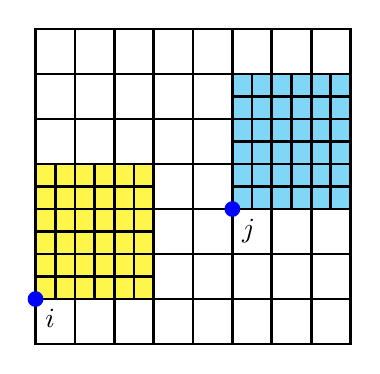
\begin{tikzpicture}[scale=4.0]
    % Define layers
    \pgfdeclarelayer{background}
    \pgfsetlayers{background,main}

    \coordinate (v1_1) at (0.0, 0.0);
    \coordinate (v1_2) at (0.125, 0.0);
    \coordinate (v1_3) at (0.125, 0.14285714285714285);
    \coordinate (v1_4) at (0.0, 0.14285714285714285);
    \draw[black, line width=1.0pt] (v1_1) -- (v1_2) -- (v1_3) -- (v1_4) -- cycle;
    \coordinate (v2_1) at (0.125, 0.0);
    \coordinate (v2_2) at (0.25, 0.0);
    \coordinate (v2_3) at (0.25, 0.14285714285714285);
    \coordinate (v2_4) at (0.125, 0.14285714285714285);
    \draw[black, line width=1.0pt] (v2_1) -- (v2_2) -- (v2_3) -- (v2_4) -- cycle;
    \coordinate (v3_1) at (0.25, 0.0);
    \coordinate (v3_2) at (0.375, 0.0);
    \coordinate (v3_3) at (0.375, 0.14285714285714285);
    \coordinate (v3_4) at (0.25, 0.14285714285714285);
    \draw[black, line width=1.0pt] (v3_1) -- (v3_2) -- (v3_3) -- (v3_4) -- cycle;
    \coordinate (v4_1) at (0.375, 0.0);
    \coordinate (v4_2) at (0.5, 0.0);
    \coordinate (v4_3) at (0.5, 0.14285714285714285);
    \coordinate (v4_4) at (0.375, 0.14285714285714285);
    \draw[black, line width=1.0pt] (v4_1) -- (v4_2) -- (v4_3) -- (v4_4) -- cycle;
    \coordinate (v5_1) at (0.5, 0.0);
    \coordinate (v5_2) at (0.625, 0.0);
    \coordinate (v5_3) at (0.625, 0.14285714285714285);
    \coordinate (v5_4) at (0.5, 0.14285714285714285);
    \draw[black, line width=1.0pt] (v5_1) -- (v5_2) -- (v5_3) -- (v5_4) -- cycle;
    \coordinate (v6_1) at (0.625, 0.0);
    \coordinate (v6_2) at (0.75, 0.0);
    \coordinate (v6_3) at (0.75, 0.14285714285714285);
    \coordinate (v6_4) at (0.625, 0.14285714285714285);
    \draw[black, line width=1.0pt] (v6_1) -- (v6_2) -- (v6_3) -- (v6_4) -- cycle;
    \coordinate (v7_1) at (0.75, 0.0);
    \coordinate (v7_2) at (0.875, 0.0);
    \coordinate (v7_3) at (0.875, 0.14285714285714285);
    \coordinate (v7_4) at (0.75, 0.14285714285714285);
    \draw[black, line width=1.0pt] (v7_1) -- (v7_2) -- (v7_3) -- (v7_4) -- cycle;
    \coordinate (v8_1) at (0.875, 0.0);
    \coordinate (v8_2) at (1.0, 0.0);
    \coordinate (v8_3) at (1.0, 0.14285714285714285);
    \coordinate (v8_4) at (0.875, 0.14285714285714285);
    \draw[black, line width=1.0pt] (v8_1) -- (v8_2) -- (v8_3) -- (v8_4) -- cycle;
    \coordinate (v9_1) at (0.375, 0.14285714285714285);
    \coordinate (v9_2) at (0.5, 0.14285714285714285);
    \coordinate (v9_3) at (0.5, 0.2857142857142857);
    \coordinate (v9_4) at (0.375, 0.2857142857142857);
    \draw[black, line width=1.0pt] (v9_1) -- (v9_2) -- (v9_3) -- (v9_4) -- cycle;
    \coordinate (v10_1) at (0.5, 0.14285714285714285);
    \coordinate (v10_2) at (0.625, 0.14285714285714285);
    \coordinate (v10_3) at (0.625, 0.2857142857142857);
    \coordinate (v10_4) at (0.5, 0.2857142857142857);
    \draw[black, line width=1.0pt] (v10_1) -- (v10_2) -- (v10_3) -- (v10_4) -- cycle;
    \coordinate (v11_1) at (0.625, 0.14285714285714285);
    \coordinate (v11_2) at (0.75, 0.14285714285714285);
    \coordinate (v11_3) at (0.75, 0.2857142857142857);
    \coordinate (v11_4) at (0.625, 0.2857142857142857);
    \draw[black, line width=1.0pt] (v11_1) -- (v11_2) -- (v11_3) -- (v11_4) -- cycle;
    \coordinate (v12_1) at (0.75, 0.14285714285714285);
    \coordinate (v12_2) at (0.875, 0.14285714285714285);
    \coordinate (v12_3) at (0.875, 0.2857142857142857);
    \coordinate (v12_4) at (0.75, 0.2857142857142857);
    \draw[black, line width=1.0pt] (v12_1) -- (v12_2) -- (v12_3) -- (v12_4) -- cycle;
    \coordinate (v13_1) at (0.875, 0.14285714285714285);
    \coordinate (v13_2) at (1.0, 0.14285714285714285);
    \coordinate (v13_3) at (1.0, 0.2857142857142857);
    \coordinate (v13_4) at (0.875, 0.2857142857142857);
    \draw[black, line width=1.0pt] (v13_1) -- (v13_2) -- (v13_3) -- (v13_4) -- cycle;
    \coordinate (v14_1) at (0.375, 0.2857142857142857);
    \coordinate (v14_2) at (0.5, 0.2857142857142857);
    \coordinate (v14_3) at (0.5, 0.42857142857142855);
    \coordinate (v14_4) at (0.375, 0.42857142857142855);
    \draw[black, line width=1.0pt] (v14_1) -- (v14_2) -- (v14_3) -- (v14_4) -- cycle;
    \coordinate (v15_1) at (0.5, 0.2857142857142857);
    \coordinate (v15_2) at (0.625, 0.2857142857142857);
    \coordinate (v15_3) at (0.625, 0.42857142857142855);
    \coordinate (v15_4) at (0.5, 0.42857142857142855);
    \draw[black, line width=1.0pt] (v15_1) -- (v15_2) -- (v15_3) -- (v15_4) -- cycle;
    \coordinate (v16_1) at (0.625, 0.2857142857142857);
    \coordinate (v16_2) at (0.75, 0.2857142857142857);
    \coordinate (v16_3) at (0.75, 0.42857142857142855);
    \coordinate (v16_4) at (0.625, 0.42857142857142855);
    \draw[black, line width=1.0pt] (v16_1) -- (v16_2) -- (v16_3) -- (v16_4) -- cycle;
    \coordinate (v17_1) at (0.75, 0.2857142857142857);
    \coordinate (v17_2) at (0.875, 0.2857142857142857);
    \coordinate (v17_3) at (0.875, 0.42857142857142855);
    \coordinate (v17_4) at (0.75, 0.42857142857142855);
    \draw[black, line width=1.0pt] (v17_1) -- (v17_2) -- (v17_3) -- (v17_4) -- cycle;
    \coordinate (v18_1) at (0.875, 0.2857142857142857);
    \coordinate (v18_2) at (1.0, 0.2857142857142857);
    \coordinate (v18_3) at (1.0, 0.42857142857142855);
    \coordinate (v18_4) at (0.875, 0.42857142857142855);
    \draw[black, line width=1.0pt] (v18_1) -- (v18_2) -- (v18_3) -- (v18_4) -- cycle;
    \coordinate (v19_1) at (0.375, 0.42857142857142855);
    \coordinate (v19_2) at (0.5, 0.42857142857142855);
    \coordinate (v19_3) at (0.5, 0.5714285714285714);
    \coordinate (v19_4) at (0.375, 0.5714285714285714);
    \draw[black, line width=1.0pt] (v19_1) -- (v19_2) -- (v19_3) -- (v19_4) -- cycle;
    \coordinate (v20_1) at (0.5, 0.42857142857142855);
    \coordinate (v20_2) at (0.625, 0.42857142857142855);
    \coordinate (v20_3) at (0.625, 0.5714285714285714);
    \coordinate (v20_4) at (0.5, 0.5714285714285714);
    \draw[black, line width=1.0pt] (v20_1) -- (v20_2) -- (v20_3) -- (v20_4) -- cycle;
    \coordinate (v21_1) at (0.0, 0.5714285714285714);
    \coordinate (v21_2) at (0.125, 0.5714285714285714);
    \coordinate (v21_3) at (0.125, 0.7142857142857143);
    \coordinate (v21_4) at (0.0, 0.7142857142857143);
    \draw[black, line width=1.0pt] (v21_1) -- (v21_2) -- (v21_3) -- (v21_4) -- cycle;
    \coordinate (v22_1) at (0.125, 0.5714285714285714);
    \coordinate (v22_2) at (0.25, 0.5714285714285714);
    \coordinate (v22_3) at (0.25, 0.7142857142857143);
    \coordinate (v22_4) at (0.125, 0.7142857142857143);
    \draw[black, line width=1.0pt] (v22_1) -- (v22_2) -- (v22_3) -- (v22_4) -- cycle;
    \coordinate (v23_1) at (0.25, 0.5714285714285714);
    \coordinate (v23_2) at (0.375, 0.5714285714285714);
    \coordinate (v23_3) at (0.375, 0.7142857142857143);
    \coordinate (v23_4) at (0.25, 0.7142857142857143);
    \draw[black, line width=1.0pt] (v23_1) -- (v23_2) -- (v23_3) -- (v23_4) -- cycle;
    \coordinate (v24_1) at (0.375, 0.5714285714285714);
    \coordinate (v24_2) at (0.5, 0.5714285714285714);
    \coordinate (v24_3) at (0.5, 0.7142857142857143);
    \coordinate (v24_4) at (0.375, 0.7142857142857143);
    \draw[black, line width=1.0pt] (v24_1) -- (v24_2) -- (v24_3) -- (v24_4) -- cycle;
    \coordinate (v25_1) at (0.5, 0.5714285714285714);
    \coordinate (v25_2) at (0.625, 0.5714285714285714);
    \coordinate (v25_3) at (0.625, 0.7142857142857143);
    \coordinate (v25_4) at (0.5, 0.7142857142857143);
    \draw[black, line width=1.0pt] (v25_1) -- (v25_2) -- (v25_3) -- (v25_4) -- cycle;
    \coordinate (v26_1) at (0.0, 0.7142857142857143);
    \coordinate (v26_2) at (0.125, 0.7142857142857143);
    \coordinate (v26_3) at (0.125, 0.8571428571428571);
    \coordinate (v26_4) at (0.0, 0.8571428571428571);
    \draw[black, line width=1.0pt] (v26_1) -- (v26_2) -- (v26_3) -- (v26_4) -- cycle;
    \coordinate (v27_1) at (0.125, 0.7142857142857143);
    \coordinate (v27_2) at (0.25, 0.7142857142857143);
    \coordinate (v27_3) at (0.25, 0.8571428571428571);
    \coordinate (v27_4) at (0.125, 0.8571428571428571);
    \draw[black, line width=1.0pt] (v27_1) -- (v27_2) -- (v27_3) -- (v27_4) -- cycle;
    \coordinate (v28_1) at (0.25, 0.7142857142857143);
    \coordinate (v28_2) at (0.375, 0.7142857142857143);
    \coordinate (v28_3) at (0.375, 0.8571428571428571);
    \coordinate (v28_4) at (0.25, 0.8571428571428571);
    \draw[black, line width=1.0pt] (v28_1) -- (v28_2) -- (v28_3) -- (v28_4) -- cycle;
    \coordinate (v29_1) at (0.375, 0.7142857142857143);
    \coordinate (v29_2) at (0.5, 0.7142857142857143);
    \coordinate (v29_3) at (0.5, 0.8571428571428571);
    \coordinate (v29_4) at (0.375, 0.8571428571428571);
    \draw[black, line width=1.0pt] (v29_1) -- (v29_2) -- (v29_3) -- (v29_4) -- cycle;
    \coordinate (v30_1) at (0.5, 0.7142857142857143);
    \coordinate (v30_2) at (0.625, 0.7142857142857143);
    \coordinate (v30_3) at (0.625, 0.8571428571428571);
    \coordinate (v30_4) at (0.5, 0.8571428571428571);
    \draw[black, line width=1.0pt] (v30_1) -- (v30_2) -- (v30_3) -- (v30_4) -- cycle;
    \coordinate (v31_1) at (0.0, 0.8571428571428571);
    \coordinate (v31_2) at (0.125, 0.8571428571428571);
    \coordinate (v31_3) at (0.125, 1.0);
    \coordinate (v31_4) at (0.0, 1.0);
    \draw[black, line width=1.0pt] (v31_1) -- (v31_2) -- (v31_3) -- (v31_4) -- cycle;
    \coordinate (v32_1) at (0.125, 0.8571428571428571);
    \coordinate (v32_2) at (0.25, 0.8571428571428571);
    \coordinate (v32_3) at (0.25, 1.0);
    \coordinate (v32_4) at (0.125, 1.0);
    \draw[black, line width=1.0pt] (v32_1) -- (v32_2) -- (v32_3) -- (v32_4) -- cycle;
    \coordinate (v33_1) at (0.25, 0.8571428571428571);
    \coordinate (v33_2) at (0.375, 0.8571428571428571);
    \coordinate (v33_3) at (0.375, 1.0);
    \coordinate (v33_4) at (0.25, 1.0);
    \draw[black, line width=1.0pt] (v33_1) -- (v33_2) -- (v33_3) -- (v33_4) -- cycle;
    \coordinate (v34_1) at (0.375, 0.8571428571428571);
    \coordinate (v34_2) at (0.5, 0.8571428571428571);
    \coordinate (v34_3) at (0.5, 1.0);
    \coordinate (v34_4) at (0.375, 1.0);
    \draw[black, line width=1.0pt] (v34_1) -- (v34_2) -- (v34_3) -- (v34_4) -- cycle;
    \coordinate (v35_1) at (0.5, 0.8571428571428571);
    \coordinate (v35_2) at (0.625, 0.8571428571428571);
    \coordinate (v35_3) at (0.625, 1.0);
    \coordinate (v35_4) at (0.5, 1.0);
    \draw[black, line width=1.0pt] (v35_1) -- (v35_2) -- (v35_3) -- (v35_4) -- cycle;
    \coordinate (v36_1) at (0.625, 0.8571428571428571);
    \coordinate (v36_2) at (0.75, 0.8571428571428571);
    \coordinate (v36_3) at (0.75, 1.0);
    \coordinate (v36_4) at (0.625, 1.0);
    \draw[black, line width=1.0pt] (v36_1) -- (v36_2) -- (v36_3) -- (v36_4) -- cycle;
    \coordinate (v37_1) at (0.75, 0.8571428571428571);
    \coordinate (v37_2) at (0.875, 0.8571428571428571);
    \coordinate (v37_3) at (0.875, 1.0);
    \coordinate (v37_4) at (0.75, 1.0);
    \draw[black, line width=1.0pt] (v37_1) -- (v37_2) -- (v37_3) -- (v37_4) -- cycle;
    \coordinate (v38_1) at (0.875, 0.8571428571428571);
    \coordinate (v38_2) at (1.0, 0.8571428571428571);
    \coordinate (v38_3) at (1.0, 1.0);
    \coordinate (v38_4) at (0.875, 1.0);
    \draw[black, line width=1.0pt] (v38_1) -- (v38_2) -- (v38_3) -- (v38_4) -- cycle;
    \coordinate (v39_1) at (0.0, 0.14285714285714285);
    \coordinate (v39_2) at (0.0625, 0.14285714285714285);
    \coordinate (v39_3) at (0.0625, 0.21428571428571427);
    \coordinate (v39_4) at (0.0, 0.21428571428571427);
    \draw[black, line width=1.0pt] (v39_1) -- (v39_2) -- (v39_3) -- (v39_4) -- cycle;
    \coordinate (v40_1) at (0.0625, 0.14285714285714285);
    \coordinate (v40_2) at (0.125, 0.14285714285714285);
    \coordinate (v40_3) at (0.125, 0.21428571428571427);
    \coordinate (v40_4) at (0.0625, 0.21428571428571427);
    \draw[black, line width=1.0pt] (v40_1) -- (v40_2) -- (v40_3) -- (v40_4) -- cycle;
    \coordinate (v41_1) at (0.125, 0.14285714285714285);
    \coordinate (v41_2) at (0.1875, 0.14285714285714285);
    \coordinate (v41_3) at (0.1875, 0.21428571428571427);
    \coordinate (v41_4) at (0.125, 0.21428571428571427);
    \draw[black, line width=1.0pt] (v41_1) -- (v41_2) -- (v41_3) -- (v41_4) -- cycle;
    \coordinate (v42_1) at (0.1875, 0.14285714285714285);
    \coordinate (v42_2) at (0.25, 0.14285714285714285);
    \coordinate (v42_3) at (0.25, 0.21428571428571427);
    \coordinate (v42_4) at (0.1875, 0.21428571428571427);
    \draw[black, line width=1.0pt] (v42_1) -- (v42_2) -- (v42_3) -- (v42_4) -- cycle;
    \coordinate (v43_1) at (0.25, 0.14285714285714285);
    \coordinate (v43_2) at (0.3125, 0.14285714285714285);
    \coordinate (v43_3) at (0.3125, 0.21428571428571427);
    \coordinate (v43_4) at (0.25, 0.21428571428571427);
    \draw[black, line width=1.0pt] (v43_1) -- (v43_2) -- (v43_3) -- (v43_4) -- cycle;
    \coordinate (v44_1) at (0.3125, 0.14285714285714285);
    \coordinate (v44_2) at (0.375, 0.14285714285714285);
    \coordinate (v44_3) at (0.375, 0.21428571428571427);
    \coordinate (v44_4) at (0.3125, 0.21428571428571427);
    \draw[black, line width=1.0pt] (v44_1) -- (v44_2) -- (v44_3) -- (v44_4) -- cycle;
    \coordinate (v45_1) at (0.0, 0.21428571428571427);
    \coordinate (v45_2) at (0.0625, 0.21428571428571427);
    \coordinate (v45_3) at (0.0625, 0.2857142857142857);
    \coordinate (v45_4) at (0.0, 0.2857142857142857);
    \draw[black, line width=1.0pt] (v45_1) -- (v45_2) -- (v45_3) -- (v45_4) -- cycle;
    \coordinate (v46_1) at (0.0625, 0.21428571428571427);
    \coordinate (v46_2) at (0.125, 0.21428571428571427);
    \coordinate (v46_3) at (0.125, 0.2857142857142857);
    \coordinate (v46_4) at (0.0625, 0.2857142857142857);
    \draw[black, line width=1.0pt] (v46_1) -- (v46_2) -- (v46_3) -- (v46_4) -- cycle;
    \coordinate (v47_1) at (0.125, 0.21428571428571427);
    \coordinate (v47_2) at (0.1875, 0.21428571428571427);
    \coordinate (v47_3) at (0.1875, 0.2857142857142857);
    \coordinate (v47_4) at (0.125, 0.2857142857142857);
    \draw[black, line width=1.0pt] (v47_1) -- (v47_2) -- (v47_3) -- (v47_4) -- cycle;
    \coordinate (v48_1) at (0.1875, 0.21428571428571427);
    \coordinate (v48_2) at (0.25, 0.21428571428571427);
    \coordinate (v48_3) at (0.25, 0.2857142857142857);
    \coordinate (v48_4) at (0.1875, 0.2857142857142857);
    \draw[black, line width=1.0pt] (v48_1) -- (v48_2) -- (v48_3) -- (v48_4) -- cycle;
    \coordinate (v49_1) at (0.25, 0.21428571428571427);
    \coordinate (v49_2) at (0.3125, 0.21428571428571427);
    \coordinate (v49_3) at (0.3125, 0.2857142857142857);
    \coordinate (v49_4) at (0.25, 0.2857142857142857);
    \draw[black, line width=1.0pt] (v49_1) -- (v49_2) -- (v49_3) -- (v49_4) -- cycle;
    \coordinate (v50_1) at (0.3125, 0.21428571428571427);
    \coordinate (v50_2) at (0.375, 0.21428571428571427);
    \coordinate (v50_3) at (0.375, 0.2857142857142857);
    \coordinate (v50_4) at (0.3125, 0.2857142857142857);
    \draw[black, line width=1.0pt] (v50_1) -- (v50_2) -- (v50_3) -- (v50_4) -- cycle;
    \coordinate (v51_1) at (0.0, 0.2857142857142857);
    \coordinate (v51_2) at (0.0625, 0.2857142857142857);
    \coordinate (v51_3) at (0.0625, 0.3571428571428571);
    \coordinate (v51_4) at (0.0, 0.3571428571428571);
    \draw[black, line width=1.0pt] (v51_1) -- (v51_2) -- (v51_3) -- (v51_4) -- cycle;
    \coordinate (v52_1) at (0.0625, 0.2857142857142857);
    \coordinate (v52_2) at (0.125, 0.2857142857142857);
    \coordinate (v52_3) at (0.125, 0.3571428571428571);
    \coordinate (v52_4) at (0.0625, 0.3571428571428571);
    \draw[black, line width=1.0pt] (v52_1) -- (v52_2) -- (v52_3) -- (v52_4) -- cycle;
    \coordinate (v53_1) at (0.125, 0.2857142857142857);
    \coordinate (v53_2) at (0.1875, 0.2857142857142857);
    \coordinate (v53_3) at (0.1875, 0.3571428571428571);
    \coordinate (v53_4) at (0.125, 0.3571428571428571);
    \draw[black, line width=1.0pt] (v53_1) -- (v53_2) -- (v53_3) -- (v53_4) -- cycle;
    \coordinate (v54_1) at (0.1875, 0.2857142857142857);
    \coordinate (v54_2) at (0.25, 0.2857142857142857);
    \coordinate (v54_3) at (0.25, 0.3571428571428571);
    \coordinate (v54_4) at (0.1875, 0.3571428571428571);
    \draw[black, line width=1.0pt] (v54_1) -- (v54_2) -- (v54_3) -- (v54_4) -- cycle;
    \coordinate (v55_1) at (0.25, 0.2857142857142857);
    \coordinate (v55_2) at (0.3125, 0.2857142857142857);
    \coordinate (v55_3) at (0.3125, 0.3571428571428571);
    \coordinate (v55_4) at (0.25, 0.3571428571428571);
    \draw[black, line width=1.0pt] (v55_1) -- (v55_2) -- (v55_3) -- (v55_4) -- cycle;
    \coordinate (v56_1) at (0.3125, 0.2857142857142857);
    \coordinate (v56_2) at (0.375, 0.2857142857142857);
    \coordinate (v56_3) at (0.375, 0.3571428571428571);
    \coordinate (v56_4) at (0.3125, 0.3571428571428571);
    \draw[black, line width=1.0pt] (v56_1) -- (v56_2) -- (v56_3) -- (v56_4) -- cycle;
    \coordinate (v57_1) at (0.0, 0.3571428571428571);
    \coordinate (v57_2) at (0.0625, 0.3571428571428571);
    \coordinate (v57_3) at (0.0625, 0.42857142857142855);
    \coordinate (v57_4) at (0.0, 0.42857142857142855);
    \draw[black, line width=1.0pt] (v57_1) -- (v57_2) -- (v57_3) -- (v57_4) -- cycle;
    \coordinate (v58_1) at (0.0625, 0.3571428571428571);
    \coordinate (v58_2) at (0.125, 0.3571428571428571);
    \coordinate (v58_3) at (0.125, 0.42857142857142855);
    \coordinate (v58_4) at (0.0625, 0.42857142857142855);
    \draw[black, line width=1.0pt] (v58_1) -- (v58_2) -- (v58_3) -- (v58_4) -- cycle;
    \coordinate (v59_1) at (0.125, 0.3571428571428571);
    \coordinate (v59_2) at (0.1875, 0.3571428571428571);
    \coordinate (v59_3) at (0.1875, 0.42857142857142855);
    \coordinate (v59_4) at (0.125, 0.42857142857142855);
    \draw[black, line width=1.0pt] (v59_1) -- (v59_2) -- (v59_3) -- (v59_4) -- cycle;
    \coordinate (v60_1) at (0.1875, 0.3571428571428571);
    \coordinate (v60_2) at (0.25, 0.3571428571428571);
    \coordinate (v60_3) at (0.25, 0.42857142857142855);
    \coordinate (v60_4) at (0.1875, 0.42857142857142855);
    \draw[black, line width=1.0pt] (v60_1) -- (v60_2) -- (v60_3) -- (v60_4) -- cycle;
    \coordinate (v61_1) at (0.25, 0.3571428571428571);
    \coordinate (v61_2) at (0.3125, 0.3571428571428571);
    \coordinate (v61_3) at (0.3125, 0.42857142857142855);
    \coordinate (v61_4) at (0.25, 0.42857142857142855);
    \draw[black, line width=1.0pt] (v61_1) -- (v61_2) -- (v61_3) -- (v61_4) -- cycle;
    \coordinate (v62_1) at (0.3125, 0.3571428571428571);
    \coordinate (v62_2) at (0.375, 0.3571428571428571);
    \coordinate (v62_3) at (0.375, 0.42857142857142855);
    \coordinate (v62_4) at (0.3125, 0.42857142857142855);
    \draw[black, line width=1.0pt] (v62_1) -- (v62_2) -- (v62_3) -- (v62_4) -- cycle;
    \coordinate (v63_1) at (0.0, 0.42857142857142855);
    \coordinate (v63_2) at (0.0625, 0.42857142857142855);
    \coordinate (v63_3) at (0.0625, 0.5);
    \coordinate (v63_4) at (0.0, 0.5);
    \draw[black, line width=1.0pt] (v63_1) -- (v63_2) -- (v63_3) -- (v63_4) -- cycle;
    \coordinate (v64_1) at (0.0625, 0.42857142857142855);
    \coordinate (v64_2) at (0.125, 0.42857142857142855);
    \coordinate (v64_3) at (0.125, 0.5);
    \coordinate (v64_4) at (0.0625, 0.5);
    \draw[black, line width=1.0pt] (v64_1) -- (v64_2) -- (v64_3) -- (v64_4) -- cycle;
    \coordinate (v65_1) at (0.125, 0.42857142857142855);
    \coordinate (v65_2) at (0.1875, 0.42857142857142855);
    \coordinate (v65_3) at (0.1875, 0.5);
    \coordinate (v65_4) at (0.125, 0.5);
    \draw[black, line width=1.0pt] (v65_1) -- (v65_2) -- (v65_3) -- (v65_4) -- cycle;
    \coordinate (v66_1) at (0.1875, 0.42857142857142855);
    \coordinate (v66_2) at (0.25, 0.42857142857142855);
    \coordinate (v66_3) at (0.25, 0.5);
    \coordinate (v66_4) at (0.1875, 0.5);
    \draw[black, line width=1.0pt] (v66_1) -- (v66_2) -- (v66_3) -- (v66_4) -- cycle;
    \coordinate (v67_1) at (0.25, 0.42857142857142855);
    \coordinate (v67_2) at (0.3125, 0.42857142857142855);
    \coordinate (v67_3) at (0.3125, 0.5);
    \coordinate (v67_4) at (0.25, 0.5);
    \draw[black, line width=1.0pt] (v67_1) -- (v67_2) -- (v67_3) -- (v67_4) -- cycle;
    \coordinate (v68_1) at (0.3125, 0.42857142857142855);
    \coordinate (v68_2) at (0.375, 0.42857142857142855);
    \coordinate (v68_3) at (0.375, 0.5);
    \coordinate (v68_4) at (0.3125, 0.5);
    \draw[black, line width=1.0pt] (v68_1) -- (v68_2) -- (v68_3) -- (v68_4) -- cycle;
    \coordinate (v69_1) at (0.625, 0.42857142857142855);
    \coordinate (v69_2) at (0.6875, 0.42857142857142855);
    \coordinate (v69_3) at (0.6875, 0.5);
    \coordinate (v69_4) at (0.625, 0.5);
    \draw[black, line width=1.0pt] (v69_1) -- (v69_2) -- (v69_3) -- (v69_4) -- cycle;
    \coordinate (v70_1) at (0.6875, 0.42857142857142855);
    \coordinate (v70_2) at (0.75, 0.42857142857142855);
    \coordinate (v70_3) at (0.75, 0.5);
    \coordinate (v70_4) at (0.6875, 0.5);
    \draw[black, line width=1.0pt] (v70_1) -- (v70_2) -- (v70_3) -- (v70_4) -- cycle;
    \coordinate (v71_1) at (0.75, 0.42857142857142855);
    \coordinate (v71_2) at (0.8125, 0.42857142857142855);
    \coordinate (v71_3) at (0.8125, 0.5);
    \coordinate (v71_4) at (0.75, 0.5);
    \draw[black, line width=1.0pt] (v71_1) -- (v71_2) -- (v71_3) -- (v71_4) -- cycle;
    \coordinate (v72_1) at (0.8125, 0.42857142857142855);
    \coordinate (v72_2) at (0.875, 0.42857142857142855);
    \coordinate (v72_3) at (0.875, 0.5);
    \coordinate (v72_4) at (0.8125, 0.5);
    \draw[black, line width=1.0pt] (v72_1) -- (v72_2) -- (v72_3) -- (v72_4) -- cycle;
    \coordinate (v73_1) at (0.875, 0.42857142857142855);
    \coordinate (v73_2) at (0.9375, 0.42857142857142855);
    \coordinate (v73_3) at (0.9375, 0.5);
    \coordinate (v73_4) at (0.875, 0.5);
    \draw[black, line width=1.0pt] (v73_1) -- (v73_2) -- (v73_3) -- (v73_4) -- cycle;
    \coordinate (v74_1) at (0.9375, 0.42857142857142855);
    \coordinate (v74_2) at (1.0, 0.42857142857142855);
    \coordinate (v74_3) at (1.0, 0.5);
    \coordinate (v74_4) at (0.9375, 0.5);
    \draw[black, line width=1.0pt] (v74_1) -- (v74_2) -- (v74_3) -- (v74_4) -- cycle;
    \coordinate (v75_1) at (0.0, 0.5);
    \coordinate (v75_2) at (0.0625, 0.5);
    \coordinate (v75_3) at (0.0625, 0.5714285714285714);
    \coordinate (v75_4) at (0.0, 0.5714285714285714);
    \draw[black, line width=1.0pt] (v75_1) -- (v75_2) -- (v75_3) -- (v75_4) -- cycle;
    \coordinate (v76_1) at (0.0625, 0.5);
    \coordinate (v76_2) at (0.125, 0.5);
    \coordinate (v76_3) at (0.125, 0.5714285714285714);
    \coordinate (v76_4) at (0.0625, 0.5714285714285714);
    \draw[black, line width=1.0pt] (v76_1) -- (v76_2) -- (v76_3) -- (v76_4) -- cycle;
    \coordinate (v77_1) at (0.125, 0.5);
    \coordinate (v77_2) at (0.1875, 0.5);
    \coordinate (v77_3) at (0.1875, 0.5714285714285714);
    \coordinate (v77_4) at (0.125, 0.5714285714285714);
    \draw[black, line width=1.0pt] (v77_1) -- (v77_2) -- (v77_3) -- (v77_4) -- cycle;
    \coordinate (v78_1) at (0.1875, 0.5);
    \coordinate (v78_2) at (0.25, 0.5);
    \coordinate (v78_3) at (0.25, 0.5714285714285714);
    \coordinate (v78_4) at (0.1875, 0.5714285714285714);
    \draw[black, line width=1.0pt] (v78_1) -- (v78_2) -- (v78_3) -- (v78_4) -- cycle;
    \coordinate (v79_1) at (0.25, 0.5);
    \coordinate (v79_2) at (0.3125, 0.5);
    \coordinate (v79_3) at (0.3125, 0.5714285714285714);
    \coordinate (v79_4) at (0.25, 0.5714285714285714);
    \draw[black, line width=1.0pt] (v79_1) -- (v79_2) -- (v79_3) -- (v79_4) -- cycle;
    \coordinate (v80_1) at (0.3125, 0.5);
    \coordinate (v80_2) at (0.375, 0.5);
    \coordinate (v80_3) at (0.375, 0.5714285714285714);
    \coordinate (v80_4) at (0.3125, 0.5714285714285714);
    \draw[black, line width=1.0pt] (v80_1) -- (v80_2) -- (v80_3) -- (v80_4) -- cycle;
    \coordinate (v81_1) at (0.625, 0.5);
    \coordinate (v81_2) at (0.6875, 0.5);
    \coordinate (v81_3) at (0.6875, 0.5714285714285714);
    \coordinate (v81_4) at (0.625, 0.5714285714285714);
    \draw[black, line width=1.0pt] (v81_1) -- (v81_2) -- (v81_3) -- (v81_4) -- cycle;
    \coordinate (v82_1) at (0.6875, 0.5);
    \coordinate (v82_2) at (0.75, 0.5);
    \coordinate (v82_3) at (0.75, 0.5714285714285714);
    \coordinate (v82_4) at (0.6875, 0.5714285714285714);
    \draw[black, line width=1.0pt] (v82_1) -- (v82_2) -- (v82_3) -- (v82_4) -- cycle;
    \coordinate (v83_1) at (0.75, 0.5);
    \coordinate (v83_2) at (0.8125, 0.5);
    \coordinate (v83_3) at (0.8125, 0.5714285714285714);
    \coordinate (v83_4) at (0.75, 0.5714285714285714);
    \draw[black, line width=1.0pt] (v83_1) -- (v83_2) -- (v83_3) -- (v83_4) -- cycle;
    \coordinate (v84_1) at (0.8125, 0.5);
    \coordinate (v84_2) at (0.875, 0.5);
    \coordinate (v84_3) at (0.875, 0.5714285714285714);
    \coordinate (v84_4) at (0.8125, 0.5714285714285714);
    \draw[black, line width=1.0pt] (v84_1) -- (v84_2) -- (v84_3) -- (v84_4) -- cycle;
    \coordinate (v85_1) at (0.875, 0.5);
    \coordinate (v85_2) at (0.9375, 0.5);
    \coordinate (v85_3) at (0.9375, 0.5714285714285714);
    \coordinate (v85_4) at (0.875, 0.5714285714285714);
    \draw[black, line width=1.0pt] (v85_1) -- (v85_2) -- (v85_3) -- (v85_4) -- cycle;
    \coordinate (v86_1) at (0.9375, 0.5);
    \coordinate (v86_2) at (1.0, 0.5);
    \coordinate (v86_3) at (1.0, 0.5714285714285714);
    \coordinate (v86_4) at (0.9375, 0.5714285714285714);
    \draw[black, line width=1.0pt] (v86_1) -- (v86_2) -- (v86_3) -- (v86_4) -- cycle;
    \coordinate (v87_1) at (0.625, 0.5714285714285714);
    \coordinate (v87_2) at (0.6875, 0.5714285714285714);
    \coordinate (v87_3) at (0.6875, 0.6428571428571428);
    \coordinate (v87_4) at (0.625, 0.6428571428571428);
    \draw[black, line width=1.0pt] (v87_1) -- (v87_2) -- (v87_3) -- (v87_4) -- cycle;
    \coordinate (v88_1) at (0.6875, 0.5714285714285714);
    \coordinate (v88_2) at (0.75, 0.5714285714285714);
    \coordinate (v88_3) at (0.75, 0.6428571428571428);
    \coordinate (v88_4) at (0.6875, 0.6428571428571428);
    \draw[black, line width=1.0pt] (v88_1) -- (v88_2) -- (v88_3) -- (v88_4) -- cycle;
    \coordinate (v89_1) at (0.75, 0.5714285714285714);
    \coordinate (v89_2) at (0.8125, 0.5714285714285714);
    \coordinate (v89_3) at (0.8125, 0.6428571428571428);
    \coordinate (v89_4) at (0.75, 0.6428571428571428);
    \draw[black, line width=1.0pt] (v89_1) -- (v89_2) -- (v89_3) -- (v89_4) -- cycle;
    \coordinate (v90_1) at (0.8125, 0.5714285714285714);
    \coordinate (v90_2) at (0.875, 0.5714285714285714);
    \coordinate (v90_3) at (0.875, 0.6428571428571428);
    \coordinate (v90_4) at (0.8125, 0.6428571428571428);
    \draw[black, line width=1.0pt] (v90_1) -- (v90_2) -- (v90_3) -- (v90_4) -- cycle;
    \coordinate (v91_1) at (0.875, 0.5714285714285714);
    \coordinate (v91_2) at (0.9375, 0.5714285714285714);
    \coordinate (v91_3) at (0.9375, 0.6428571428571428);
    \coordinate (v91_4) at (0.875, 0.6428571428571428);
    \draw[black, line width=1.0pt] (v91_1) -- (v91_2) -- (v91_3) -- (v91_4) -- cycle;
    \coordinate (v92_1) at (0.9375, 0.5714285714285714);
    \coordinate (v92_2) at (1.0, 0.5714285714285714);
    \coordinate (v92_3) at (1.0, 0.6428571428571428);
    \coordinate (v92_4) at (0.9375, 0.6428571428571428);
    \draw[black, line width=1.0pt] (v92_1) -- (v92_2) -- (v92_3) -- (v92_4) -- cycle;
    \coordinate (v93_1) at (0.625, 0.6428571428571428);
    \coordinate (v93_2) at (0.6875, 0.6428571428571428);
    \coordinate (v93_3) at (0.6875, 0.7142857142857143);
    \coordinate (v93_4) at (0.625, 0.7142857142857143);
    \draw[black, line width=1.0pt] (v93_1) -- (v93_2) -- (v93_3) -- (v93_4) -- cycle;
    \coordinate (v94_1) at (0.6875, 0.6428571428571428);
    \coordinate (v94_2) at (0.75, 0.6428571428571428);
    \coordinate (v94_3) at (0.75, 0.7142857142857143);
    \coordinate (v94_4) at (0.6875, 0.7142857142857143);
    \draw[black, line width=1.0pt] (v94_1) -- (v94_2) -- (v94_3) -- (v94_4) -- cycle;
    \coordinate (v95_1) at (0.75, 0.6428571428571428);
    \coordinate (v95_2) at (0.8125, 0.6428571428571428);
    \coordinate (v95_3) at (0.8125, 0.7142857142857143);
    \coordinate (v95_4) at (0.75, 0.7142857142857143);
    \draw[black, line width=1.0pt] (v95_1) -- (v95_2) -- (v95_3) -- (v95_4) -- cycle;
    \coordinate (v96_1) at (0.8125, 0.6428571428571428);
    \coordinate (v96_2) at (0.875, 0.6428571428571428);
    \coordinate (v96_3) at (0.875, 0.7142857142857143);
    \coordinate (v96_4) at (0.8125, 0.7142857142857143);
    \draw[black, line width=1.0pt] (v96_1) -- (v96_2) -- (v96_3) -- (v96_4) -- cycle;
    \coordinate (v97_1) at (0.875, 0.6428571428571428);
    \coordinate (v97_2) at (0.9375, 0.6428571428571428);
    \coordinate (v97_3) at (0.9375, 0.7142857142857143);
    \coordinate (v97_4) at (0.875, 0.7142857142857143);
    \draw[black, line width=1.0pt] (v97_1) -- (v97_2) -- (v97_3) -- (v97_4) -- cycle;
    \coordinate (v98_1) at (0.9375, 0.6428571428571428);
    \coordinate (v98_2) at (1.0, 0.6428571428571428);
    \coordinate (v98_3) at (1.0, 0.7142857142857143);
    \coordinate (v98_4) at (0.9375, 0.7142857142857143);
    \draw[black, line width=1.0pt] (v98_1) -- (v98_2) -- (v98_3) -- (v98_4) -- cycle;
    \coordinate (v99_1) at (0.625, 0.7142857142857143);
    \coordinate (v99_2) at (0.6875, 0.7142857142857143);
    \coordinate (v99_3) at (0.6875, 0.7857142857142857);
    \coordinate (v99_4) at (0.625, 0.7857142857142857);
    \draw[black, line width=1.0pt] (v99_1) -- (v99_2) -- (v99_3) -- (v99_4) -- cycle;
    \coordinate (v100_1) at (0.6875, 0.7142857142857143);
    \coordinate (v100_2) at (0.75, 0.7142857142857143);
    \coordinate (v100_3) at (0.75, 0.7857142857142857);
    \coordinate (v100_4) at (0.6875, 0.7857142857142857);
    \draw[black, line width=1.0pt] (v100_1) -- (v100_2) -- (v100_3) -- (v100_4) -- cycle;
    \coordinate (v101_1) at (0.75, 0.7142857142857143);
    \coordinate (v101_2) at (0.8125, 0.7142857142857143);
    \coordinate (v101_3) at (0.8125, 0.7857142857142857);
    \coordinate (v101_4) at (0.75, 0.7857142857142857);
    \draw[black, line width=1.0pt] (v101_1) -- (v101_2) -- (v101_3) -- (v101_4) -- cycle;
    \coordinate (v102_1) at (0.8125, 0.7142857142857143);
    \coordinate (v102_2) at (0.875, 0.7142857142857143);
    \coordinate (v102_3) at (0.875, 0.7857142857142857);
    \coordinate (v102_4) at (0.8125, 0.7857142857142857);
    \draw[black, line width=1.0pt] (v102_1) -- (v102_2) -- (v102_3) -- (v102_4) -- cycle;
    \coordinate (v103_1) at (0.875, 0.7142857142857143);
    \coordinate (v103_2) at (0.9375, 0.7142857142857143);
    \coordinate (v103_3) at (0.9375, 0.7857142857142857);
    \coordinate (v103_4) at (0.875, 0.7857142857142857);
    \draw[black, line width=1.0pt] (v103_1) -- (v103_2) -- (v103_3) -- (v103_4) -- cycle;
    \coordinate (v104_1) at (0.9375, 0.7142857142857143);
    \coordinate (v104_2) at (1.0, 0.7142857142857143);
    \coordinate (v104_3) at (1.0, 0.7857142857142857);
    \coordinate (v104_4) at (0.9375, 0.7857142857142857);
    \draw[black, line width=1.0pt] (v104_1) -- (v104_2) -- (v104_3) -- (v104_4) -- cycle;
    \coordinate (v105_1) at (0.625, 0.7857142857142857);
    \coordinate (v105_2) at (0.6875, 0.7857142857142857);
    \coordinate (v105_3) at (0.6875, 0.8571428571428571);
    \coordinate (v105_4) at (0.625, 0.8571428571428571);
    \draw[black, line width=1.0pt] (v105_1) -- (v105_2) -- (v105_3) -- (v105_4) -- cycle;
    \coordinate (v106_1) at (0.6875, 0.7857142857142857);
    \coordinate (v106_2) at (0.75, 0.7857142857142857);
    \coordinate (v106_3) at (0.75, 0.8571428571428571);
    \coordinate (v106_4) at (0.6875, 0.8571428571428571);
    \draw[black, line width=1.0pt] (v106_1) -- (v106_2) -- (v106_3) -- (v106_4) -- cycle;
    \coordinate (v107_1) at (0.75, 0.7857142857142857);
    \coordinate (v107_2) at (0.8125, 0.7857142857142857);
    \coordinate (v107_3) at (0.8125, 0.8571428571428571);
    \coordinate (v107_4) at (0.75, 0.8571428571428571);
    \draw[black, line width=1.0pt] (v107_1) -- (v107_2) -- (v107_3) -- (v107_4) -- cycle;
    \coordinate (v108_1) at (0.8125, 0.7857142857142857);
    \coordinate (v108_2) at (0.875, 0.7857142857142857);
    \coordinate (v108_3) at (0.875, 0.8571428571428571);
    \coordinate (v108_4) at (0.8125, 0.8571428571428571);
    \draw[black, line width=1.0pt] (v108_1) -- (v108_2) -- (v108_3) -- (v108_4) -- cycle;
    \coordinate (v109_1) at (0.875, 0.7857142857142857);
    \coordinate (v109_2) at (0.9375, 0.7857142857142857);
    \coordinate (v109_3) at (0.9375, 0.8571428571428571);
    \coordinate (v109_4) at (0.875, 0.8571428571428571);
    \draw[black, line width=1.0pt] (v109_1) -- (v109_2) -- (v109_3) -- (v109_4) -- cycle;
    \coordinate (v110_1) at (0.9375, 0.7857142857142857);
    \coordinate (v110_2) at (1.0, 0.7857142857142857);
    \coordinate (v110_3) at (1.0, 0.8571428571428571);
    \coordinate (v110_4) at (0.9375, 0.8571428571428571);
    \draw[black, line width=1.0pt] (v110_1) -- (v110_2) -- (v110_3) -- (v110_4) -- cycle;

    % Fill the pair support
    \begin{pgfonlayer}{background}
        \fill[yellow, opacity=0.7] (v1_4) rectangle (v19_4);
        \fill[cyan, opacity=0.5] (v20_2) rectangle (v38_2);
    \end{pgfonlayer}

    \node[anchor=north west] at (v1_4) {\(\boldvec{i}\)};
    \node[anchor=north west] at (v20_2) {\(\boldvec{j}\)};
    
    \fill[blue] (v1_4) circle (0.025);
    \fill[blue] (v20_2) circle (0.025);
\end{tikzpicture}

        \caption{}
        \label{fig:problematic-pair-algorithm-case-1-illustration}
    \end{subfigure}
	\hfill
    \begin{subfigure}[t]{0.325\textwidth}
		\centering
		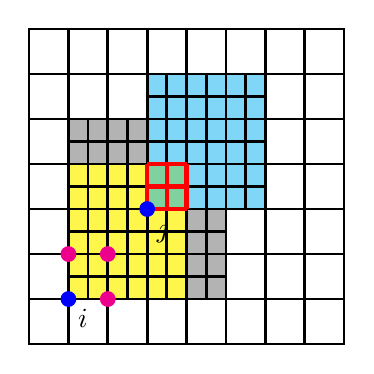
\begin{tikzpicture}[scale=4.0]
    % Define layers
    \pgfdeclarelayer{background}
    \pgfsetlayers{background,main}
    
    \coordinate (v1_1) at (0.0, 0.0);
    \coordinate (v1_2) at (0.125, 0.0);
    \coordinate (v1_3) at (0.125, 0.14285714285714285);
    \coordinate (v1_4) at (0.0, 0.14285714285714285);
    \draw[black, line width=1.0pt] (v1_1) -- (v1_2) -- (v1_3) -- (v1_4) -- cycle;
    \coordinate (v2_1) at (0.125, 0.0);
    \coordinate (v2_2) at (0.25, 0.0);
    \coordinate (v2_3) at (0.25, 0.14285714285714285);
    \coordinate (v2_4) at (0.125, 0.14285714285714285);
    \draw[black, line width=1.0pt] (v2_1) -- (v2_2) -- (v2_3) -- (v2_4) -- cycle;
    \coordinate (v3_1) at (0.25, 0.0);
    \coordinate (v3_2) at (0.375, 0.0);
    \coordinate (v3_3) at (0.375, 0.14285714285714285);
    \coordinate (v3_4) at (0.25, 0.14285714285714285);
    \draw[black, line width=1.0pt] (v3_1) -- (v3_2) -- (v3_3) -- (v3_4) -- cycle;
    \coordinate (v4_1) at (0.375, 0.0);
    \coordinate (v4_2) at (0.5, 0.0);
    \coordinate (v4_3) at (0.5, 0.14285714285714285);
    \coordinate (v4_4) at (0.375, 0.14285714285714285);
    \draw[black, line width=1.0pt] (v4_1) -- (v4_2) -- (v4_3) -- (v4_4) -- cycle;
    \coordinate (v5_1) at (0.5, 0.0);
    \coordinate (v5_2) at (0.625, 0.0);
    \coordinate (v5_3) at (0.625, 0.14285714285714285);
    \coordinate (v5_4) at (0.5, 0.14285714285714285);
    \draw[black, line width=1.0pt] (v5_1) -- (v5_2) -- (v5_3) -- (v5_4) -- cycle;
    \coordinate (v6_1) at (0.625, 0.0);
    \coordinate (v6_2) at (0.75, 0.0);
    \coordinate (v6_3) at (0.75, 0.14285714285714285);
    \coordinate (v6_4) at (0.625, 0.14285714285714285);
    \draw[black, line width=1.0pt] (v6_1) -- (v6_2) -- (v6_3) -- (v6_4) -- cycle;
    \coordinate (v7_1) at (0.75, 0.0);
    \coordinate (v7_2) at (0.875, 0.0);
    \coordinate (v7_3) at (0.875, 0.14285714285714285);
    \coordinate (v7_4) at (0.75, 0.14285714285714285);
    \draw[black, line width=1.0pt] (v7_1) -- (v7_2) -- (v7_3) -- (v7_4) -- cycle;
    \coordinate (v8_1) at (0.875, 0.0);
    \coordinate (v8_2) at (1.0, 0.0);
    \coordinate (v8_3) at (1.0, 0.14285714285714285);
    \coordinate (v8_4) at (0.875, 0.14285714285714285);
    \draw[black, line width=1.0pt] (v8_1) -- (v8_2) -- (v8_3) -- (v8_4) -- cycle;
    \coordinate (v9_1) at (0.0, 0.14285714285714285);
    \coordinate (v9_2) at (0.125, 0.14285714285714285);
    \coordinate (v9_3) at (0.125, 0.2857142857142857);
    \coordinate (v9_4) at (0.0, 0.2857142857142857);
    \draw[black, line width=1.0pt] (v9_1) -- (v9_2) -- (v9_3) -- (v9_4) -- cycle;
    \coordinate (v10_1) at (0.625, 0.14285714285714285);
    \coordinate (v10_2) at (0.75, 0.14285714285714285);
    \coordinate (v10_3) at (0.75, 0.2857142857142857);
    \coordinate (v10_4) at (0.625, 0.2857142857142857);
    \draw[black, line width=1.0pt] (v10_1) -- (v10_2) -- (v10_3) -- (v10_4) -- cycle;
    \coordinate (v11_1) at (0.75, 0.14285714285714285);
    \coordinate (v11_2) at (0.875, 0.14285714285714285);
    \coordinate (v11_3) at (0.875, 0.2857142857142857);
    \coordinate (v11_4) at (0.75, 0.2857142857142857);
    \draw[black, line width=1.0pt] (v11_1) -- (v11_2) -- (v11_3) -- (v11_4) -- cycle;
    \coordinate (v12_1) at (0.875, 0.14285714285714285);
    \coordinate (v12_2) at (1.0, 0.14285714285714285);
    \coordinate (v12_3) at (1.0, 0.2857142857142857);
    \coordinate (v12_4) at (0.875, 0.2857142857142857);
    \draw[black, line width=1.0pt] (v12_1) -- (v12_2) -- (v12_3) -- (v12_4) -- cycle;
    \coordinate (v13_1) at (0.0, 0.2857142857142857);
    \coordinate (v13_2) at (0.125, 0.2857142857142857);
    \coordinate (v13_3) at (0.125, 0.42857142857142855);
    \coordinate (v13_4) at (0.0, 0.42857142857142855);
    \draw[black, line width=1.0pt] (v13_1) -- (v13_2) -- (v13_3) -- (v13_4) -- cycle;
    \coordinate (v14_1) at (0.625, 0.2857142857142857);
    \coordinate (v14_2) at (0.75, 0.2857142857142857);
    \coordinate (v14_3) at (0.75, 0.42857142857142855);
    \coordinate (v14_4) at (0.625, 0.42857142857142855);
    \draw[black, line width=1.0pt] (v14_1) -- (v14_2) -- (v14_3) -- (v14_4) -- cycle;
    \coordinate (v15_1) at (0.75, 0.2857142857142857);
    \coordinate (v15_2) at (0.875, 0.2857142857142857);
    \coordinate (v15_3) at (0.875, 0.42857142857142855);
    \coordinate (v15_4) at (0.75, 0.42857142857142855);
    \draw[black, line width=1.0pt] (v15_1) -- (v15_2) -- (v15_3) -- (v15_4) -- cycle;
    \coordinate (v16_1) at (0.875, 0.2857142857142857);
    \coordinate (v16_2) at (1.0, 0.2857142857142857);
    \coordinate (v16_3) at (1.0, 0.42857142857142855);
    \coordinate (v16_4) at (0.875, 0.42857142857142855);
    \draw[black, line width=1.0pt] (v16_1) -- (v16_2) -- (v16_3) -- (v16_4) -- cycle;
    \coordinate (v17_1) at (0.0, 0.42857142857142855);
    \coordinate (v17_2) at (0.125, 0.42857142857142855);
    \coordinate (v17_3) at (0.125, 0.5714285714285714);
    \coordinate (v17_4) at (0.0, 0.5714285714285714);
    \draw[black, line width=1.0pt] (v17_1) -- (v17_2) -- (v17_3) -- (v17_4) -- cycle;
    \coordinate (v18_1) at (0.75, 0.42857142857142855);
    \coordinate (v18_2) at (0.875, 0.42857142857142855);
    \coordinate (v18_3) at (0.875, 0.5714285714285714);
    \coordinate (v18_4) at (0.75, 0.5714285714285714);
    \draw[black, line width=1.0pt] (v18_1) -- (v18_2) -- (v18_3) -- (v18_4) -- cycle;
    \coordinate (v19_1) at (0.875, 0.42857142857142855);
    \coordinate (v19_2) at (1.0, 0.42857142857142855);
    \coordinate (v19_3) at (1.0, 0.5714285714285714);
    \coordinate (v19_4) at (0.875, 0.5714285714285714);
    \draw[black, line width=1.0pt] (v19_1) -- (v19_2) -- (v19_3) -- (v19_4) -- cycle;
    \coordinate (v20_1) at (0.0, 0.5714285714285714);
    \coordinate (v20_2) at (0.125, 0.5714285714285714);
    \coordinate (v20_3) at (0.125, 0.7142857142857143);
    \coordinate (v20_4) at (0.0, 0.7142857142857143);
    \draw[black, line width=1.0pt] (v20_1) -- (v20_2) -- (v20_3) -- (v20_4) -- cycle;
    \coordinate (v21_1) at (0.75, 0.5714285714285714);
    \coordinate (v21_2) at (0.875, 0.5714285714285714);
    \coordinate (v21_3) at (0.875, 0.7142857142857143);
    \coordinate (v21_4) at (0.75, 0.7142857142857143);
    \draw[black, line width=1.0pt] (v21_1) -- (v21_2) -- (v21_3) -- (v21_4) -- cycle;
    \coordinate (v22_1) at (0.875, 0.5714285714285714);
    \coordinate (v22_2) at (1.0, 0.5714285714285714);
    \coordinate (v22_3) at (1.0, 0.7142857142857143);
    \coordinate (v22_4) at (0.875, 0.7142857142857143);
    \draw[black, line width=1.0pt] (v22_1) -- (v22_2) -- (v22_3) -- (v22_4) -- cycle;
    \coordinate (v23_1) at (0.0, 0.7142857142857143);
    \coordinate (v23_2) at (0.125, 0.7142857142857143);
    \coordinate (v23_3) at (0.125, 0.8571428571428571);
    \coordinate (v23_4) at (0.0, 0.8571428571428571);
    \draw[black, line width=1.0pt] (v23_1) -- (v23_2) -- (v23_3) -- (v23_4) -- cycle;
    \coordinate (v24_1) at (0.125, 0.7142857142857143);
    \coordinate (v24_2) at (0.25, 0.7142857142857143);
    \coordinate (v24_3) at (0.25, 0.8571428571428571);
    \coordinate (v24_4) at (0.125, 0.8571428571428571);
    \draw[black, line width=1.0pt] (v24_1) -- (v24_2) -- (v24_3) -- (v24_4) -- cycle;
    \coordinate (v25_1) at (0.25, 0.7142857142857143);
    \coordinate (v25_2) at (0.375, 0.7142857142857143);
    \coordinate (v25_3) at (0.375, 0.8571428571428571);
    \coordinate (v25_4) at (0.25, 0.8571428571428571);
    \draw[black, line width=1.0pt] (v25_1) -- (v25_2) -- (v25_3) -- (v25_4) -- cycle;
    \coordinate (v26_1) at (0.75, 0.7142857142857143);
    \coordinate (v26_2) at (0.875, 0.7142857142857143);
    \coordinate (v26_3) at (0.875, 0.8571428571428571);
    \coordinate (v26_4) at (0.75, 0.8571428571428571);
    \draw[black, line width=1.0pt] (v26_1) -- (v26_2) -- (v26_3) -- (v26_4) -- cycle;
    \coordinate (v27_1) at (0.875, 0.7142857142857143);
    \coordinate (v27_2) at (1.0, 0.7142857142857143);
    \coordinate (v27_3) at (1.0, 0.8571428571428571);
    \coordinate (v27_4) at (0.875, 0.8571428571428571);
    \draw[black, line width=1.0pt] (v27_1) -- (v27_2) -- (v27_3) -- (v27_4) -- cycle;
    \coordinate (v28_1) at (0.0, 0.8571428571428571);
    \coordinate (v28_2) at (0.125, 0.8571428571428571);
    \coordinate (v28_3) at (0.125, 1.0);
    \coordinate (v28_4) at (0.0, 1.0);
    \draw[black, line width=1.0pt] (v28_1) -- (v28_2) -- (v28_3) -- (v28_4) -- cycle;
    \coordinate (v29_1) at (0.125, 0.8571428571428571);
    \coordinate (v29_2) at (0.25, 0.8571428571428571);
    \coordinate (v29_3) at (0.25, 1.0);
    \coordinate (v29_4) at (0.125, 1.0);
    \draw[black, line width=1.0pt] (v29_1) -- (v29_2) -- (v29_3) -- (v29_4) -- cycle;
    \coordinate (v30_1) at (0.25, 0.8571428571428571);
    \coordinate (v30_2) at (0.375, 0.8571428571428571);
    \coordinate (v30_3) at (0.375, 1.0);
    \coordinate (v30_4) at (0.25, 1.0);
    \draw[black, line width=1.0pt] (v30_1) -- (v30_2) -- (v30_3) -- (v30_4) -- cycle;
    \coordinate (v31_1) at (0.375, 0.8571428571428571);
    \coordinate (v31_2) at (0.5, 0.8571428571428571);
    \coordinate (v31_3) at (0.5, 1.0);
    \coordinate (v31_4) at (0.375, 1.0);
    \draw[black, line width=1.0pt] (v31_1) -- (v31_2) -- (v31_3) -- (v31_4) -- cycle;
    \coordinate (v32_1) at (0.5, 0.8571428571428571);
    \coordinate (v32_2) at (0.625, 0.8571428571428571);
    \coordinate (v32_3) at (0.625, 1.0);
    \coordinate (v32_4) at (0.5, 1.0);
    \draw[black, line width=1.0pt] (v32_1) -- (v32_2) -- (v32_3) -- (v32_4) -- cycle;
    \coordinate (v33_1) at (0.625, 0.8571428571428571);
    \coordinate (v33_2) at (0.75, 0.8571428571428571);
    \coordinate (v33_3) at (0.75, 1.0);
    \coordinate (v33_4) at (0.625, 1.0);
    \draw[black, line width=1.0pt] (v33_1) -- (v33_2) -- (v33_3) -- (v33_4) -- cycle;
    \coordinate (v34_1) at (0.75, 0.8571428571428571);
    \coordinate (v34_2) at (0.875, 0.8571428571428571);
    \coordinate (v34_3) at (0.875, 1.0);
    \coordinate (v34_4) at (0.75, 1.0);
    \draw[black, line width=1.0pt] (v34_1) -- (v34_2) -- (v34_3) -- (v34_4) -- cycle;
    \coordinate (v35_1) at (0.875, 0.8571428571428571);
    \coordinate (v35_2) at (1.0, 0.8571428571428571);
    \coordinate (v35_3) at (1.0, 1.0);
    \coordinate (v35_4) at (0.875, 1.0);
    \draw[black, line width=1.0pt] (v35_1) -- (v35_2) -- (v35_3) -- (v35_4) -- cycle;
    \coordinate (v36_1) at (0.125, 0.14285714285714285);
    \coordinate (v36_2) at (0.1875, 0.14285714285714285);
    \coordinate (v36_3) at (0.1875, 0.21428571428571427);
    \coordinate (v36_4) at (0.125, 0.21428571428571427);
    \draw[black, line width=1.0pt] (v36_1) -- (v36_2) -- (v36_3) -- (v36_4) -- cycle;
    \coordinate (v37_1) at (0.1875, 0.14285714285714285);
    \coordinate (v37_2) at (0.25, 0.14285714285714285);
    \coordinate (v37_3) at (0.25, 0.21428571428571427);
    \coordinate (v37_4) at (0.1875, 0.21428571428571427);
    \draw[black, line width=1.0pt] (v37_1) -- (v37_2) -- (v37_3) -- (v37_4) -- cycle;
    \coordinate (v38_1) at (0.25, 0.14285714285714285);
    \coordinate (v38_2) at (0.3125, 0.14285714285714285);
    \coordinate (v38_3) at (0.3125, 0.21428571428571427);
    \coordinate (v38_4) at (0.25, 0.21428571428571427);
    \draw[black, line width=1.0pt] (v38_1) -- (v38_2) -- (v38_3) -- (v38_4) -- cycle;
    \coordinate (v39_1) at (0.3125, 0.14285714285714285);
    \coordinate (v39_2) at (0.375, 0.14285714285714285);
    \coordinate (v39_3) at (0.375, 0.21428571428571427);
    \coordinate (v39_4) at (0.3125, 0.21428571428571427);
    \draw[black, line width=1.0pt] (v39_1) -- (v39_2) -- (v39_3) -- (v39_4) -- cycle;
    \coordinate (v40_1) at (0.375, 0.14285714285714285);
    \coordinate (v40_2) at (0.4375, 0.14285714285714285);
    \coordinate (v40_3) at (0.4375, 0.21428571428571427);
    \coordinate (v40_4) at (0.375, 0.21428571428571427);
    \draw[black, line width=1.0pt] (v40_1) -- (v40_2) -- (v40_3) -- (v40_4) -- cycle;
    \coordinate (v41_1) at (0.4375, 0.14285714285714285);
    \coordinate (v41_2) at (0.5, 0.14285714285714285);
    \coordinate (v41_3) at (0.5, 0.21428571428571427);
    \coordinate (v41_4) at (0.4375, 0.21428571428571427);
    \draw[black, line width=1.0pt] (v41_1) -- (v41_2) -- (v41_3) -- (v41_4) -- cycle;
    \coordinate (v42_1) at (0.5, 0.14285714285714285);
    \coordinate (v42_2) at (0.5625, 0.14285714285714285);
    \coordinate (v42_3) at (0.5625, 0.21428571428571427);
    \coordinate (v42_4) at (0.5, 0.21428571428571427);
    \draw[black, line width=1.0pt] (v42_1) -- (v42_2) -- (v42_3) -- (v42_4) -- cycle;
    \coordinate (v43_1) at (0.5625, 0.14285714285714285);
    \coordinate (v43_2) at (0.625, 0.14285714285714285);
    \coordinate (v43_3) at (0.625, 0.21428571428571427);
    \coordinate (v43_4) at (0.5625, 0.21428571428571427);
    \draw[black, line width=1.0pt] (v43_1) -- (v43_2) -- (v43_3) -- (v43_4) -- cycle;
    \coordinate (v44_1) at (0.125, 0.21428571428571427);
    \coordinate (v44_2) at (0.1875, 0.21428571428571427);
    \coordinate (v44_3) at (0.1875, 0.2857142857142857);
    \coordinate (v44_4) at (0.125, 0.2857142857142857);
    \draw[black, line width=1.0pt] (v44_1) -- (v44_2) -- (v44_3) -- (v44_4) -- cycle;
    \coordinate (v45_1) at (0.1875, 0.21428571428571427);
    \coordinate (v45_2) at (0.25, 0.21428571428571427);
    \coordinate (v45_3) at (0.25, 0.2857142857142857);
    \coordinate (v45_4) at (0.1875, 0.2857142857142857);
    \draw[black, line width=1.0pt] (v45_1) -- (v45_2) -- (v45_3) -- (v45_4) -- cycle;
    \coordinate (v46_1) at (0.25, 0.21428571428571427);
    \coordinate (v46_2) at (0.3125, 0.21428571428571427);
    \coordinate (v46_3) at (0.3125, 0.2857142857142857);
    \coordinate (v46_4) at (0.25, 0.2857142857142857);
    \draw[black, line width=1.0pt] (v46_1) -- (v46_2) -- (v46_3) -- (v46_4) -- cycle;
    \coordinate (v47_1) at (0.3125, 0.21428571428571427);
    \coordinate (v47_2) at (0.375, 0.21428571428571427);
    \coordinate (v47_3) at (0.375, 0.2857142857142857);
    \coordinate (v47_4) at (0.3125, 0.2857142857142857);
    \draw[black, line width=1.0pt] (v47_1) -- (v47_2) -- (v47_3) -- (v47_4) -- cycle;
    \coordinate (v48_1) at (0.375, 0.21428571428571427);
    \coordinate (v48_2) at (0.4375, 0.21428571428571427);
    \coordinate (v48_3) at (0.4375, 0.2857142857142857);
    \coordinate (v48_4) at (0.375, 0.2857142857142857);
    \draw[black, line width=1.0pt] (v48_1) -- (v48_2) -- (v48_3) -- (v48_4) -- cycle;
    \coordinate (v49_1) at (0.4375, 0.21428571428571427);
    \coordinate (v49_2) at (0.5, 0.21428571428571427);
    \coordinate (v49_3) at (0.5, 0.2857142857142857);
    \coordinate (v49_4) at (0.4375, 0.2857142857142857);
    \draw[black, line width=1.0pt] (v49_1) -- (v49_2) -- (v49_3) -- (v49_4) -- cycle;
    \coordinate (v50_1) at (0.5, 0.21428571428571427);
    \coordinate (v50_2) at (0.5625, 0.21428571428571427);
    \coordinate (v50_3) at (0.5625, 0.2857142857142857);
    \coordinate (v50_4) at (0.5, 0.2857142857142857);
    \draw[black, line width=1.0pt] (v50_1) -- (v50_2) -- (v50_3) -- (v50_4) -- cycle;
    \coordinate (v51_1) at (0.5625, 0.21428571428571427);
    \coordinate (v51_2) at (0.625, 0.21428571428571427);
    \coordinate (v51_3) at (0.625, 0.2857142857142857);
    \coordinate (v51_4) at (0.5625, 0.2857142857142857);
    \draw[black, line width=1.0pt] (v51_1) -- (v51_2) -- (v51_3) -- (v51_4) -- cycle;
    \coordinate (v52_1) at (0.125, 0.2857142857142857);
    \coordinate (v52_2) at (0.1875, 0.2857142857142857);
    \coordinate (v52_3) at (0.1875, 0.3571428571428571);
    \coordinate (v52_4) at (0.125, 0.3571428571428571);
    \draw[black, line width=1.0pt] (v52_1) -- (v52_2) -- (v52_3) -- (v52_4) -- cycle;
    \coordinate (v53_1) at (0.1875, 0.2857142857142857);
    \coordinate (v53_2) at (0.25, 0.2857142857142857);
    \coordinate (v53_3) at (0.25, 0.3571428571428571);
    \coordinate (v53_4) at (0.1875, 0.3571428571428571);
    \draw[black, line width=1.0pt] (v53_1) -- (v53_2) -- (v53_3) -- (v53_4) -- cycle;
    \coordinate (v54_1) at (0.25, 0.2857142857142857);
    \coordinate (v54_2) at (0.3125, 0.2857142857142857);
    \coordinate (v54_3) at (0.3125, 0.3571428571428571);
    \coordinate (v54_4) at (0.25, 0.3571428571428571);
    \draw[black, line width=1.0pt] (v54_1) -- (v54_2) -- (v54_3) -- (v54_4) -- cycle;
    \coordinate (v55_1) at (0.3125, 0.2857142857142857);
    \coordinate (v55_2) at (0.375, 0.2857142857142857);
    \coordinate (v55_3) at (0.375, 0.3571428571428571);
    \coordinate (v55_4) at (0.3125, 0.3571428571428571);
    \draw[black, line width=1.0pt] (v55_1) -- (v55_2) -- (v55_3) -- (v55_4) -- cycle;
    \coordinate (v56_1) at (0.375, 0.2857142857142857);
    \coordinate (v56_2) at (0.4375, 0.2857142857142857);
    \coordinate (v56_3) at (0.4375, 0.3571428571428571);
    \coordinate (v56_4) at (0.375, 0.3571428571428571);
    \draw[black, line width=1.0pt] (v56_1) -- (v56_2) -- (v56_3) -- (v56_4) -- cycle;
    \coordinate (v57_1) at (0.4375, 0.2857142857142857);
    \coordinate (v57_2) at (0.5, 0.2857142857142857);
    \coordinate (v57_3) at (0.5, 0.3571428571428571);
    \coordinate (v57_4) at (0.4375, 0.3571428571428571);
    \draw[black, line width=1.0pt] (v57_1) -- (v57_2) -- (v57_3) -- (v57_4) -- cycle;
    \coordinate (v58_1) at (0.5, 0.2857142857142857);
    \coordinate (v58_2) at (0.5625, 0.2857142857142857);
    \coordinate (v58_3) at (0.5625, 0.3571428571428571);
    \coordinate (v58_4) at (0.5, 0.3571428571428571);
    \draw[black, line width=1.0pt] (v58_1) -- (v58_2) -- (v58_3) -- (v58_4) -- cycle;
    \coordinate (v59_1) at (0.5625, 0.2857142857142857);
    \coordinate (v59_2) at (0.625, 0.2857142857142857);
    \coordinate (v59_3) at (0.625, 0.3571428571428571);
    \coordinate (v59_4) at (0.5625, 0.3571428571428571);
    \draw[black, line width=1.0pt] (v59_1) -- (v59_2) -- (v59_3) -- (v59_4) -- cycle;
    \coordinate (v60_1) at (0.125, 0.3571428571428571);
    \coordinate (v60_2) at (0.1875, 0.3571428571428571);
    \coordinate (v60_3) at (0.1875, 0.42857142857142855);
    \coordinate (v60_4) at (0.125, 0.42857142857142855);
    \draw[black, line width=1.0pt] (v60_1) -- (v60_2) -- (v60_3) -- (v60_4) -- cycle;
    \coordinate (v61_1) at (0.1875, 0.3571428571428571);
    \coordinate (v61_2) at (0.25, 0.3571428571428571);
    \coordinate (v61_3) at (0.25, 0.42857142857142855);
    \coordinate (v61_4) at (0.1875, 0.42857142857142855);
    \draw[black, line width=1.0pt] (v61_1) -- (v61_2) -- (v61_3) -- (v61_4) -- cycle;
    \coordinate (v62_1) at (0.25, 0.3571428571428571);
    \coordinate (v62_2) at (0.3125, 0.3571428571428571);
    \coordinate (v62_3) at (0.3125, 0.42857142857142855);
    \coordinate (v62_4) at (0.25, 0.42857142857142855);
    \draw[black, line width=1.0pt] (v62_1) -- (v62_2) -- (v62_3) -- (v62_4) -- cycle;
    \coordinate (v63_1) at (0.3125, 0.3571428571428571);
    \coordinate (v63_2) at (0.375, 0.3571428571428571);
    \coordinate (v63_3) at (0.375, 0.42857142857142855);
    \coordinate (v63_4) at (0.3125, 0.42857142857142855);
    \draw[black, line width=1.0pt] (v63_1) -- (v63_2) -- (v63_3) -- (v63_4) -- cycle;
    \coordinate (v64_1) at (0.375, 0.3571428571428571);
    \coordinate (v64_2) at (0.4375, 0.3571428571428571);
    \coordinate (v64_3) at (0.4375, 0.42857142857142855);
    \coordinate (v64_4) at (0.375, 0.42857142857142855);
    \draw[black, line width=1.0pt] (v64_1) -- (v64_2) -- (v64_3) -- (v64_4) -- cycle;
    \coordinate (v65_1) at (0.4375, 0.3571428571428571);
    \coordinate (v65_2) at (0.5, 0.3571428571428571);
    \coordinate (v65_3) at (0.5, 0.42857142857142855);
    \coordinate (v65_4) at (0.4375, 0.42857142857142855);
    \draw[black, line width=1.0pt] (v65_1) -- (v65_2) -- (v65_3) -- (v65_4) -- cycle;
    \coordinate (v66_1) at (0.5, 0.3571428571428571);
    \coordinate (v66_2) at (0.5625, 0.3571428571428571);
    \coordinate (v66_3) at (0.5625, 0.42857142857142855);
    \coordinate (v66_4) at (0.5, 0.42857142857142855);
    \draw[black, line width=1.0pt] (v66_1) -- (v66_2) -- (v66_3) -- (v66_4) -- cycle;
    \coordinate (v67_1) at (0.5625, 0.3571428571428571);
    \coordinate (v67_2) at (0.625, 0.3571428571428571);
    \coordinate (v67_3) at (0.625, 0.42857142857142855);
    \coordinate (v67_4) at (0.5625, 0.42857142857142855);
    \draw[black, line width=1.0pt] (v67_1) -- (v67_2) -- (v67_3) -- (v67_4) -- cycle;
    \coordinate (v68_1) at (0.125, 0.42857142857142855);
    \coordinate (v68_2) at (0.1875, 0.42857142857142855);
    \coordinate (v68_3) at (0.1875, 0.5);
    \coordinate (v68_4) at (0.125, 0.5);
    \draw[black, line width=1.0pt] (v68_1) -- (v68_2) -- (v68_3) -- (v68_4) -- cycle;
    \coordinate (v69_1) at (0.1875, 0.42857142857142855);
    \coordinate (v69_2) at (0.25, 0.42857142857142855);
    \coordinate (v69_3) at (0.25, 0.5);
    \coordinate (v69_4) at (0.1875, 0.5);
    \draw[black, line width=1.0pt] (v69_1) -- (v69_2) -- (v69_3) -- (v69_4) -- cycle;
    \coordinate (v70_1) at (0.25, 0.42857142857142855);
    \coordinate (v70_2) at (0.3125, 0.42857142857142855);
    \coordinate (v70_3) at (0.3125, 0.5);
    \coordinate (v70_4) at (0.25, 0.5);
    \draw[black, line width=1.0pt] (v70_1) -- (v70_2) -- (v70_3) -- (v70_4) -- cycle;
    \coordinate (v71_1) at (0.3125, 0.42857142857142855);
    \coordinate (v71_2) at (0.375, 0.42857142857142855);
    \coordinate (v71_3) at (0.375, 0.5);
    \coordinate (v71_4) at (0.3125, 0.5);
    \draw[black, line width=1.0pt] (v71_1) -- (v71_2) -- (v71_3) -- (v71_4) -- cycle;
    \coordinate (v72_1) at (0.375, 0.42857142857142855);
    \coordinate (v72_2) at (0.4375, 0.42857142857142855);
    \coordinate (v72_3) at (0.4375, 0.5);
    \coordinate (v72_4) at (0.375, 0.5);
    \draw[black, line width=1.0pt] (v72_1) -- (v72_2) -- (v72_3) -- (v72_4) -- cycle;
    \coordinate (v73_1) at (0.4375, 0.42857142857142855);
    \coordinate (v73_2) at (0.5, 0.42857142857142855);
    \coordinate (v73_3) at (0.5, 0.5);
    \coordinate (v73_4) at (0.4375, 0.5);
    \draw[black, line width=1.0pt] (v73_1) -- (v73_2) -- (v73_3) -- (v73_4) -- cycle;
    \coordinate (v74_1) at (0.5, 0.42857142857142855);
    \coordinate (v74_2) at (0.5625, 0.42857142857142855);
    \coordinate (v74_3) at (0.5625, 0.5);
    \coordinate (v74_4) at (0.5, 0.5);
    \draw[black, line width=1.0pt] (v74_1) -- (v74_2) -- (v74_3) -- (v74_4) -- cycle;
    \coordinate (v75_1) at (0.5625, 0.42857142857142855);
    \coordinate (v75_2) at (0.625, 0.42857142857142855);
    \coordinate (v75_3) at (0.625, 0.5);
    \coordinate (v75_4) at (0.5625, 0.5);
    \draw[black, line width=1.0pt] (v75_1) -- (v75_2) -- (v75_3) -- (v75_4) -- cycle;
    \coordinate (v76_1) at (0.625, 0.42857142857142855);
    \coordinate (v76_2) at (0.6875, 0.42857142857142855);
    \coordinate (v76_3) at (0.6875, 0.5);
    \coordinate (v76_4) at (0.625, 0.5);
    \draw[black, line width=1.0pt] (v76_1) -- (v76_2) -- (v76_3) -- (v76_4) -- cycle;
    \coordinate (v77_1) at (0.6875, 0.42857142857142855);
    \coordinate (v77_2) at (0.75, 0.42857142857142855);
    \coordinate (v77_3) at (0.75, 0.5);
    \coordinate (v77_4) at (0.6875, 0.5);
    \draw[black, line width=1.0pt] (v77_1) -- (v77_2) -- (v77_3) -- (v77_4) -- cycle;
    \coordinate (v78_1) at (0.125, 0.5);
    \coordinate (v78_2) at (0.1875, 0.5);
    \coordinate (v78_3) at (0.1875, 0.5714285714285714);
    \coordinate (v78_4) at (0.125, 0.5714285714285714);
    \draw[black, line width=1.0pt] (v78_1) -- (v78_2) -- (v78_3) -- (v78_4) -- cycle;
    \coordinate (v79_1) at (0.1875, 0.5);
    \coordinate (v79_2) at (0.25, 0.5);
    \coordinate (v79_3) at (0.25, 0.5714285714285714);
    \coordinate (v79_4) at (0.1875, 0.5714285714285714);
    \draw[black, line width=1.0pt] (v79_1) -- (v79_2) -- (v79_3) -- (v79_4) -- cycle;
    \coordinate (v80_1) at (0.25, 0.5);
    \coordinate (v80_2) at (0.3125, 0.5);
    \coordinate (v80_3) at (0.3125, 0.5714285714285714);
    \coordinate (v80_4) at (0.25, 0.5714285714285714);
    \draw[black, line width=1.0pt] (v80_1) -- (v80_2) -- (v80_3) -- (v80_4) -- cycle;
    \coordinate (v81_1) at (0.3125, 0.5);
    \coordinate (v81_2) at (0.375, 0.5);
    \coordinate (v81_3) at (0.375, 0.5714285714285714);
    \coordinate (v81_4) at (0.3125, 0.5714285714285714);
    \draw[black, line width=1.0pt] (v81_1) -- (v81_2) -- (v81_3) -- (v81_4) -- cycle;
    \coordinate (v82_1) at (0.375, 0.5);
    \coordinate (v82_2) at (0.4375, 0.5);
    \coordinate (v82_3) at (0.4375, 0.5714285714285714);
    \coordinate (v82_4) at (0.375, 0.5714285714285714);
    \draw[black, line width=1.0pt] (v82_1) -- (v82_2) -- (v82_3) -- (v82_4) -- cycle;
    \coordinate (v83_1) at (0.4375, 0.5);
    \coordinate (v83_2) at (0.5, 0.5);
    \coordinate (v83_3) at (0.5, 0.5714285714285714);
    \coordinate (v83_4) at (0.4375, 0.5714285714285714);
    \draw[black, line width=1.0pt] (v83_1) -- (v83_2) -- (v83_3) -- (v83_4) -- cycle;
    \coordinate (v84_1) at (0.5, 0.5);
    \coordinate (v84_2) at (0.5625, 0.5);
    \coordinate (v84_3) at (0.5625, 0.5714285714285714);
    \coordinate (v84_4) at (0.5, 0.5714285714285714);
    \draw[black, line width=1.0pt] (v84_1) -- (v84_2) -- (v84_3) -- (v84_4) -- cycle;
    \coordinate (v85_1) at (0.5625, 0.5);
    \coordinate (v85_2) at (0.625, 0.5);
    \coordinate (v85_3) at (0.625, 0.5714285714285714);
    \coordinate (v85_4) at (0.5625, 0.5714285714285714);
    \draw[black, line width=1.0pt] (v85_1) -- (v85_2) -- (v85_3) -- (v85_4) -- cycle;
    \coordinate (v86_1) at (0.625, 0.5);
    \coordinate (v86_2) at (0.6875, 0.5);
    \coordinate (v86_3) at (0.6875, 0.5714285714285714);
    \coordinate (v86_4) at (0.625, 0.5714285714285714);
    \draw[black, line width=1.0pt] (v86_1) -- (v86_2) -- (v86_3) -- (v86_4) -- cycle;
    \coordinate (v87_1) at (0.6875, 0.5);
    \coordinate (v87_2) at (0.75, 0.5);
    \coordinate (v87_3) at (0.75, 0.5714285714285714);
    \coordinate (v87_4) at (0.6875, 0.5714285714285714);
    \draw[black, line width=1.0pt] (v87_1) -- (v87_2) -- (v87_3) -- (v87_4) -- cycle;
    \coordinate (v88_1) at (0.125, 0.5714285714285714);
    \coordinate (v88_2) at (0.1875, 0.5714285714285714);
    \coordinate (v88_3) at (0.1875, 0.6428571428571428);
    \coordinate (v88_4) at (0.125, 0.6428571428571428);
    \draw[black, line width=1.0pt] (v88_1) -- (v88_2) -- (v88_3) -- (v88_4) -- cycle;
    \coordinate (v89_1) at (0.1875, 0.5714285714285714);
    \coordinate (v89_2) at (0.25, 0.5714285714285714);
    \coordinate (v89_3) at (0.25, 0.6428571428571428);
    \coordinate (v89_4) at (0.1875, 0.6428571428571428);
    \draw[black, line width=1.0pt] (v89_1) -- (v89_2) -- (v89_3) -- (v89_4) -- cycle;
    \coordinate (v90_1) at (0.25, 0.5714285714285714);
    \coordinate (v90_2) at (0.3125, 0.5714285714285714);
    \coordinate (v90_3) at (0.3125, 0.6428571428571428);
    \coordinate (v90_4) at (0.25, 0.6428571428571428);
    \draw[black, line width=1.0pt] (v90_1) -- (v90_2) -- (v90_3) -- (v90_4) -- cycle;
    \coordinate (v91_1) at (0.3125, 0.5714285714285714);
    \coordinate (v91_2) at (0.375, 0.5714285714285714);
    \coordinate (v91_3) at (0.375, 0.6428571428571428);
    \coordinate (v91_4) at (0.3125, 0.6428571428571428);
    \draw[black, line width=1.0pt] (v91_1) -- (v91_2) -- (v91_3) -- (v91_4) -- cycle;
    \coordinate (v92_1) at (0.375, 0.5714285714285714);
    \coordinate (v92_2) at (0.4375, 0.5714285714285714);
    \coordinate (v92_3) at (0.4375, 0.6428571428571428);
    \coordinate (v92_4) at (0.375, 0.6428571428571428);
    \draw[black, line width=1.0pt] (v92_1) -- (v92_2) -- (v92_3) -- (v92_4) -- cycle;
    \coordinate (v93_1) at (0.4375, 0.5714285714285714);
    \coordinate (v93_2) at (0.5, 0.5714285714285714);
    \coordinate (v93_3) at (0.5, 0.6428571428571428);
    \coordinate (v93_4) at (0.4375, 0.6428571428571428);
    \draw[black, line width=1.0pt] (v93_1) -- (v93_2) -- (v93_3) -- (v93_4) -- cycle;
    \coordinate (v94_1) at (0.5, 0.5714285714285714);
    \coordinate (v94_2) at (0.5625, 0.5714285714285714);
    \coordinate (v94_3) at (0.5625, 0.6428571428571428);
    \coordinate (v94_4) at (0.5, 0.6428571428571428);
    \draw[black, line width=1.0pt] (v94_1) -- (v94_2) -- (v94_3) -- (v94_4) -- cycle;
    \coordinate (v95_1) at (0.5625, 0.5714285714285714);
    \coordinate (v95_2) at (0.625, 0.5714285714285714);
    \coordinate (v95_3) at (0.625, 0.6428571428571428);
    \coordinate (v95_4) at (0.5625, 0.6428571428571428);
    \draw[black, line width=1.0pt] (v95_1) -- (v95_2) -- (v95_3) -- (v95_4) -- cycle;
    \coordinate (v96_1) at (0.625, 0.5714285714285714);
    \coordinate (v96_2) at (0.6875, 0.5714285714285714);
    \coordinate (v96_3) at (0.6875, 0.6428571428571428);
    \coordinate (v96_4) at (0.625, 0.6428571428571428);
    \draw[black, line width=1.0pt] (v96_1) -- (v96_2) -- (v96_3) -- (v96_4) -- cycle;
    \coordinate (v97_1) at (0.6875, 0.5714285714285714);
    \coordinate (v97_2) at (0.75, 0.5714285714285714);
    \coordinate (v97_3) at (0.75, 0.6428571428571428);
    \coordinate (v97_4) at (0.6875, 0.6428571428571428);
    \draw[black, line width=1.0pt] (v97_1) -- (v97_2) -- (v97_3) -- (v97_4) -- cycle;
    \coordinate (v98_1) at (0.125, 0.6428571428571428);
    \coordinate (v98_2) at (0.1875, 0.6428571428571428);
    \coordinate (v98_3) at (0.1875, 0.7142857142857143);
    \coordinate (v98_4) at (0.125, 0.7142857142857143);
    \draw[black, line width=1.0pt] (v98_1) -- (v98_2) -- (v98_3) -- (v98_4) -- cycle;
    \coordinate (v99_1) at (0.1875, 0.6428571428571428);
    \coordinate (v99_2) at (0.25, 0.6428571428571428);
    \coordinate (v99_3) at (0.25, 0.7142857142857143);
    \coordinate (v99_4) at (0.1875, 0.7142857142857143);
    \draw[black, line width=1.0pt] (v99_1) -- (v99_2) -- (v99_3) -- (v99_4) -- cycle;
    \coordinate (v100_1) at (0.25, 0.6428571428571428);
    \coordinate (v100_2) at (0.3125, 0.6428571428571428);
    \coordinate (v100_3) at (0.3125, 0.7142857142857143);
    \coordinate (v100_4) at (0.25, 0.7142857142857143);
    \draw[black, line width=1.0pt] (v100_1) -- (v100_2) -- (v100_3) -- (v100_4) -- cycle;
    \coordinate (v101_1) at (0.3125, 0.6428571428571428);
    \coordinate (v101_2) at (0.375, 0.6428571428571428);
    \coordinate (v101_3) at (0.375, 0.7142857142857143);
    \coordinate (v101_4) at (0.3125, 0.7142857142857143);
    \draw[black, line width=1.0pt] (v101_1) -- (v101_2) -- (v101_3) -- (v101_4) -- cycle;
    \coordinate (v102_1) at (0.375, 0.6428571428571428);
    \coordinate (v102_2) at (0.4375, 0.6428571428571428);
    \coordinate (v102_3) at (0.4375, 0.7142857142857143);
    \coordinate (v102_4) at (0.375, 0.7142857142857143);
    \draw[black, line width=1.0pt] (v102_1) -- (v102_2) -- (v102_3) -- (v102_4) -- cycle;
    \coordinate (v103_1) at (0.4375, 0.6428571428571428);
    \coordinate (v103_2) at (0.5, 0.6428571428571428);
    \coordinate (v103_3) at (0.5, 0.7142857142857143);
    \coordinate (v103_4) at (0.4375, 0.7142857142857143);
    \draw[black, line width=1.0pt] (v103_1) -- (v103_2) -- (v103_3) -- (v103_4) -- cycle;
    \coordinate (v104_1) at (0.5, 0.6428571428571428);
    \coordinate (v104_2) at (0.5625, 0.6428571428571428);
    \coordinate (v104_3) at (0.5625, 0.7142857142857143);
    \coordinate (v104_4) at (0.5, 0.7142857142857143);
    \draw[black, line width=1.0pt] (v104_1) -- (v104_2) -- (v104_3) -- (v104_4) -- cycle;
    \coordinate (v105_1) at (0.5625, 0.6428571428571428);
    \coordinate (v105_2) at (0.625, 0.6428571428571428);
    \coordinate (v105_3) at (0.625, 0.7142857142857143);
    \coordinate (v105_4) at (0.5625, 0.7142857142857143);
    \draw[black, line width=1.0pt] (v105_1) -- (v105_2) -- (v105_3) -- (v105_4) -- cycle;
    \coordinate (v106_1) at (0.625, 0.6428571428571428);
    \coordinate (v106_2) at (0.6875, 0.6428571428571428);
    \coordinate (v106_3) at (0.6875, 0.7142857142857143);
    \coordinate (v106_4) at (0.625, 0.7142857142857143);
    \draw[black, line width=1.0pt] (v106_1) -- (v106_2) -- (v106_3) -- (v106_4) -- cycle;
    \coordinate (v107_1) at (0.6875, 0.6428571428571428);
    \coordinate (v107_2) at (0.75, 0.6428571428571428);
    \coordinate (v107_3) at (0.75, 0.7142857142857143);
    \coordinate (v107_4) at (0.6875, 0.7142857142857143);
    \draw[black, line width=1.0pt] (v107_1) -- (v107_2) -- (v107_3) -- (v107_4) -- cycle;
    \coordinate (v108_1) at (0.375, 0.7142857142857143);
    \coordinate (v108_2) at (0.4375, 0.7142857142857143);
    \coordinate (v108_3) at (0.4375, 0.7857142857142857);
    \coordinate (v108_4) at (0.375, 0.7857142857142857);
    \draw[black, line width=1.0pt] (v108_1) -- (v108_2) -- (v108_3) -- (v108_4) -- cycle;
    \coordinate (v109_1) at (0.4375, 0.7142857142857143);
    \coordinate (v109_2) at (0.5, 0.7142857142857143);
    \coordinate (v109_3) at (0.5, 0.7857142857142857);
    \coordinate (v109_4) at (0.4375, 0.7857142857142857);
    \draw[black, line width=1.0pt] (v109_1) -- (v109_2) -- (v109_3) -- (v109_4) -- cycle;
    \coordinate (v110_1) at (0.5, 0.7142857142857143);
    \coordinate (v110_2) at (0.5625, 0.7142857142857143);
    \coordinate (v110_3) at (0.5625, 0.7857142857142857);
    \coordinate (v110_4) at (0.5, 0.7857142857142857);
    \draw[black, line width=1.0pt] (v110_1) -- (v110_2) -- (v110_3) -- (v110_4) -- cycle;
    \coordinate (v111_1) at (0.5625, 0.7142857142857143);
    \coordinate (v111_2) at (0.625, 0.7142857142857143);
    \coordinate (v111_3) at (0.625, 0.7857142857142857);
    \coordinate (v111_4) at (0.5625, 0.7857142857142857);
    \draw[black, line width=1.0pt] (v111_1) -- (v111_2) -- (v111_3) -- (v111_4) -- cycle;
    \coordinate (v112_1) at (0.625, 0.7142857142857143);
    \coordinate (v112_2) at (0.6875, 0.7142857142857143);
    \coordinate (v112_3) at (0.6875, 0.7857142857142857);
    \coordinate (v112_4) at (0.625, 0.7857142857142857);
    \draw[black, line width=1.0pt] (v112_1) -- (v112_2) -- (v112_3) -- (v112_4) -- cycle;
    \coordinate (v113_1) at (0.6875, 0.7142857142857143);
    \coordinate (v113_2) at (0.75, 0.7142857142857143);
    \coordinate (v113_3) at (0.75, 0.7857142857142857);
    \coordinate (v113_4) at (0.6875, 0.7857142857142857);
    \draw[black, line width=1.0pt] (v113_1) -- (v113_2) -- (v113_3) -- (v113_4) -- cycle;
    \coordinate (v114_1) at (0.375, 0.7857142857142857);
    \coordinate (v114_2) at (0.4375, 0.7857142857142857);
    \coordinate (v114_3) at (0.4375, 0.8571428571428571);
    \coordinate (v114_4) at (0.375, 0.8571428571428571);
    \draw[black, line width=1.0pt] (v114_1) -- (v114_2) -- (v114_3) -- (v114_4) -- cycle;
    \coordinate (v115_1) at (0.4375, 0.7857142857142857);
    \coordinate (v115_2) at (0.5, 0.7857142857142857);
    \coordinate (v115_3) at (0.5, 0.8571428571428571);
    \coordinate (v115_4) at (0.4375, 0.8571428571428571);
    \draw[black, line width=1.0pt] (v115_1) -- (v115_2) -- (v115_3) -- (v115_4) -- cycle;
    \coordinate (v116_1) at (0.5, 0.7857142857142857);
    \coordinate (v116_2) at (0.5625, 0.7857142857142857);
    \coordinate (v116_3) at (0.5625, 0.8571428571428571);
    \coordinate (v116_4) at (0.5, 0.8571428571428571);
    \draw[black, line width=1.0pt] (v116_1) -- (v116_2) -- (v116_3) -- (v116_4) -- cycle;
    \coordinate (v117_1) at (0.5625, 0.7857142857142857);
    \coordinate (v117_2) at (0.625, 0.7857142857142857);
    \coordinate (v117_3) at (0.625, 0.8571428571428571);
    \coordinate (v117_4) at (0.5625, 0.8571428571428571);
    \draw[black, line width=1.0pt] (v117_1) -- (v117_2) -- (v117_3) -- (v117_4) -- cycle;
    \coordinate (v118_1) at (0.625, 0.7857142857142857);
    \coordinate (v118_2) at (0.6875, 0.7857142857142857);
    \coordinate (v118_3) at (0.6875, 0.8571428571428571);
    \coordinate (v118_4) at (0.625, 0.8571428571428571);
    \draw[black, line width=1.0pt] (v118_1) -- (v118_2) -- (v118_3) -- (v118_4) -- cycle;
    \coordinate (v119_1) at (0.6875, 0.7857142857142857);
    \coordinate (v119_2) at (0.75, 0.7857142857142857);
    \coordinate (v119_3) at (0.75, 0.8571428571428571);
    \coordinate (v119_4) at (0.6875, 0.8571428571428571);
    \draw[black, line width=1.0pt] (v119_1) -- (v119_2) -- (v119_3) -- (v119_4) -- cycle;

    % Fill the pair support
    \begin{pgfonlayer}{background}
        \fill[gray, opacity=0.6] (v88_1) rectangle (v102_4);
        \fill[gray, opacity=0.6] (v5_4) rectangle (v14_4);
        \fill[yellow, opacity=0.7] (v9_2) rectangle (v84_4);
        \fill[cyan, opacity=0.5] (v72_1) rectangle (v33_2);
    \end{pgfonlayer}

    \draw[red, line width=1.5] (v72_1) -- (v74_1);
    \draw[red, line width=1.5] (v72_4) -- (v74_4);
    \draw[red, line width=1.5] (v72_1) -- (v82_4);
    \draw[red, line width=1.5] (v72_2) -- (v82_3);
    \draw[red, line width=1.5] (v82_4) -- (v84_4);
    \draw[red, line width=1.5] (v74_1) -- (v84_4);  

    \node[anchor=north west] at (v9_2) {\(\boldvec{i}\)};
    
    \node[anchor=north west] at (v72_1) {\(\boldvec{j}\)};
    
    \fill[magenta] (v3_4) circle (0.025);
    \fill[magenta] (v9_3) circle (0.025);
    \fill[magenta] (v54_1) circle (0.025);
    %\draw[magenta, line width=1.0pt] (v9_2) -- (v3_4) --  (v54_1) -- (v9_3) -- cycle;
    \fill[blue] (v9_2) circle (0.025);
    \fill[blue] (v72_1) circle (0.025);

\end{tikzpicture}

		\caption{}
		\label{fig:problematic-pair-algorithm-case-2-illustration}
    \end{subfigure}
	\hfill
    \begin{subfigure}[t]{0.325\textwidth}
        \centering
        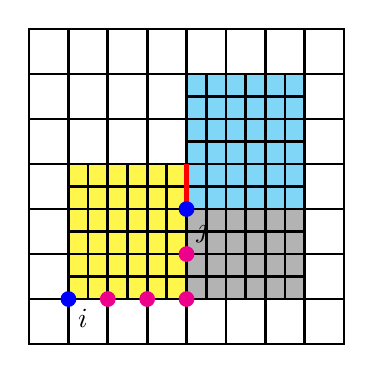
\begin{tikzpicture}[scale=4.0]
    % Define layers
    \pgfdeclarelayer{background}
    \pgfsetlayers{background,main}

    \coordinate (v1_1) at (0.0, 0.0);
    \coordinate (v1_2) at (0.125, 0.0);
    \coordinate (v1_3) at (0.125, 0.14285714285714285);
    \coordinate (v1_4) at (0.0, 0.14285714285714285);
    \draw[black, line width=1.0pt] (v1_1) -- (v1_2) -- (v1_3) -- (v1_4) -- cycle;
    \coordinate (v2_1) at (0.125, 0.0);
    \coordinate (v2_2) at (0.25, 0.0);
    \coordinate (v2_3) at (0.25, 0.14285714285714285);
    \coordinate (v2_4) at (0.125, 0.14285714285714285);
    \draw[black, line width=1.0pt] (v2_1) -- (v2_2) -- (v2_3) -- (v2_4) -- cycle;
    \coordinate (v3_1) at (0.25, 0.0);
    \coordinate (v3_2) at (0.375, 0.0);
    \coordinate (v3_3) at (0.375, 0.14285714285714285);
    \coordinate (v3_4) at (0.25, 0.14285714285714285);
    \draw[black, line width=1.0pt] (v3_1) -- (v3_2) -- (v3_3) -- (v3_4) -- cycle;
    \coordinate (v4_1) at (0.375, 0.0);
    \coordinate (v4_2) at (0.5, 0.0);
    \coordinate (v4_3) at (0.5, 0.14285714285714285);
    \coordinate (v4_4) at (0.375, 0.14285714285714285);
    \draw[black, line width=1.0pt] (v4_1) -- (v4_2) -- (v4_3) -- (v4_4) -- cycle;
    \coordinate (v5_1) at (0.5, 0.0);
    \coordinate (v5_2) at (0.625, 0.0);
    \coordinate (v5_3) at (0.625, 0.14285714285714285);
    \coordinate (v5_4) at (0.5, 0.14285714285714285);
    \draw[black, line width=1.0pt] (v5_1) -- (v5_2) -- (v5_3) -- (v5_4) -- cycle;
    \coordinate (v6_1) at (0.625, 0.0);
    \coordinate (v6_2) at (0.75, 0.0);
    \coordinate (v6_3) at (0.75, 0.14285714285714285);
    \coordinate (v6_4) at (0.625, 0.14285714285714285);
    \draw[black, line width=1.0pt] (v6_1) -- (v6_2) -- (v6_3) -- (v6_4) -- cycle;
    \coordinate (v7_1) at (0.75, 0.0);
    \coordinate (v7_2) at (0.875, 0.0);
    \coordinate (v7_3) at (0.875, 0.14285714285714285);
    \coordinate (v7_4) at (0.75, 0.14285714285714285);
    \draw[black, line width=1.0pt] (v7_1) -- (v7_2) -- (v7_3) -- (v7_4) -- cycle;
    \coordinate (v8_1) at (0.875, 0.0);
    \coordinate (v8_2) at (1.0, 0.0);
    \coordinate (v8_3) at (1.0, 0.14285714285714285);
    \coordinate (v8_4) at (0.875, 0.14285714285714285);
    \draw[black, line width=1.0pt] (v8_1) -- (v8_2) -- (v8_3) -- (v8_4) -- cycle;
    \coordinate (v9_1) at (0.0, 0.14285714285714285);
    \coordinate (v9_2) at (0.125, 0.14285714285714285);
    \coordinate (v9_3) at (0.125, 0.2857142857142857);
    \coordinate (v9_4) at (0.0, 0.2857142857142857);
    \draw[black, line width=1.0pt] (v9_1) -- (v9_2) -- (v9_3) -- (v9_4) -- cycle;
    \coordinate (v10_1) at (0.875, 0.14285714285714285);
    \coordinate (v10_2) at (1.0, 0.14285714285714285);
    \coordinate (v10_3) at (1.0, 0.2857142857142857);
    \coordinate (v10_4) at (0.875, 0.2857142857142857);
    \draw[black, line width=1.0pt] (v10_1) -- (v10_2) -- (v10_3) -- (v10_4) -- cycle;
    \coordinate (v11_1) at (0.0, 0.2857142857142857);
    \coordinate (v11_2) at (0.125, 0.2857142857142857);
    \coordinate (v11_3) at (0.125, 0.42857142857142855);
    \coordinate (v11_4) at (0.0, 0.42857142857142855);
    \draw[black, line width=1.0pt] (v11_1) -- (v11_2) -- (v11_3) -- (v11_4) -- cycle;
    \coordinate (v12_1) at (0.875, 0.2857142857142857);
    \coordinate (v12_2) at (1.0, 0.2857142857142857);
    \coordinate (v12_3) at (1.0, 0.42857142857142855);
    \coordinate (v12_4) at (0.875, 0.42857142857142855);
    \draw[black, line width=1.0pt] (v12_1) -- (v12_2) -- (v12_3) -- (v12_4) -- cycle;
    \coordinate (v13_1) at (0.0, 0.42857142857142855);
    \coordinate (v13_2) at (0.125, 0.42857142857142855);
    \coordinate (v13_3) at (0.125, 0.5714285714285714);
    \coordinate (v13_4) at (0.0, 0.5714285714285714);
    \draw[black, line width=1.0pt] (v13_1) -- (v13_2) -- (v13_3) -- (v13_4) -- cycle;
    \coordinate (v14_1) at (0.875, 0.42857142857142855);
    \coordinate (v14_2) at (1.0, 0.42857142857142855);
    \coordinate (v14_3) at (1.0, 0.5714285714285714);
    \coordinate (v14_4) at (0.875, 0.5714285714285714);
    \draw[black, line width=1.0pt] (v14_1) -- (v14_2) -- (v14_3) -- (v14_4) -- cycle;
    \coordinate (v15_1) at (0.0, 0.5714285714285714);
    \coordinate (v15_2) at (0.125, 0.5714285714285714);
    \coordinate (v15_3) at (0.125, 0.7142857142857143);
    \coordinate (v15_4) at (0.0, 0.7142857142857143);
    \draw[black, line width=1.0pt] (v15_1) -- (v15_2) -- (v15_3) -- (v15_4) -- cycle;
    \coordinate (v16_1) at (0.125, 0.5714285714285714);
    \coordinate (v16_2) at (0.25, 0.5714285714285714);
    \coordinate (v16_3) at (0.25, 0.7142857142857143);
    \coordinate (v16_4) at (0.125, 0.7142857142857143);
    \draw[black, line width=1.0pt] (v16_1) -- (v16_2) -- (v16_3) -- (v16_4) -- cycle;
    \coordinate (v17_1) at (0.25, 0.5714285714285714);
    \coordinate (v17_2) at (0.375, 0.5714285714285714);
    \coordinate (v17_3) at (0.375, 0.7142857142857143);
    \coordinate (v17_4) at (0.25, 0.7142857142857143);
    \draw[black, line width=1.0pt] (v17_1) -- (v17_2) -- (v17_3) -- (v17_4) -- cycle;
    \coordinate (v18_1) at (0.375, 0.5714285714285714);
    \coordinate (v18_2) at (0.5, 0.5714285714285714);
    \coordinate (v18_3) at (0.5, 0.7142857142857143);
    \coordinate (v18_4) at (0.375, 0.7142857142857143);
    \draw[black, line width=1.0pt] (v18_1) -- (v18_2) -- (v18_3) -- (v18_4) -- cycle;
    \coordinate (v19_1) at (0.875, 0.5714285714285714);
    \coordinate (v19_2) at (1.0, 0.5714285714285714);
    \coordinate (v19_3) at (1.0, 0.7142857142857143);
    \coordinate (v19_4) at (0.875, 0.7142857142857143);
    \draw[black, line width=1.0pt] (v19_1) -- (v19_2) -- (v19_3) -- (v19_4) -- cycle;
    \coordinate (v20_1) at (0.0, 0.7142857142857143);
    \coordinate (v20_2) at (0.125, 0.7142857142857143);
    \coordinate (v20_3) at (0.125, 0.8571428571428571);
    \coordinate (v20_4) at (0.0, 0.8571428571428571);
    \draw[black, line width=1.0pt] (v20_1) -- (v20_2) -- (v20_3) -- (v20_4) -- cycle;
    \coordinate (v21_1) at (0.125, 0.7142857142857143);
    \coordinate (v21_2) at (0.25, 0.7142857142857143);
    \coordinate (v21_3) at (0.25, 0.8571428571428571);
    \coordinate (v21_4) at (0.125, 0.8571428571428571);
    \draw[black, line width=1.0pt] (v21_1) -- (v21_2) -- (v21_3) -- (v21_4) -- cycle;
    \coordinate (v22_1) at (0.25, 0.7142857142857143);
    \coordinate (v22_2) at (0.375, 0.7142857142857143);
    \coordinate (v22_3) at (0.375, 0.8571428571428571);
    \coordinate (v22_4) at (0.25, 0.8571428571428571);
    \draw[black, line width=1.0pt] (v22_1) -- (v22_2) -- (v22_3) -- (v22_4) -- cycle;
    \coordinate (v23_1) at (0.375, 0.7142857142857143);
    \coordinate (v23_2) at (0.5, 0.7142857142857143);
    \coordinate (v23_3) at (0.5, 0.8571428571428571);
    \coordinate (v23_4) at (0.375, 0.8571428571428571);
    \draw[black, line width=1.0pt] (v23_1) -- (v23_2) -- (v23_3) -- (v23_4) -- cycle;
    \coordinate (v24_1) at (0.875, 0.7142857142857143);
    \coordinate (v24_2) at (1.0, 0.7142857142857143);
    \coordinate (v24_3) at (1.0, 0.8571428571428571);
    \coordinate (v24_4) at (0.875, 0.8571428571428571);
    \draw[black, line width=1.0pt] (v24_1) -- (v24_2) -- (v24_3) -- (v24_4) -- cycle;
    \coordinate (v25_1) at (0.0, 0.8571428571428571);
    \coordinate (v25_2) at (0.125, 0.8571428571428571);
    \coordinate (v25_3) at (0.125, 1.0);
    \coordinate (v25_4) at (0.0, 1.0);
    \draw[black, line width=1.0pt] (v25_1) -- (v25_2) -- (v25_3) -- (v25_4) -- cycle;
    \coordinate (v26_1) at (0.125, 0.8571428571428571);
    \coordinate (v26_2) at (0.25, 0.8571428571428571);
    \coordinate (v26_3) at (0.25, 1.0);
    \coordinate (v26_4) at (0.125, 1.0);
    \draw[black, line width=1.0pt] (v26_1) -- (v26_2) -- (v26_3) -- (v26_4) -- cycle;
    \coordinate (v27_1) at (0.25, 0.8571428571428571);
    \coordinate (v27_2) at (0.375, 0.8571428571428571);
    \coordinate (v27_3) at (0.375, 1.0);
    \coordinate (v27_4) at (0.25, 1.0);
    \draw[black, line width=1.0pt] (v27_1) -- (v27_2) -- (v27_3) -- (v27_4) -- cycle;
    \coordinate (v28_1) at (0.375, 0.8571428571428571);
    \coordinate (v28_2) at (0.5, 0.8571428571428571);
    \coordinate (v28_3) at (0.5, 1.0);
    \coordinate (v28_4) at (0.375, 1.0);
    \draw[black, line width=1.0pt] (v28_1) -- (v28_2) -- (v28_3) -- (v28_4) -- cycle;
    \coordinate (v29_1) at (0.5, 0.8571428571428571);
    \coordinate (v29_2) at (0.625, 0.8571428571428571);
    \coordinate (v29_3) at (0.625, 1.0);
    \coordinate (v29_4) at (0.5, 1.0);
    \draw[black, line width=1.0pt] (v29_1) -- (v29_2) -- (v29_3) -- (v29_4) -- cycle;
    \coordinate (v30_1) at (0.625, 0.8571428571428571);
    \coordinate (v30_2) at (0.75, 0.8571428571428571);
    \coordinate (v30_3) at (0.75, 1.0);
    \coordinate (v30_4) at (0.625, 1.0);
    \draw[black, line width=1.0pt] (v30_1) -- (v30_2) -- (v30_3) -- (v30_4) -- cycle;
    \coordinate (v31_1) at (0.75, 0.8571428571428571);
    \coordinate (v31_2) at (0.875, 0.8571428571428571);
    \coordinate (v31_3) at (0.875, 1.0);
    \coordinate (v31_4) at (0.75, 1.0);
    \draw[black, line width=1.0pt] (v31_1) -- (v31_2) -- (v31_3) -- (v31_4) -- cycle;
    \coordinate (v32_1) at (0.875, 0.8571428571428571);
    \coordinate (v32_2) at (1.0, 0.8571428571428571);
    \coordinate (v32_3) at (1.0, 1.0);
    \coordinate (v32_4) at (0.875, 1.0);
    \draw[black, line width=1.0pt] (v32_1) -- (v32_2) -- (v32_3) -- (v32_4) -- cycle;
    \coordinate (v33_1) at (0.125, 0.14285714285714285);
    \coordinate (v33_2) at (0.1875, 0.14285714285714285);
    \coordinate (v33_3) at (0.1875, 0.21428571428571427);
    \coordinate (v33_4) at (0.125, 0.21428571428571427);
    \draw[black, line width=1.0pt] (v33_1) -- (v33_2) -- (v33_3) -- (v33_4) -- cycle;
    \coordinate (v34_1) at (0.1875, 0.14285714285714285);
    \coordinate (v34_2) at (0.25, 0.14285714285714285);
    \coordinate (v34_3) at (0.25, 0.21428571428571427);
    \coordinate (v34_4) at (0.1875, 0.21428571428571427);
    \draw[black, line width=1.0pt] (v34_1) -- (v34_2) -- (v34_3) -- (v34_4) -- cycle;
    \coordinate (v35_1) at (0.25, 0.14285714285714285);
    \coordinate (v35_2) at (0.3125, 0.14285714285714285);
    \coordinate (v35_3) at (0.3125, 0.21428571428571427);
    \coordinate (v35_4) at (0.25, 0.21428571428571427);
    \draw[black, line width=1.0pt] (v35_1) -- (v35_2) -- (v35_3) -- (v35_4) -- cycle;
    \coordinate (v36_1) at (0.3125, 0.14285714285714285);
    \coordinate (v36_2) at (0.375, 0.14285714285714285);
    \coordinate (v36_3) at (0.375, 0.21428571428571427);
    \coordinate (v36_4) at (0.3125, 0.21428571428571427);
    \draw[black, line width=1.0pt] (v36_1) -- (v36_2) -- (v36_3) -- (v36_4) -- cycle;
    \coordinate (v37_1) at (0.375, 0.14285714285714285);
    \coordinate (v37_2) at (0.4375, 0.14285714285714285);
    \coordinate (v37_3) at (0.4375, 0.21428571428571427);
    \coordinate (v37_4) at (0.375, 0.21428571428571427);
    \draw[black, line width=1.0pt] (v37_1) -- (v37_2) -- (v37_3) -- (v37_4) -- cycle;
    \coordinate (v38_1) at (0.4375, 0.14285714285714285);
    \coordinate (v38_2) at (0.5, 0.14285714285714285);
    \coordinate (v38_3) at (0.5, 0.21428571428571427);
    \coordinate (v38_4) at (0.4375, 0.21428571428571427);
    \draw[black, line width=1.0pt] (v38_1) -- (v38_2) -- (v38_3) -- (v38_4) -- cycle;
    \coordinate (v39_1) at (0.5, 0.14285714285714285);
    \coordinate (v39_2) at (0.5625, 0.14285714285714285);
    \coordinate (v39_3) at (0.5625, 0.21428571428571427);
    \coordinate (v39_4) at (0.5, 0.21428571428571427);
    \draw[black, line width=1.0pt] (v39_1) -- (v39_2) -- (v39_3) -- (v39_4) -- cycle;
    \coordinate (v40_1) at (0.5625, 0.14285714285714285);
    \coordinate (v40_2) at (0.625, 0.14285714285714285);
    \coordinate (v40_3) at (0.625, 0.21428571428571427);
    \coordinate (v40_4) at (0.5625, 0.21428571428571427);
    \draw[black, line width=1.0pt] (v40_1) -- (v40_2) -- (v40_3) -- (v40_4) -- cycle;
    \coordinate (v41_1) at (0.625, 0.14285714285714285);
    \coordinate (v41_2) at (0.6875, 0.14285714285714285);
    \coordinate (v41_3) at (0.6875, 0.21428571428571427);
    \coordinate (v41_4) at (0.625, 0.21428571428571427);
    \draw[black, line width=1.0pt] (v41_1) -- (v41_2) -- (v41_3) -- (v41_4) -- cycle;
    \coordinate (v42_1) at (0.6875, 0.14285714285714285);
    \coordinate (v42_2) at (0.75, 0.14285714285714285);
    \coordinate (v42_3) at (0.75, 0.21428571428571427);
    \coordinate (v42_4) at (0.6875, 0.21428571428571427);
    \draw[black, line width=1.0pt] (v42_1) -- (v42_2) -- (v42_3) -- (v42_4) -- cycle;
    \coordinate (v43_1) at (0.75, 0.14285714285714285);
    \coordinate (v43_2) at (0.8125, 0.14285714285714285);
    \coordinate (v43_3) at (0.8125, 0.21428571428571427);
    \coordinate (v43_4) at (0.75, 0.21428571428571427);
    \draw[black, line width=1.0pt] (v43_1) -- (v43_2) -- (v43_3) -- (v43_4) -- cycle;
    \coordinate (v44_1) at (0.8125, 0.14285714285714285);
    \coordinate (v44_2) at (0.875, 0.14285714285714285);
    \coordinate (v44_3) at (0.875, 0.21428571428571427);
    \coordinate (v44_4) at (0.8125, 0.21428571428571427);
    \draw[black, line width=1.0pt] (v44_1) -- (v44_2) -- (v44_3) -- (v44_4) -- cycle;
    \coordinate (v45_1) at (0.125, 0.21428571428571427);
    \coordinate (v45_2) at (0.1875, 0.21428571428571427);
    \coordinate (v45_3) at (0.1875, 0.2857142857142857);
    \coordinate (v45_4) at (0.125, 0.2857142857142857);
    \draw[black, line width=1.0pt] (v45_1) -- (v45_2) -- (v45_3) -- (v45_4) -- cycle;
    \coordinate (v46_1) at (0.1875, 0.21428571428571427);
    \coordinate (v46_2) at (0.25, 0.21428571428571427);
    \coordinate (v46_3) at (0.25, 0.2857142857142857);
    \coordinate (v46_4) at (0.1875, 0.2857142857142857);
    \draw[black, line width=1.0pt] (v46_1) -- (v46_2) -- (v46_3) -- (v46_4) -- cycle;
    \coordinate (v47_1) at (0.25, 0.21428571428571427);
    \coordinate (v47_2) at (0.3125, 0.21428571428571427);
    \coordinate (v47_3) at (0.3125, 0.2857142857142857);
    \coordinate (v47_4) at (0.25, 0.2857142857142857);
    \draw[black, line width=1.0pt] (v47_1) -- (v47_2) -- (v47_3) -- (v47_4) -- cycle;
    \coordinate (v48_1) at (0.3125, 0.21428571428571427);
    \coordinate (v48_2) at (0.375, 0.21428571428571427);
    \coordinate (v48_3) at (0.375, 0.2857142857142857);
    \coordinate (v48_4) at (0.3125, 0.2857142857142857);
    \draw[black, line width=1.0pt] (v48_1) -- (v48_2) -- (v48_3) -- (v48_4) -- cycle;
    \coordinate (v49_1) at (0.375, 0.21428571428571427);
    \coordinate (v49_2) at (0.4375, 0.21428571428571427);
    \coordinate (v49_3) at (0.4375, 0.2857142857142857);
    \coordinate (v49_4) at (0.375, 0.2857142857142857);
    \draw[black, line width=1.0pt] (v49_1) -- (v49_2) -- (v49_3) -- (v49_4) -- cycle;
    \coordinate (v50_1) at (0.4375, 0.21428571428571427);
    \coordinate (v50_2) at (0.5, 0.21428571428571427);
    \coordinate (v50_3) at (0.5, 0.2857142857142857);
    \coordinate (v50_4) at (0.4375, 0.2857142857142857);
    \draw[black, line width=1.0pt] (v50_1) -- (v50_2) -- (v50_3) -- (v50_4) -- cycle;
    \coordinate (v51_1) at (0.5, 0.21428571428571427);
    \coordinate (v51_2) at (0.5625, 0.21428571428571427);
    \coordinate (v51_3) at (0.5625, 0.2857142857142857);
    \coordinate (v51_4) at (0.5, 0.2857142857142857);
    \draw[black, line width=1.0pt] (v51_1) -- (v51_2) -- (v51_3) -- (v51_4) -- cycle;
    \coordinate (v52_1) at (0.5625, 0.21428571428571427);
    \coordinate (v52_2) at (0.625, 0.21428571428571427);
    \coordinate (v52_3) at (0.625, 0.2857142857142857);
    \coordinate (v52_4) at (0.5625, 0.2857142857142857);
    \draw[black, line width=1.0pt] (v52_1) -- (v52_2) -- (v52_3) -- (v52_4) -- cycle;
    \coordinate (v53_1) at (0.625, 0.21428571428571427);
    \coordinate (v53_2) at (0.6875, 0.21428571428571427);
    \coordinate (v53_3) at (0.6875, 0.2857142857142857);
    \coordinate (v53_4) at (0.625, 0.2857142857142857);
    \draw[black, line width=1.0pt] (v53_1) -- (v53_2) -- (v53_3) -- (v53_4) -- cycle;
    \coordinate (v54_1) at (0.6875, 0.21428571428571427);
    \coordinate (v54_2) at (0.75, 0.21428571428571427);
    \coordinate (v54_3) at (0.75, 0.2857142857142857);
    \coordinate (v54_4) at (0.6875, 0.2857142857142857);
    \draw[black, line width=1.0pt] (v54_1) -- (v54_2) -- (v54_3) -- (v54_4) -- cycle;
    \coordinate (v55_1) at (0.75, 0.21428571428571427);
    \coordinate (v55_2) at (0.8125, 0.21428571428571427);
    \coordinate (v55_3) at (0.8125, 0.2857142857142857);
    \coordinate (v55_4) at (0.75, 0.2857142857142857);
    \draw[black, line width=1.0pt] (v55_1) -- (v55_2) -- (v55_3) -- (v55_4) -- cycle;
    \coordinate (v56_1) at (0.8125, 0.21428571428571427);
    \coordinate (v56_2) at (0.875, 0.21428571428571427);
    \coordinate (v56_3) at (0.875, 0.2857142857142857);
    \coordinate (v56_4) at (0.8125, 0.2857142857142857);
    \draw[black, line width=1.0pt] (v56_1) -- (v56_2) -- (v56_3) -- (v56_4) -- cycle;
    \coordinate (v57_1) at (0.125, 0.2857142857142857);
    \coordinate (v57_2) at (0.1875, 0.2857142857142857);
    \coordinate (v57_3) at (0.1875, 0.3571428571428571);
    \coordinate (v57_4) at (0.125, 0.3571428571428571);
    \draw[black, line width=1.0pt] (v57_1) -- (v57_2) -- (v57_3) -- (v57_4) -- cycle;
    \coordinate (v58_1) at (0.1875, 0.2857142857142857);
    \coordinate (v58_2) at (0.25, 0.2857142857142857);
    \coordinate (v58_3) at (0.25, 0.3571428571428571);
    \coordinate (v58_4) at (0.1875, 0.3571428571428571);
    \draw[black, line width=1.0pt] (v58_1) -- (v58_2) -- (v58_3) -- (v58_4) -- cycle;
    \coordinate (v59_1) at (0.25, 0.2857142857142857);
    \coordinate (v59_2) at (0.3125, 0.2857142857142857);
    \coordinate (v59_3) at (0.3125, 0.3571428571428571);
    \coordinate (v59_4) at (0.25, 0.3571428571428571);
    \draw[black, line width=1.0pt] (v59_1) -- (v59_2) -- (v59_3) -- (v59_4) -- cycle;
    \coordinate (v60_1) at (0.3125, 0.2857142857142857);
    \coordinate (v60_2) at (0.375, 0.2857142857142857);
    \coordinate (v60_3) at (0.375, 0.3571428571428571);
    \coordinate (v60_4) at (0.3125, 0.3571428571428571);
    \draw[black, line width=1.0pt] (v60_1) -- (v60_2) -- (v60_3) -- (v60_4) -- cycle;
    \coordinate (v61_1) at (0.375, 0.2857142857142857);
    \coordinate (v61_2) at (0.4375, 0.2857142857142857);
    \coordinate (v61_3) at (0.4375, 0.3571428571428571);
    \coordinate (v61_4) at (0.375, 0.3571428571428571);
    \draw[black, line width=1.0pt] (v61_1) -- (v61_2) -- (v61_3) -- (v61_4) -- cycle;
    \coordinate (v62_1) at (0.4375, 0.2857142857142857);
    \coordinate (v62_2) at (0.5, 0.2857142857142857);
    \coordinate (v62_3) at (0.5, 0.3571428571428571);
    \coordinate (v62_4) at (0.4375, 0.3571428571428571);
    \draw[black, line width=1.0pt] (v62_1) -- (v62_2) -- (v62_3) -- (v62_4) -- cycle;
    \coordinate (v63_1) at (0.5, 0.2857142857142857);
    \coordinate (v63_2) at (0.5625, 0.2857142857142857);
    \coordinate (v63_3) at (0.5625, 0.3571428571428571);
    \coordinate (v63_4) at (0.5, 0.3571428571428571);
    \draw[black, line width=1.0pt] (v63_1) -- (v63_2) -- (v63_3) -- (v63_4) -- cycle;
    \coordinate (v64_1) at (0.5625, 0.2857142857142857);
    \coordinate (v64_2) at (0.625, 0.2857142857142857);
    \coordinate (v64_3) at (0.625, 0.3571428571428571);
    \coordinate (v64_4) at (0.5625, 0.3571428571428571);
    \draw[black, line width=1.0pt] (v64_1) -- (v64_2) -- (v64_3) -- (v64_4) -- cycle;
    \coordinate (v65_1) at (0.625, 0.2857142857142857);
    \coordinate (v65_2) at (0.6875, 0.2857142857142857);
    \coordinate (v65_3) at (0.6875, 0.3571428571428571);
    \coordinate (v65_4) at (0.625, 0.3571428571428571);
    \draw[black, line width=1.0pt] (v65_1) -- (v65_2) -- (v65_3) -- (v65_4) -- cycle;
    \coordinate (v66_1) at (0.6875, 0.2857142857142857);
    \coordinate (v66_2) at (0.75, 0.2857142857142857);
    \coordinate (v66_3) at (0.75, 0.3571428571428571);
    \coordinate (v66_4) at (0.6875, 0.3571428571428571);
    \draw[black, line width=1.0pt] (v66_1) -- (v66_2) -- (v66_3) -- (v66_4) -- cycle;
    \coordinate (v67_1) at (0.75, 0.2857142857142857);
    \coordinate (v67_2) at (0.8125, 0.2857142857142857);
    \coordinate (v67_3) at (0.8125, 0.3571428571428571);
    \coordinate (v67_4) at (0.75, 0.3571428571428571);
    \draw[black, line width=1.0pt] (v67_1) -- (v67_2) -- (v67_3) -- (v67_4) -- cycle;
    \coordinate (v68_1) at (0.8125, 0.2857142857142857);
    \coordinate (v68_2) at (0.875, 0.2857142857142857);
    \coordinate (v68_3) at (0.875, 0.3571428571428571);
    \coordinate (v68_4) at (0.8125, 0.3571428571428571);
    \draw[black, line width=1.0pt] (v68_1) -- (v68_2) -- (v68_3) -- (v68_4) -- cycle;
    \coordinate (v69_1) at (0.125, 0.3571428571428571);
    \coordinate (v69_2) at (0.1875, 0.3571428571428571);
    \coordinate (v69_3) at (0.1875, 0.42857142857142855);
    \coordinate (v69_4) at (0.125, 0.42857142857142855);
    \draw[black, line width=1.0pt] (v69_1) -- (v69_2) -- (v69_3) -- (v69_4) -- cycle;
    \coordinate (v70_1) at (0.1875, 0.3571428571428571);
    \coordinate (v70_2) at (0.25, 0.3571428571428571);
    \coordinate (v70_3) at (0.25, 0.42857142857142855);
    \coordinate (v70_4) at (0.1875, 0.42857142857142855);
    \draw[black, line width=1.0pt] (v70_1) -- (v70_2) -- (v70_3) -- (v70_4) -- cycle;
    \coordinate (v71_1) at (0.25, 0.3571428571428571);
    \coordinate (v71_2) at (0.3125, 0.3571428571428571);
    \coordinate (v71_3) at (0.3125, 0.42857142857142855);
    \coordinate (v71_4) at (0.25, 0.42857142857142855);
    \draw[black, line width=1.0pt] (v71_1) -- (v71_2) -- (v71_3) -- (v71_4) -- cycle;
    \coordinate (v72_1) at (0.3125, 0.3571428571428571);
    \coordinate (v72_2) at (0.375, 0.3571428571428571);
    \coordinate (v72_3) at (0.375, 0.42857142857142855);
    \coordinate (v72_4) at (0.3125, 0.42857142857142855);
    \draw[black, line width=1.0pt] (v72_1) -- (v72_2) -- (v72_3) -- (v72_4) -- cycle;
    \coordinate (v73_1) at (0.375, 0.3571428571428571);
    \coordinate (v73_2) at (0.4375, 0.3571428571428571);
    \coordinate (v73_3) at (0.4375, 0.42857142857142855);
    \coordinate (v73_4) at (0.375, 0.42857142857142855);
    \draw[black, line width=1.0pt] (v73_1) -- (v73_2) -- (v73_3) -- (v73_4) -- cycle;
    \coordinate (v74_1) at (0.4375, 0.3571428571428571);
    \coordinate (v74_2) at (0.5, 0.3571428571428571);
    \coordinate (v74_3) at (0.5, 0.42857142857142855);
    \coordinate (v74_4) at (0.4375, 0.42857142857142855);
    \draw[black, line width=1.0pt] (v74_1) -- (v74_2) -- (v74_3) -- (v74_4) -- cycle;
    \coordinate (v75_1) at (0.5, 0.3571428571428571);
    \coordinate (v75_2) at (0.5625, 0.3571428571428571);
    \coordinate (v75_3) at (0.5625, 0.42857142857142855);
    \coordinate (v75_4) at (0.5, 0.42857142857142855);
    \draw[black, line width=1.0pt] (v75_1) -- (v75_2) -- (v75_3) -- (v75_4) -- cycle;
    \coordinate (v76_1) at (0.5625, 0.3571428571428571);
    \coordinate (v76_2) at (0.625, 0.3571428571428571);
    \coordinate (v76_3) at (0.625, 0.42857142857142855);
    \coordinate (v76_4) at (0.5625, 0.42857142857142855);
    \draw[black, line width=1.0pt] (v76_1) -- (v76_2) -- (v76_3) -- (v76_4) -- cycle;
    \coordinate (v77_1) at (0.625, 0.3571428571428571);
    \coordinate (v77_2) at (0.6875, 0.3571428571428571);
    \coordinate (v77_3) at (0.6875, 0.42857142857142855);
    \coordinate (v77_4) at (0.625, 0.42857142857142855);
    \draw[black, line width=1.0pt] (v77_1) -- (v77_2) -- (v77_3) -- (v77_4) -- cycle;
    \coordinate (v78_1) at (0.6875, 0.3571428571428571);
    \coordinate (v78_2) at (0.75, 0.3571428571428571);
    \coordinate (v78_3) at (0.75, 0.42857142857142855);
    \coordinate (v78_4) at (0.6875, 0.42857142857142855);
    \draw[black, line width=1.0pt] (v78_1) -- (v78_2) -- (v78_3) -- (v78_4) -- cycle;
    \coordinate (v79_1) at (0.75, 0.3571428571428571);
    \coordinate (v79_2) at (0.8125, 0.3571428571428571);
    \coordinate (v79_3) at (0.8125, 0.42857142857142855);
    \coordinate (v79_4) at (0.75, 0.42857142857142855);
    \draw[black, line width=1.0pt] (v79_1) -- (v79_2) -- (v79_3) -- (v79_4) -- cycle;
    \coordinate (v80_1) at (0.8125, 0.3571428571428571);
    \coordinate (v80_2) at (0.875, 0.3571428571428571);
    \coordinate (v80_3) at (0.875, 0.42857142857142855);
    \coordinate (v80_4) at (0.8125, 0.42857142857142855);
    \draw[black, line width=1.0pt] (v80_1) -- (v80_2) -- (v80_3) -- (v80_4) -- cycle;
    \coordinate (v81_1) at (0.125, 0.42857142857142855);
    \coordinate (v81_2) at (0.1875, 0.42857142857142855);
    \coordinate (v81_3) at (0.1875, 0.5);
    \coordinate (v81_4) at (0.125, 0.5);
    \draw[black, line width=1.0pt] (v81_1) -- (v81_2) -- (v81_3) -- (v81_4) -- cycle;
    \coordinate (v82_1) at (0.1875, 0.42857142857142855);
    \coordinate (v82_2) at (0.25, 0.42857142857142855);
    \coordinate (v82_3) at (0.25, 0.5);
    \coordinate (v82_4) at (0.1875, 0.5);
    \draw[black, line width=1.0pt] (v82_1) -- (v82_2) -- (v82_3) -- (v82_4) -- cycle;
    \coordinate (v83_1) at (0.25, 0.42857142857142855);
    \coordinate (v83_2) at (0.3125, 0.42857142857142855);
    \coordinate (v83_3) at (0.3125, 0.5);
    \coordinate (v83_4) at (0.25, 0.5);
    \draw[black, line width=1.0pt] (v83_1) -- (v83_2) -- (v83_3) -- (v83_4) -- cycle;
    \coordinate (v84_1) at (0.3125, 0.42857142857142855);
    \coordinate (v84_2) at (0.375, 0.42857142857142855);
    \coordinate (v84_3) at (0.375, 0.5);
    \coordinate (v84_4) at (0.3125, 0.5);
    \draw[black, line width=1.0pt] (v84_1) -- (v84_2) -- (v84_3) -- (v84_4) -- cycle;
    \coordinate (v85_1) at (0.375, 0.42857142857142855);
    \coordinate (v85_2) at (0.4375, 0.42857142857142855);
    \coordinate (v85_3) at (0.4375, 0.5);
    \coordinate (v85_4) at (0.375, 0.5);
    \draw[black, line width=1.0pt] (v85_1) -- (v85_2) -- (v85_3) -- (v85_4) -- cycle;
    \coordinate (v86_1) at (0.4375, 0.42857142857142855);
    \coordinate (v86_2) at (0.5, 0.42857142857142855);
    \coordinate (v86_3) at (0.5, 0.5);
    \coordinate (v86_4) at (0.4375, 0.5);
    \draw[black, line width=1.0pt] (v86_1) -- (v86_2) -- (v86_3) -- (v86_4) -- cycle;
    \coordinate (v87_1) at (0.5, 0.42857142857142855);
    \coordinate (v87_2) at (0.5625, 0.42857142857142855);
    \coordinate (v87_3) at (0.5625, 0.5);
    \coordinate (v87_4) at (0.5, 0.5);
    \draw[black, line width=1.0pt] (v87_1) -- (v87_2) -- (v87_3) -- (v87_4) -- cycle;
    \coordinate (v88_1) at (0.5625, 0.42857142857142855);
    \coordinate (v88_2) at (0.625, 0.42857142857142855);
    \coordinate (v88_3) at (0.625, 0.5);
    \coordinate (v88_4) at (0.5625, 0.5);
    \draw[black, line width=1.0pt] (v88_1) -- (v88_2) -- (v88_3) -- (v88_4) -- cycle;
    \coordinate (v89_1) at (0.625, 0.42857142857142855);
    \coordinate (v89_2) at (0.6875, 0.42857142857142855);
    \coordinate (v89_3) at (0.6875, 0.5);
    \coordinate (v89_4) at (0.625, 0.5);
    \draw[black, line width=1.0pt] (v89_1) -- (v89_2) -- (v89_3) -- (v89_4) -- cycle;
    \coordinate (v90_1) at (0.6875, 0.42857142857142855);
    \coordinate (v90_2) at (0.75, 0.42857142857142855);
    \coordinate (v90_3) at (0.75, 0.5);
    \coordinate (v90_4) at (0.6875, 0.5);
    \draw[black, line width=1.0pt] (v90_1) -- (v90_2) -- (v90_3) -- (v90_4) -- cycle;
    \coordinate (v91_1) at (0.75, 0.42857142857142855);
    \coordinate (v91_2) at (0.8125, 0.42857142857142855);
    \coordinate (v91_3) at (0.8125, 0.5);
    \coordinate (v91_4) at (0.75, 0.5);
    \draw[black, line width=1.0pt] (v91_1) -- (v91_2) -- (v91_3) -- (v91_4) -- cycle;
    \coordinate (v92_1) at (0.8125, 0.42857142857142855);
    \coordinate (v92_2) at (0.875, 0.42857142857142855);
    \coordinate (v92_3) at (0.875, 0.5);
    \coordinate (v92_4) at (0.8125, 0.5);
    \draw[black, line width=1.0pt] (v92_1) -- (v92_2) -- (v92_3) -- (v92_4) -- cycle;
    \coordinate (v93_1) at (0.125, 0.5);
    \coordinate (v93_2) at (0.1875, 0.5);
    \coordinate (v93_3) at (0.1875, 0.5714285714285714);
    \coordinate (v93_4) at (0.125, 0.5714285714285714);
    \draw[black, line width=1.0pt] (v93_1) -- (v93_2) -- (v93_3) -- (v93_4) -- cycle;
    \coordinate (v94_1) at (0.1875, 0.5);
    \coordinate (v94_2) at (0.25, 0.5);
    \coordinate (v94_3) at (0.25, 0.5714285714285714);
    \coordinate (v94_4) at (0.1875, 0.5714285714285714);
    \draw[black, line width=1.0pt] (v94_1) -- (v94_2) -- (v94_3) -- (v94_4) -- cycle;
    \coordinate (v95_1) at (0.25, 0.5);
    \coordinate (v95_2) at (0.3125, 0.5);
    \coordinate (v95_3) at (0.3125, 0.5714285714285714);
    \coordinate (v95_4) at (0.25, 0.5714285714285714);
    \draw[black, line width=1.0pt] (v95_1) -- (v95_2) -- (v95_3) -- (v95_4) -- cycle;
    \coordinate (v96_1) at (0.3125, 0.5);
    \coordinate (v96_2) at (0.375, 0.5);
    \coordinate (v96_3) at (0.375, 0.5714285714285714);
    \coordinate (v96_4) at (0.3125, 0.5714285714285714);
    \draw[black, line width=1.0pt] (v96_1) -- (v96_2) -- (v96_3) -- (v96_4) -- cycle;
    \coordinate (v97_1) at (0.375, 0.5);
    \coordinate (v97_2) at (0.4375, 0.5);
    \coordinate (v97_3) at (0.4375, 0.5714285714285714);
    \coordinate (v97_4) at (0.375, 0.5714285714285714);
    \draw[black, line width=1.0pt] (v97_1) -- (v97_2) -- (v97_3) -- (v97_4) -- cycle;
    \coordinate (v98_1) at (0.4375, 0.5);
    \coordinate (v98_2) at (0.5, 0.5);
    \coordinate (v98_3) at (0.5, 0.5714285714285714);
    \coordinate (v98_4) at (0.4375, 0.5714285714285714);
    \draw[black, line width=1.0pt] (v98_1) -- (v98_2) -- (v98_3) -- (v98_4) -- cycle;
    \coordinate (v99_1) at (0.5, 0.5);
    \coordinate (v99_2) at (0.5625, 0.5);
    \coordinate (v99_3) at (0.5625, 0.5714285714285714);
    \coordinate (v99_4) at (0.5, 0.5714285714285714);
    \draw[black, line width=1.0pt] (v99_1) -- (v99_2) -- (v99_3) -- (v99_4) -- cycle;
    \coordinate (v100_1) at (0.5625, 0.5);
    \coordinate (v100_2) at (0.625, 0.5);
    \coordinate (v100_3) at (0.625, 0.5714285714285714);
    \coordinate (v100_4) at (0.5625, 0.5714285714285714);
    \draw[black, line width=1.0pt] (v100_1) -- (v100_2) -- (v100_3) -- (v100_4) -- cycle;
    \coordinate (v101_1) at (0.625, 0.5);
    \coordinate (v101_2) at (0.6875, 0.5);
    \coordinate (v101_3) at (0.6875, 0.5714285714285714);
    \coordinate (v101_4) at (0.625, 0.5714285714285714);
    \draw[black, line width=1.0pt] (v101_1) -- (v101_2) -- (v101_3) -- (v101_4) -- cycle;
    \coordinate (v102_1) at (0.6875, 0.5);
    \coordinate (v102_2) at (0.75, 0.5);
    \coordinate (v102_3) at (0.75, 0.5714285714285714);
    \coordinate (v102_4) at (0.6875, 0.5714285714285714);
    \draw[black, line width=1.0pt] (v102_1) -- (v102_2) -- (v102_3) -- (v102_4) -- cycle;
    \coordinate (v103_1) at (0.75, 0.5);
    \coordinate (v103_2) at (0.8125, 0.5);
    \coordinate (v103_3) at (0.8125, 0.5714285714285714);
    \coordinate (v103_4) at (0.75, 0.5714285714285714);
    \draw[black, line width=1.0pt] (v103_1) -- (v103_2) -- (v103_3) -- (v103_4) -- cycle;
    \coordinate (v104_1) at (0.8125, 0.5);
    \coordinate (v104_2) at (0.875, 0.5);
    \coordinate (v104_3) at (0.875, 0.5714285714285714);
    \coordinate (v104_4) at (0.8125, 0.5714285714285714);
    \draw[black, line width=1.0pt] (v104_1) -- (v104_2) -- (v104_3) -- (v104_4) -- cycle;
    \coordinate (v105_1) at (0.5, 0.5714285714285714);
    \coordinate (v105_2) at (0.5625, 0.5714285714285714);
    \coordinate (v105_3) at (0.5625, 0.6428571428571428);
    \coordinate (v105_4) at (0.5, 0.6428571428571428);
    \draw[black, line width=1.0pt] (v105_1) -- (v105_2) -- (v105_3) -- (v105_4) -- cycle;
    \coordinate (v106_1) at (0.5625, 0.5714285714285714);
    \coordinate (v106_2) at (0.625, 0.5714285714285714);
    \coordinate (v106_3) at (0.625, 0.6428571428571428);
    \coordinate (v106_4) at (0.5625, 0.6428571428571428);
    \draw[black, line width=1.0pt] (v106_1) -- (v106_2) -- (v106_3) -- (v106_4) -- cycle;
    \coordinate (v107_1) at (0.625, 0.5714285714285714);
    \coordinate (v107_2) at (0.6875, 0.5714285714285714);
    \coordinate (v107_3) at (0.6875, 0.6428571428571428);
    \coordinate (v107_4) at (0.625, 0.6428571428571428);
    \draw[black, line width=1.0pt] (v107_1) -- (v107_2) -- (v107_3) -- (v107_4) -- cycle;
    \coordinate (v108_1) at (0.6875, 0.5714285714285714);
    \coordinate (v108_2) at (0.75, 0.5714285714285714);
    \coordinate (v108_3) at (0.75, 0.6428571428571428);
    \coordinate (v108_4) at (0.6875, 0.6428571428571428);
    \draw[black, line width=1.0pt] (v108_1) -- (v108_2) -- (v108_3) -- (v108_4) -- cycle;
    \coordinate (v109_1) at (0.75, 0.5714285714285714);
    \coordinate (v109_2) at (0.8125, 0.5714285714285714);
    \coordinate (v109_3) at (0.8125, 0.6428571428571428);
    \coordinate (v109_4) at (0.75, 0.6428571428571428);
    \draw[black, line width=1.0pt] (v109_1) -- (v109_2) -- (v109_3) -- (v109_4) -- cycle;
    \coordinate (v110_1) at (0.8125, 0.5714285714285714);
    \coordinate (v110_2) at (0.875, 0.5714285714285714);
    \coordinate (v110_3) at (0.875, 0.6428571428571428);
    \coordinate (v110_4) at (0.8125, 0.6428571428571428);
    \draw[black, line width=1.0pt] (v110_1) -- (v110_2) -- (v110_3) -- (v110_4) -- cycle;
    \coordinate (v111_1) at (0.5, 0.6428571428571428);
    \coordinate (v111_2) at (0.5625, 0.6428571428571428);
    \coordinate (v111_3) at (0.5625, 0.7142857142857143);
    \coordinate (v111_4) at (0.5, 0.7142857142857143);
    \draw[black, line width=1.0pt] (v111_1) -- (v111_2) -- (v111_3) -- (v111_4) -- cycle;
    \coordinate (v112_1) at (0.5625, 0.6428571428571428);
    \coordinate (v112_2) at (0.625, 0.6428571428571428);
    \coordinate (v112_3) at (0.625, 0.7142857142857143);
    \coordinate (v112_4) at (0.5625, 0.7142857142857143);
    \draw[black, line width=1.0pt] (v112_1) -- (v112_2) -- (v112_3) -- (v112_4) -- cycle;
    \coordinate (v113_1) at (0.625, 0.6428571428571428);
    \coordinate (v113_2) at (0.6875, 0.6428571428571428);
    \coordinate (v113_3) at (0.6875, 0.7142857142857143);
    \coordinate (v113_4) at (0.625, 0.7142857142857143);
    \draw[black, line width=1.0pt] (v113_1) -- (v113_2) -- (v113_3) -- (v113_4) -- cycle;
    \coordinate (v114_1) at (0.6875, 0.6428571428571428);
    \coordinate (v114_2) at (0.75, 0.6428571428571428);
    \coordinate (v114_3) at (0.75, 0.7142857142857143);
    \coordinate (v114_4) at (0.6875, 0.7142857142857143);
    \draw[black, line width=1.0pt] (v114_1) -- (v114_2) -- (v114_3) -- (v114_4) -- cycle;
    \coordinate (v115_1) at (0.75, 0.6428571428571428);
    \coordinate (v115_2) at (0.8125, 0.6428571428571428);
    \coordinate (v115_3) at (0.8125, 0.7142857142857143);
    \coordinate (v115_4) at (0.75, 0.7142857142857143);
    \draw[black, line width=1.0pt] (v115_1) -- (v115_2) -- (v115_3) -- (v115_4) -- cycle;
    \coordinate (v116_1) at (0.8125, 0.6428571428571428);
    \coordinate (v116_2) at (0.875, 0.6428571428571428);
    \coordinate (v116_3) at (0.875, 0.7142857142857143);
    \coordinate (v116_4) at (0.8125, 0.7142857142857143);
    \draw[black, line width=1.0pt] (v116_1) -- (v116_2) -- (v116_3) -- (v116_4) -- cycle;
    \coordinate (v117_1) at (0.5, 0.7142857142857143);
    \coordinate (v117_2) at (0.5625, 0.7142857142857143);
    \coordinate (v117_3) at (0.5625, 0.7857142857142857);
    \coordinate (v117_4) at (0.5, 0.7857142857142857);
    \draw[black, line width=1.0pt] (v117_1) -- (v117_2) -- (v117_3) -- (v117_4) -- cycle;
    \coordinate (v118_1) at (0.5625, 0.7142857142857143);
    \coordinate (v118_2) at (0.625, 0.7142857142857143);
    \coordinate (v118_3) at (0.625, 0.7857142857142857);
    \coordinate (v118_4) at (0.5625, 0.7857142857142857);
    \draw[black, line width=1.0pt] (v118_1) -- (v118_2) -- (v118_3) -- (v118_4) -- cycle;
    \coordinate (v119_1) at (0.625, 0.7142857142857143);
    \coordinate (v119_2) at (0.6875, 0.7142857142857143);
    \coordinate (v119_3) at (0.6875, 0.7857142857142857);
    \coordinate (v119_4) at (0.625, 0.7857142857142857);
    \draw[black, line width=1.0pt] (v119_1) -- (v119_2) -- (v119_3) -- (v119_4) -- cycle;
    \coordinate (v120_1) at (0.6875, 0.7142857142857143);
    \coordinate (v120_2) at (0.75, 0.7142857142857143);
    \coordinate (v120_3) at (0.75, 0.7857142857142857);
    \coordinate (v120_4) at (0.6875, 0.7857142857142857);
    \draw[black, line width=1.0pt] (v120_1) -- (v120_2) -- (v120_3) -- (v120_4) -- cycle;
    \coordinate (v121_1) at (0.75, 0.7142857142857143);
    \coordinate (v121_2) at (0.8125, 0.7142857142857143);
    \coordinate (v121_3) at (0.8125, 0.7857142857142857);
    \coordinate (v121_4) at (0.75, 0.7857142857142857);
    \draw[black, line width=1.0pt] (v121_1) -- (v121_2) -- (v121_3) -- (v121_4) -- cycle;
    \coordinate (v122_1) at (0.8125, 0.7142857142857143);
    \coordinate (v122_2) at (0.875, 0.7142857142857143);
    \coordinate (v122_3) at (0.875, 0.7857142857142857);
    \coordinate (v122_4) at (0.8125, 0.7857142857142857);
    \draw[black, line width=1.0pt] (v122_1) -- (v122_2) -- (v122_3) -- (v122_4) -- cycle;
    \coordinate (v123_1) at (0.5, 0.7857142857142857);
    \coordinate (v123_2) at (0.5625, 0.7857142857142857);
    \coordinate (v123_3) at (0.5625, 0.8571428571428571);
    \coordinate (v123_4) at (0.5, 0.8571428571428571);
    \draw[black, line width=1.0pt] (v123_1) -- (v123_2) -- (v123_3) -- (v123_4) -- cycle;
    \coordinate (v124_1) at (0.5625, 0.7857142857142857);
    \coordinate (v124_2) at (0.625, 0.7857142857142857);
    \coordinate (v124_3) at (0.625, 0.8571428571428571);
    \coordinate (v124_4) at (0.5625, 0.8571428571428571);
    \draw[black, line width=1.0pt] (v124_1) -- (v124_2) -- (v124_3) -- (v124_4) -- cycle;
    \coordinate (v125_1) at (0.625, 0.7857142857142857);
    \coordinate (v125_2) at (0.6875, 0.7857142857142857);
    \coordinate (v125_3) at (0.6875, 0.8571428571428571);
    \coordinate (v125_4) at (0.625, 0.8571428571428571);
    \draw[black, line width=1.0pt] (v125_1) -- (v125_2) -- (v125_3) -- (v125_4) -- cycle;
    \coordinate (v126_1) at (0.6875, 0.7857142857142857);
    \coordinate (v126_2) at (0.75, 0.7857142857142857);
    \coordinate (v126_3) at (0.75, 0.8571428571428571);
    \coordinate (v126_4) at (0.6875, 0.8571428571428571);
    \draw[black, line width=1.0pt] (v126_1) -- (v126_2) -- (v126_3) -- (v126_4) -- cycle;
    \coordinate (v127_1) at (0.75, 0.7857142857142857);
    \coordinate (v127_2) at (0.8125, 0.7857142857142857);
    \coordinate (v127_3) at (0.8125, 0.8571428571428571);
    \coordinate (v127_4) at (0.75, 0.8571428571428571);
    \draw[black, line width=1.0pt] (v127_1) -- (v127_2) -- (v127_3) -- (v127_4) -- cycle;
    \coordinate (v128_1) at (0.8125, 0.7857142857142857);
    \coordinate (v128_2) at (0.875, 0.7857142857142857);
    \coordinate (v128_3) at (0.875, 0.8571428571428571);
    \coordinate (v128_4) at (0.8125, 0.8571428571428571);
    \draw[black, line width=1.0pt] (v128_1) -- (v128_2) -- (v128_3) -- (v128_4) -- cycle;

     % Fill the pair support
    \begin{pgfonlayer}{background}
        \fill[gray, opacity=0.6] (v5_4) rectangle (v12_4);
        \fill[yellow, opacity=0.7] (v9_2) rectangle (v18_2);
        \fill[cyan, opacity=0.5] (v75_4) rectangle (v128_3);
    \end{pgfonlayer}

    \draw[red, line width=1.5] (v75_4) -- (v105_1);

    \node[anchor=north west] at (v9_2) {\(\boldvec{i}\)};
    \node[anchor=north west] at (v75_4) {\(\boldvec{j}\)};
    
    \fill[magenta] (v3_4) circle (0.025);
    \fill[magenta] (v4_4) circle (0.025);
    \fill[magenta] (v5_4) circle (0.025);
    \fill[magenta] (v63_1) circle (0.025);
    %\draw[magenta, line width=1.0pt] (v9_2) -- (v3_4) --  (v54_1) -- (v9_3) -- cycle;
    \fill[blue] (v9_2) circle (0.025);
    \fill[blue] (v75_4) circle (0.025);

\end{tikzpicture}

        \caption{}
        \label{fig:problematic-pair-algorithm-case-3-illustration}
    \end{subfigure}
    \hfill
    \strut
    \caption{
		Illustration of \Cref{alg:nlintersec,alg:shortest-chain} for three different cases,
		all using \(p_{(\level, k)} = 2\) for all \(\level\) and \(k\). In the left figure
		there is no problematic pair, in the centre figure there is a problematic pair and
		in the last figure there is a \nlintersec and a shortest chain, so the pair is not
		problematic. The union of all shaded cells represents \(\domain_{\level+1}\), while
		the supports of \(\xbsp_{\boldvec{i}}\) and
		\(\xbsp_{\boldvec{j}}\) are coloured in yellow and cyan,
		respectively, and their intersection in green. Also, the possible \(I_k\) contained
		in the intersection of the supports of \(\xbsp_{\boldvec{i}}\)
		and \(\xbsp_{\boldvec{j}}\), as in \Cref{def:nlintersec}, are
		highlighted in red.
		Finally, blue dots represent the indices \(\boldvec{i}\) and \(\boldvec{j}\) and
		magenta dots the indices of the other B-splines in \(\Bll\).
    }
    \label{fig:problematic-pair-algorithm-illustration}
\end{figure}

\begin{lem}
    \Cref{alg:exact-mesh} always produces an exact mesh.
\end{lem}
\begin{proof}
	The result follows as a consequence of
	\cref{lem:L-chain-shortest,lem:problematic-sides,lem:problematic-chain}.
\end{proof}

%\section{Routing in a general multi-objective framework}\label{sec:general-multi-obj}

In this section, we discuss a natural extension of the routing problem with general metrics. Since most of the constructions are very similar to the construction in the Introduction section \ref{sec:intro}, we keep our discussion short.  Say, we are provided $M$ pre-trained models, denoted as $f_1, \dots,f_M$. Given model $f_m$ and a sample point $(X, Y)$,  we are interested in $L$ different loss metrics, among which the first $L_1 $ many, denoted as $\ell_1\{f_m; X, Y\} , \dots, \ell_{L_1}\{f_m; X, Y\}$, depends on $f_m$, $X$ and $Y$, while the next $L_2 = L - L_1$ many, denoted as $\ell_{L_1+ 1}(f_m; X), \dots , \ell_{L}(f_m; X)$, depends only on $f_m$ and $X$.  In that case we consider a compromise between these $L$ losses: for an $\lambda = (\lambda_1 , \dots, \lambda_L) \in\Delta^{L-1} $ the linear loss trade-off in eq. \eqref{eq:linearized-loss} naturally extends to 
\begin{equation} \label{eq:linearized-loss-gen}
 \textstyle \eta_{\lambda, m}(X, Y) =  \sum_{l = 1}^{L_1}\lambda_l \ell_l\{f_m; X, Y\} + \sum_{l = L_1 + 1}^{L}\lambda_l \ell_l\{f_m; X\}   \,.
\end{equation} 
To make it even more general, assume that we have a classification task with $M$ classes, \ie \ the outcome $Y \in \{1, \dots, M\}$ is now categorical. Additionally, as a multi-objective problem we have $L$ different loss metrics, among which the first $L_1 $ many $\ell_1\{m; X, Y\} , \dots, \ell_{L_1}\{m; X, Y\}$ are losses  of predicting a sample $(X, Y)$ as the class $m$, while the next $L_2 = L - L_1$ many $\ell_{L_1+ 1}\{m; X\}, \dots , \ell_{L}\{m; X\}$ is the cost of predicting the sample $X$ as the class $m$. Then the aggregated loss is 
\begin{equation} \label{eq:linearized-loss-gen-2}
 \textstyle \eta_{\lambda, m}(X, Y) =  \sum_{l = 1}^{L_1}\lambda_l \ell_l\{m; X, Y\} + \sum_{l = L_1 + 1}^{L}\lambda_l \ell_l\{m; X\}   \,.
\end{equation} 

For a particular $\lambda \in \Delta^{L-1}$ we want to estimate the optimal/Bayes/admissible classifier $g_\lambda^\star$ that minimized the average of the aggregates loss trade-off:
\begin{equation}
    \textstyle g_\lambda^\star = \argmin_{g: \cX \to [M]}  \Ex_P\big[\sum_{m = 1}^M \bbI\{g(X) = m\} \eta_{\lambda, m} (X, Y) \big ]
\end{equation}
Similar to Lemma \ref{lemma:oracle-router}, defining $\Phi_{l, m}^\star(X) = \Ex[\ell_l\{f_m; X,Y\} \mid X]$ for $l \in [L_1]$ and $\Phi_{l, m}^\star(X) = \ell_l\{f_m; X\} $ for $l \in \{L_1 + 1, \dots, L\}$ the Bayes classifier $g_\lambda^\star$ has the explicit form  (\cf\ Lemma \ref{lemma:bayes-classifier-gen})
\begin{equation}\label{eq:oracle-router-gen}
  \textstyle  g_\lambda^\star (X) = \argmin_m  \eta_{\lambda, m}(X), ~~ \eta_{\lambda, m}(X) = \sum_{l = 1}^L \lambda_l \Phi_{l, m}^\star (X)\,.
\end{equation}
A natural extension of Algorithm \ref{alg:pareto-routers} requires us to estimate each of the functions $\Phi_{l, m}^\star$ as $\widehat \Phi_{l, m}$ then estimate all Bayes classifiers in a one-shot plug-in approach as:
\[
\textstyle \widehat g_\lambda(X) = \argmin_m  \{\sum_{l = 1}^L \lambda_l \widehat \Phi_{l, m} (X) \}\,.
\] 
Note that, for $l \ge L_1+ 1$ the functions $\Phi_{l, m}^\star$ are known, so they need not be estimated; in these cases, we simply let $\widehat \Phi_{l, m} = \Phi_{l ,m}^\star$. 
Having estimated $\widehat g_\lambda$, we can then evaluate them on a test data split with respect to each of the individual metrics to estimate the Pareto frontier and examine the optimal trade-off between the objectives.
We describe the procedure in Algorithm \ref{alg:pareto-routers-gen}.  

\begin{algorithm}
    \begin{algorithmic}[1]
\Require Dataset $\cD_n$
\State Randomly split the dataset into training and test splits: $\cD_n = \cD_{\text{tr}} \cup \cD_{\text{test}}$. 
\State  Learn estimates $\widehat \Phi_{l, m} (X)$ of the function $\Phi_{l, m}^\star(X)$ using the training split $\cD_{\text{tr}}$. 
\For{$\lambda \in \Delta^{L-1}$}
\State  Define $\widehat \eta_{\lambda, m}(X) =  \sum_{l = 1}^L \lambda_l \widehat \Phi_{l, m} (X)  $ and 
 $\widehat g_\lambda(X) = \argmin_m \widehat \eta_{\lambda, m}(X)$
 \For{$l \in \{1, \dots, L\}$}
 \State Calculate $\widehat \cE_{l, \lambda}  =  \frac1{|\cD_{\text{test}}|} \sum_{(X, Y) \in \cD_{\text{test}}}  \ell_l\{Y, f_{\widehat g_\lambda(X)}(X)\}$
 \EndFor
\EndFor

\Return $\{g_\lambda: \lambda \in \Delta^{L-1}\}$ and $\widehat\cF = \{(\widehat \cE_{1, \lambda}, \dots, \widehat \cE_{L, \lambda}): \lambda \in \Delta^{L-1}\}$. 
\end{algorithmic}
\caption{Learning of Bayes classifiers}
\label{alg:pareto-routers-gen}
\end{algorithm}


Except for some minor differences, the minimax rate analysis of the estimate of $g_\lambda^\star$ is identical to Section \ref{sec:lower-bound}. We assume that
\begin{enumerate}
    \item For $1 \le l \le L_1$ the $\Phi_{l, m}^\star$ functions are $(\beta_l, K_{\beta, l})$-smooth, which is similar to the Assumption \ref{assmp:smooth}. Recall the discussion following Assumption \ref{assmp:smooth}; (1) Since $\Phi_{l, m}$ are known for $l \ge L_1 + 1$ a smoothness assumption on them is not necessary, and (2) We could assume different smoothness for different $\Phi_{l, m}^\star$, \ie\ they are $\beta_{l, m}$ smooth, but the rate will only involve the smallest smoothness, \ie\ $\beta_{l, \min} = \min_m \beta_{l, m}$. Thus, for simplicity, we assume that for a given $l$ the $\beta_{l, m}$ are identical for different $m$. 
    \item The margin condition in Assumption \ref{assmp:margin} is satisfied with the new definition of $\eta_{\lambda, m}(X) = \Ex[\eta_{\lambda, m}(X, Y)\mid X]$ with parameters $(\alpha, K_\alpha)$.
    \item  The $P_X$ is compactly supported and satisfies the strong density condition, as in the assumption \ref{assmp:strong-density}.
\end{enumerate}

%  and that the margin condition is satisfied  Furthermore, we assume the 
% \SM{talk about how the worst smoothness parameter is the one that matters.}


Under these assumptions, we establish the upper and lower bound analysis for the minimax rate of convergence in excess risk
\[
\textstyle \cE_P(g, \lambda) = \cL_P(g, \lambda) - \cL_P(g_\lambda^\star, \lambda)\,.
\]
For this purpose, let us quickly recall the notation and definitions necessary to describe the lower and upper bounds. We denote the class of all probability distributions on $\cX \times \cY$ space by $\cP$.
We also denote $\Gamma = \{g: \cX \to [M]\}$ as the set of all classifiers and $\cA_n$ as the class of learning algorithms, such that an algorithm $\cA_n \ni A_n: \cZ^n \to \Gamma $ that takes the dataset $\cD_n $ as input and produces a classifier $A_n(\cD_n): \cX \to [M]$.

\begin{theorem}
\label{thm:bound-gen}
Suppose that $\max_{l \in  [L_1]}\beta_l <  \nicefrac{d}{\alpha}$. Then we have the following lower and upper bounds for the excess risk. 
\begin{itemize}
    \item {\bf Lower bound:} For $n \ge 1$  and $A_n \in \cA_n$ define $\cE_P(A_n, \lambda) = \Ex_{\cD_n}\big[\cE_P\big(A_n(\cD_n), \lambda\big)\big]$. There exist constants $c_1, c_2> 0$ that are independent of $n$ and $\lambda$ such that for any $n\ge 1$ and $ \lambda \in \Delta^{L-1}$ we have the lower bound
    \begin{equation} \label{eq:lower-bound-gen}
      \textstyle  \min\limits_{A_n \in \cA_n} \max\limits_{P \in \cP} ~~ \cE_P(A_n, \lambda) \ge c \big \{\sum_{l = 1}^{L_1}\lambda_l n^{- \frac{\beta_l}{2\beta_l + d}}\big\}^{1+\alpha} \,.
    \end{equation}  
    \item  {\bf Upper bound:} For $l \le L_1$ and $m\in [M]$ suppose that there are estimators $\widehat\Phi_{l, m}$ for $\Phi^\star_{l, m}$ that satisfies the following: for constants $\rho_{l, 1}, \rho_{l, 2} > 0$ and any $n \ge 1$ and $t > 0$ and almost all $X$ with respect to $P_X$ we have 
    \begin{equation} \label{eq:concentration-phi-gen}
        \max_{P\in \cP} P \big \{ \max_m \big |\widehat \Phi_{l, m} (X) - \Phi^\star_{l, m}  (X)\big |  \ge t\big \} \le  \rho_{l, 1} \exp\big (- \rho_{l,2} a_{l, n}^2 t^2 \big )\,,  
    \end{equation}  where the sequence $\{a_{l, n}; n \ge 1\}\subset (0, \infty)$  increases to $\infty$. Then there exists a $K> 0$ such that for any $n \ge 1$ and $\lambda \in \Delta^{L-1} $ the excess risk for the router $\widehat g_\lambda$ in Algorithm \ref{alg:pareto-routers-gen} is upper bounded as 
    \begin{equation} \label{eq:upper-bound-gen}
      \textstyle   \max\limits_{P\in \cP} \Ex_{\cD_n}\big [\cE_P(\widehat g_\lambda,\lambda)\big ] \le K \big\{ \sum_{l = 1}^{L_1}\lambda_l a_{l, n}^{-1}\big\} ^{1+ \alpha}\,. 
    \end{equation}
    \item  {\bf Local polynomial estimator:} Assume that $\ell_l \{Y_i, f_m(X_i)\}$ are sub-Gaussian, \ie\ there exists constants $c_{l, 1}$ and $c_{l, 2}$ such that  
    \[
    \textstyle P\big ( |\ell_l \{Y, f_m(X)\} | > t \mid X\big ) \le c_{l, 1} e^{-c_{l, 2}t^2}\,. 
    \] If $\psi$ satisfies the regularity conditions with parameter $\beta_l$ in (\cf\ Definition \ref{def:kernel-reg})  and $k = \lfloor \beta_l \rfloor$ then for $h = n^{-\frac{1}{2\beta_l + d}}$ the inequality in \eqref{eq:concentration-phi-gen} holds for 
    \begin{equation}\label{LPR-gen}
    \widehat \Phi_{l, m}(x_0) = \widehat\theta_{x_0}^{(m)}(0), ~~ \widehat \theta_x^{(m)} \in \argmin_{\theta \in \Theta(k)}  \textstyle \sum_{i = 1}^n \psi (\frac{X_i - x_0}{h}) \big [\ell \{Y_i, f_m(X_i)\} - \theta (X_i -x_0 )\big]^2 \,. 
\end{equation}
    with $a_{l, n} = n^{\nicefrac{2\beta_l}{(2\beta_l + d)}}$, where $\Theta(k)$ is the class of all $k$ degree polynomials. 
\end{itemize} 

  
\end{theorem}
% \SM{Discuss the optimality in remarks.} 
\SM{comment about $\max_{l \in  [L_1]}\beta_l <  \nicefrac{d}{\alpha}$.}
We end our section with a few remarks. 

\begin{remark}[Rate optimality for plug-in routers]

Firstly, given that the upper bound in eq.  \eqref{eq:upper-bound-gen} for plug-in router described in Algorithm \ref{alg:pareto-routers-gen} with local-polynomial estimator for $\widehat \Phi_{l, m}(X)$ achieves the same rate of convergence as the lower bound in \eqref{eq:lower-bound} we conclude that the minimax optimal rate of convergence in excess risk is 
\begin{equation} \label{eq:optimal-rate-gen}
    \textstyle \min\limits_{A_n \in \cA_n} \max\limits_{P \in \cP} ~~ \cE_P(A_n, \lambda) \asymp \cO \Big(\big \{\sum_{l = 1}^{L_1}\lambda_l n^{- \frac{\beta_l}{2\beta_l + d}}\big\}^{1+\alpha}\Big)\,. 
\end{equation} Moreover, this also implies that the plug-in router can achieve this optimal rate as long as the bounds in eq. \eqref{eq:concentration-phi-gen} are satisfied with $a_{l, n} = n^{\nicefrac{2\beta_l}{(2\beta_l + d)}}$. 
    
\end{remark}

\begin{remark}[Difficulty in routing with respect to $\lambda$]
Moreover, the rate in eq. \eqref{eq:optimal-rate-gen} implies that for a smaller $\lambda_l$ the errors in estimating $\Phi_{l, m}^\star$ have a lesser impact on the excess risk convergence. This conclusion is very much related to our Remark \ref{remark:diff-in-lambda-lb}, and thus we keep our discussion brief and ask readers to revisit the said remark. We end with a quick observation that the hardest instance to classify is when $\lambda_{l_{\min}} = 1$ for the lowest smoothness parameter, \ie\ $l_{\min} = \argmin_{l \le L_1} \beta_l$. 

    
\end{remark}


\begin{remark}

{\bf (Minimax rate study for non-parametric classification with multiple objectives)}
Compared to \citet{audibert2007Fast}, our study of the optimal minimax rate provided in this section generalizes the setting on three fronts: (1) the number of classes can be more than two, (2) general classification loss functions beyond $0/1$-loss and (3) multiple objectives. In this general setting, we show that the plug-in classifiers described in Algorithm \ref{alg:pareto-routers-gen} are both computationally and statistically (rate optimal) efficient for estimating the entire class of Bayes classifiers $\{g_\lambda^\star: \lambda\in \Delta^{L-1}\}$. 
    
\end{remark}
% \section{Experiments}
\label{sec:experiments}
The experiments are designed to address two key research questions.
First, \textbf{RQ1} evaluates whether the average $L_2$-norm of the counterfactual perturbation vectors ($\overline{||\perturb||}$) decreases as the model overfits the data, thereby providing further empirical validation for our hypothesis.
Second, \textbf{RQ2} evaluates the ability of the proposed counterfactual regularized loss, as defined in (\ref{eq:regularized_loss2}), to mitigate overfitting when compared to existing regularization techniques.

% The experiments are designed to address three key research questions. First, \textbf{RQ1} investigates whether the mean perturbation vector norm decreases as the model overfits the data, aiming to further validate our intuition. Second, \textbf{RQ2} explores whether the mean perturbation vector norm can be effectively leveraged as a regularization term during training, offering insights into its potential role in mitigating overfitting. Finally, \textbf{RQ3} examines whether our counterfactual regularizer enables the model to achieve superior performance compared to existing regularization methods, thus highlighting its practical advantage.

\subsection{Experimental Setup}
\textbf{\textit{Datasets, Models, and Tasks.}}
The experiments are conducted on three datasets: \textit{Water Potability}~\cite{kadiwal2020waterpotability}, \textit{Phomene}~\cite{phomene}, and \textit{CIFAR-10}~\cite{krizhevsky2009learning}. For \textit{Water Potability} and \textit{Phomene}, we randomly select $80\%$ of the samples for the training set, and the remaining $20\%$ for the test set, \textit{CIFAR-10} comes already split. Furthermore, we consider the following models: Logistic Regression, Multi-Layer Perceptron (MLP) with 100 and 30 neurons on each hidden layer, and PreactResNet-18~\cite{he2016cvecvv} as a Convolutional Neural Network (CNN) architecture.
We focus on binary classification tasks and leave the extension to multiclass scenarios for future work. However, for datasets that are inherently multiclass, we transform the problem into a binary classification task by selecting two classes, aligning with our assumption.

\smallskip
\noindent\textbf{\textit{Evaluation Measures.}} To characterize the degree of overfitting, we use the test loss, as it serves as a reliable indicator of the model's generalization capability to unseen data. Additionally, we evaluate the predictive performance of each model using the test accuracy.

\smallskip
\noindent\textbf{\textit{Baselines.}} We compare CF-Reg with the following regularization techniques: L1 (``Lasso''), L2 (``Ridge''), and Dropout.

\smallskip
\noindent\textbf{\textit{Configurations.}}
For each model, we adopt specific configurations as follows.
\begin{itemize}
\item \textit{Logistic Regression:} To induce overfitting in the model, we artificially increase the dimensionality of the data beyond the number of training samples by applying a polynomial feature expansion. This approach ensures that the model has enough capacity to overfit the training data, allowing us to analyze the impact of our counterfactual regularizer. The degree of the polynomial is chosen as the smallest degree that makes the number of features greater than the number of data.
\item \textit{Neural Networks (MLP and CNN):} To take advantage of the closed-form solution for computing the optimal perturbation vector as defined in (\ref{eq:opt-delta}), we use a local linear approximation of the neural network models. Hence, given an instance $\inst_i$, we consider the (optimal) counterfactual not with respect to $\model$ but with respect to:
\begin{equation}
\label{eq:taylor}
    \model^{lin}(\inst) = \model(\inst_i) + \nabla_{\inst}\model(\inst_i)(\inst - \inst_i),
\end{equation}
where $\model^{lin}$ represents the first-order Taylor approximation of $\model$ at $\inst_i$.
Note that this step is unnecessary for Logistic Regression, as it is inherently a linear model.
\end{itemize}

\smallskip
\noindent \textbf{\textit{Implementation Details.}} We run all experiments on a machine equipped with an AMD Ryzen 9 7900 12-Core Processor and an NVIDIA GeForce RTX 4090 GPU. Our implementation is based on the PyTorch Lightning framework. We use stochastic gradient descent as the optimizer with a learning rate of $\eta = 0.001$ and no weight decay. We use a batch size of $128$. The training and test steps are conducted for $6000$ epochs on the \textit{Water Potability} and \textit{Phoneme} datasets, while for the \textit{CIFAR-10} dataset, they are performed for $200$ epochs.
Finally, the contribution $w_i^{\varepsilon}$ of each training point $\inst_i$ is uniformly set as $w_i^{\varepsilon} = 1~\forall i\in \{1,\ldots,m\}$.

The source code implementation for our experiments is available at the following GitHub repository: \url{https://anonymous.4open.science/r/COCE-80B4/README.md} 

\subsection{RQ1: Counterfactual Perturbation vs. Overfitting}
To address \textbf{RQ1}, we analyze the relationship between the test loss and the average $L_2$-norm of the counterfactual perturbation vectors ($\overline{||\perturb||}$) over training epochs.

In particular, Figure~\ref{fig:delta_loss_epochs} depicts the evolution of $\overline{||\perturb||}$ alongside the test loss for an MLP trained \textit{without} regularization on the \textit{Water Potability} dataset. 
\begin{figure}[ht]
    \centering
    \includegraphics[width=0.85\linewidth]{img/delta_loss_epochs.png}
    \caption{The average counterfactual perturbation vector $\overline{||\perturb||}$ (left $y$-axis) and the cross-entropy test loss (right $y$-axis) over training epochs ($x$-axis) for an MLP trained on the \textit{Water Potability} dataset \textit{without} regularization.}
    \label{fig:delta_loss_epochs}
\end{figure}

The plot shows a clear trend as the model starts to overfit the data (evidenced by an increase in test loss). 
Notably, $\overline{||\perturb||}$ begins to decrease, which aligns with the hypothesis that the average distance to the optimal counterfactual example gets smaller as the model's decision boundary becomes increasingly adherent to the training data.

It is worth noting that this trend is heavily influenced by the choice of the counterfactual generator model. In particular, the relationship between $\overline{||\perturb||}$ and the degree of overfitting may become even more pronounced when leveraging more accurate counterfactual generators. However, these models often come at the cost of higher computational complexity, and their exploration is left to future work.

Nonetheless, we expect that $\overline{||\perturb||}$ will eventually stabilize at a plateau, as the average $L_2$-norm of the optimal counterfactual perturbations cannot vanish to zero.

% Additionally, the choice of employing the score-based counterfactual explanation framework to generate counterfactuals was driven to promote computational efficiency.

% Future enhancements to the framework may involve adopting models capable of generating more precise counterfactuals. While such approaches may yield to performance improvements, they are likely to come at the cost of increased computational complexity.


\subsection{RQ2: Counterfactual Regularization Performance}
To answer \textbf{RQ2}, we evaluate the effectiveness of the proposed counterfactual regularization (CF-Reg) by comparing its performance against existing baselines: unregularized training loss (No-Reg), L1 regularization (L1-Reg), L2 regularization (L2-Reg), and Dropout.
Specifically, for each model and dataset combination, Table~\ref{tab:regularization_comparison} presents the mean value and standard deviation of test accuracy achieved by each method across 5 random initialization. 

The table illustrates that our regularization technique consistently delivers better results than existing methods across all evaluated scenarios, except for one case -- i.e., Logistic Regression on the \textit{Phomene} dataset. 
However, this setting exhibits an unusual pattern, as the highest model accuracy is achieved without any regularization. Even in this case, CF-Reg still surpasses other regularization baselines.

From the results above, we derive the following key insights. First, CF-Reg proves to be effective across various model types, ranging from simple linear models (Logistic Regression) to deep architectures like MLPs and CNNs, and across diverse datasets, including both tabular and image data. 
Second, CF-Reg's strong performance on the \textit{Water} dataset with Logistic Regression suggests that its benefits may be more pronounced when applied to simpler models. However, the unexpected outcome on the \textit{Phoneme} dataset calls for further investigation into this phenomenon.


\begin{table*}[h!]
    \centering
    \caption{Mean value and standard deviation of test accuracy across 5 random initializations for different model, dataset, and regularization method. The best results are highlighted in \textbf{bold}.}
    \label{tab:regularization_comparison}
    \begin{tabular}{|c|c|c|c|c|c|c|}
        \hline
        \textbf{Model} & \textbf{Dataset} & \textbf{No-Reg} & \textbf{L1-Reg} & \textbf{L2-Reg} & \textbf{Dropout} & \textbf{CF-Reg (ours)} \\ \hline
        Logistic Regression   & \textit{Water}   & $0.6595 \pm 0.0038$   & $0.6729 \pm 0.0056$   & $0.6756 \pm 0.0046$  & N/A    & $\mathbf{0.6918 \pm 0.0036}$                     \\ \hline
        MLP   & \textit{Water}   & $0.6756 \pm 0.0042$   & $0.6790 \pm 0.0058$   & $0.6790 \pm 0.0023$  & $0.6750 \pm 0.0036$    & $\mathbf{0.6802 \pm 0.0046}$                    \\ \hline
%        MLP   & \textit{Adult}   & $0.8404 \pm 0.0010$   & $\mathbf{0.8495 \pm 0.0007}$   & $0.8489 \pm 0.0014$  & $\mathbf{0.8495 \pm 0.0016}$     & $0.8449 \pm 0.0019$                    \\ \hline
        Logistic Regression   & \textit{Phomene}   & $\mathbf{0.8148 \pm 0.0020}$   & $0.8041 \pm 0.0028$   & $0.7835 \pm 0.0176$  & N/A    & $0.8098 \pm 0.0055$                     \\ \hline
        MLP   & \textit{Phomene}   & $0.8677 \pm 0.0033$   & $0.8374 \pm 0.0080$   & $0.8673 \pm 0.0045$  & $0.8672 \pm 0.0042$     & $\mathbf{0.8718 \pm 0.0040}$                    \\ \hline
        CNN   & \textit{CIFAR-10} & $0.6670 \pm 0.0233$   & $0.6229 \pm 0.0850$   & $0.7348 \pm 0.0365$   & N/A    & $\mathbf{0.7427 \pm 0.0571}$                     \\ \hline
    \end{tabular}
\end{table*}

\begin{table*}[htb!]
    \centering
    \caption{Hyperparameter configurations utilized for the generation of Table \ref{tab:regularization_comparison}. For our regularization the hyperparameters are reported as $\mathbf{\alpha/\beta}$.}
    \label{tab:performance_parameters}
    \begin{tabular}{|c|c|c|c|c|c|c|}
        \hline
        \textbf{Model} & \textbf{Dataset} & \textbf{No-Reg} & \textbf{L1-Reg} & \textbf{L2-Reg} & \textbf{Dropout} & \textbf{CF-Reg (ours)} \\ \hline
        Logistic Regression   & \textit{Water}   & N/A   & $0.0093$   & $0.6927$  & N/A    & $0.3791/1.0355$                     \\ \hline
        MLP   & \textit{Water}   & N/A   & $0.0007$   & $0.0022$  & $0.0002$    & $0.2567/1.9775$                    \\ \hline
        Logistic Regression   &
        \textit{Phomene}   & N/A   & $0.0097$   & $0.7979$  & N/A    & $0.0571/1.8516$                     \\ \hline
        MLP   & \textit{Phomene}   & N/A   & $0.0007$   & $4.24\cdot10^{-5}$  & $0.0015$    & $0.0516/2.2700$                    \\ \hline
       % MLP   & \textit{Adult}   & N/A   & $0.0018$   & $0.0018$  & $0.0601$     & $0.0764/2.2068$                    \\ \hline
        CNN   & \textit{CIFAR-10} & N/A   & $0.0050$   & $0.0864$ & N/A    & $0.3018/
        2.1502$                     \\ \hline
    \end{tabular}
\end{table*}

\begin{table*}[htb!]
    \centering
    \caption{Mean value and standard deviation of training time across 5 different runs. The reported time (in seconds) corresponds to the generation of each entry in Table \ref{tab:regularization_comparison}. Times are }
    \label{tab:times}
    \begin{tabular}{|c|c|c|c|c|c|c|}
        \hline
        \textbf{Model} & \textbf{Dataset} & \textbf{No-Reg} & \textbf{L1-Reg} & \textbf{L2-Reg} & \textbf{Dropout} & \textbf{CF-Reg (ours)} \\ \hline
        Logistic Regression   & \textit{Water}   & $222.98 \pm 1.07$   & $239.94 \pm 2.59$   & $241.60 \pm 1.88$  & N/A    & $251.50 \pm 1.93$                     \\ \hline
        MLP   & \textit{Water}   & $225.71 \pm 3.85$   & $250.13 \pm 4.44$   & $255.78 \pm 2.38$  & $237.83 \pm 3.45$    & $266.48 \pm 3.46$                    \\ \hline
        Logistic Regression   & \textit{Phomene}   & $266.39 \pm 0.82$ & $367.52 \pm 6.85$   & $361.69 \pm 4.04$  & N/A   & $310.48 \pm 0.76$                    \\ \hline
        MLP   &
        \textit{Phomene} & $335.62 \pm 1.77$   & $390.86 \pm 2.11$   & $393.96 \pm 1.95$ & $363.51 \pm 5.07$    & $403.14 \pm 1.92$                     \\ \hline
       % MLP   & \textit{Adult}   & N/A   & $0.0018$   & $0.0018$  & $0.0601$     & $0.0764/2.2068$                    \\ \hline
        CNN   & \textit{CIFAR-10} & $370.09 \pm 0.18$   & $395.71 \pm 0.55$   & $401.38 \pm 0.16$ & N/A    & $1287.8 \pm 0.26$                     \\ \hline
    \end{tabular}
\end{table*}

\subsection{Feasibility of our Method}
A crucial requirement for any regularization technique is that it should impose minimal impact on the overall training process.
In this respect, CF-Reg introduces an overhead that depends on the time required to find the optimal counterfactual example for each training instance. 
As such, the more sophisticated the counterfactual generator model probed during training the higher would be the time required. However, a more advanced counterfactual generator might provide a more effective regularization. We discuss this trade-off in more details in Section~\ref{sec:discussion}.

Table~\ref{tab:times} presents the average training time ($\pm$ standard deviation) for each model and dataset combination listed in Table~\ref{tab:regularization_comparison}.
We can observe that the higher accuracy achieved by CF-Reg using the score-based counterfactual generator comes with only minimal overhead. However, when applied to deep neural networks with many hidden layers, such as \textit{PreactResNet-18}, the forward derivative computation required for the linearization of the network introduces a more noticeable computational cost, explaining the longer training times in the table.

\subsection{Hyperparameter Sensitivity Analysis}
The proposed counterfactual regularization technique relies on two key hyperparameters: $\alpha$ and $\beta$. The former is intrinsic to the loss formulation defined in (\ref{eq:cf-train}), while the latter is closely tied to the choice of the score-based counterfactual explanation method used.

Figure~\ref{fig:test_alpha_beta} illustrates how the test accuracy of an MLP trained on the \textit{Water Potability} dataset changes for different combinations of $\alpha$ and $\beta$.

\begin{figure}[ht]
    \centering
    \includegraphics[width=0.85\linewidth]{img/test_acc_alpha_beta.png}
    \caption{The test accuracy of an MLP trained on the \textit{Water Potability} dataset, evaluated while varying the weight of our counterfactual regularizer ($\alpha$) for different values of $\beta$.}
    \label{fig:test_alpha_beta}
\end{figure}

We observe that, for a fixed $\beta$, increasing the weight of our counterfactual regularizer ($\alpha$) can slightly improve test accuracy until a sudden drop is noticed for $\alpha > 0.1$.
This behavior was expected, as the impact of our penalty, like any regularization term, can be disruptive if not properly controlled.

Moreover, this finding further demonstrates that our regularization method, CF-Reg, is inherently data-driven. Therefore, it requires specific fine-tuning based on the combination of the model and dataset at hand.
\section{Experiments}
\label{sec:experiments}
The experiments are designed to address two key research questions.
First, \textbf{RQ1} evaluates whether the average $L_2$-norm of the counterfactual perturbation vectors ($\overline{||\perturb||}$) decreases as the model overfits the data, thereby providing further empirical validation for our hypothesis.
Second, \textbf{RQ2} evaluates the ability of the proposed counterfactual regularized loss, as defined in (\ref{eq:regularized_loss2}), to mitigate overfitting when compared to existing regularization techniques.

% The experiments are designed to address three key research questions. First, \textbf{RQ1} investigates whether the mean perturbation vector norm decreases as the model overfits the data, aiming to further validate our intuition. Second, \textbf{RQ2} explores whether the mean perturbation vector norm can be effectively leveraged as a regularization term during training, offering insights into its potential role in mitigating overfitting. Finally, \textbf{RQ3} examines whether our counterfactual regularizer enables the model to achieve superior performance compared to existing regularization methods, thus highlighting its practical advantage.

\subsection{Experimental Setup}
\textbf{\textit{Datasets, Models, and Tasks.}}
The experiments are conducted on three datasets: \textit{Water Potability}~\cite{kadiwal2020waterpotability}, \textit{Phomene}~\cite{phomene}, and \textit{CIFAR-10}~\cite{krizhevsky2009learning}. For \textit{Water Potability} and \textit{Phomene}, we randomly select $80\%$ of the samples for the training set, and the remaining $20\%$ for the test set, \textit{CIFAR-10} comes already split. Furthermore, we consider the following models: Logistic Regression, Multi-Layer Perceptron (MLP) with 100 and 30 neurons on each hidden layer, and PreactResNet-18~\cite{he2016cvecvv} as a Convolutional Neural Network (CNN) architecture.
We focus on binary classification tasks and leave the extension to multiclass scenarios for future work. However, for datasets that are inherently multiclass, we transform the problem into a binary classification task by selecting two classes, aligning with our assumption.

\smallskip
\noindent\textbf{\textit{Evaluation Measures.}} To characterize the degree of overfitting, we use the test loss, as it serves as a reliable indicator of the model's generalization capability to unseen data. Additionally, we evaluate the predictive performance of each model using the test accuracy.

\smallskip
\noindent\textbf{\textit{Baselines.}} We compare CF-Reg with the following regularization techniques: L1 (``Lasso''), L2 (``Ridge''), and Dropout.

\smallskip
\noindent\textbf{\textit{Configurations.}}
For each model, we adopt specific configurations as follows.
\begin{itemize}
\item \textit{Logistic Regression:} To induce overfitting in the model, we artificially increase the dimensionality of the data beyond the number of training samples by applying a polynomial feature expansion. This approach ensures that the model has enough capacity to overfit the training data, allowing us to analyze the impact of our counterfactual regularizer. The degree of the polynomial is chosen as the smallest degree that makes the number of features greater than the number of data.
\item \textit{Neural Networks (MLP and CNN):} To take advantage of the closed-form solution for computing the optimal perturbation vector as defined in (\ref{eq:opt-delta}), we use a local linear approximation of the neural network models. Hence, given an instance $\inst_i$, we consider the (optimal) counterfactual not with respect to $\model$ but with respect to:
\begin{equation}
\label{eq:taylor}
    \model^{lin}(\inst) = \model(\inst_i) + \nabla_{\inst}\model(\inst_i)(\inst - \inst_i),
\end{equation}
where $\model^{lin}$ represents the first-order Taylor approximation of $\model$ at $\inst_i$.
Note that this step is unnecessary for Logistic Regression, as it is inherently a linear model.
\end{itemize}

\smallskip
\noindent \textbf{\textit{Implementation Details.}} We run all experiments on a machine equipped with an AMD Ryzen 9 7900 12-Core Processor and an NVIDIA GeForce RTX 4090 GPU. Our implementation is based on the PyTorch Lightning framework. We use stochastic gradient descent as the optimizer with a learning rate of $\eta = 0.001$ and no weight decay. We use a batch size of $128$. The training and test steps are conducted for $6000$ epochs on the \textit{Water Potability} and \textit{Phoneme} datasets, while for the \textit{CIFAR-10} dataset, they are performed for $200$ epochs.
Finally, the contribution $w_i^{\varepsilon}$ of each training point $\inst_i$ is uniformly set as $w_i^{\varepsilon} = 1~\forall i\in \{1,\ldots,m\}$.

The source code implementation for our experiments is available at the following GitHub repository: \url{https://anonymous.4open.science/r/COCE-80B4/README.md} 

\subsection{RQ1: Counterfactual Perturbation vs. Overfitting}
To address \textbf{RQ1}, we analyze the relationship between the test loss and the average $L_2$-norm of the counterfactual perturbation vectors ($\overline{||\perturb||}$) over training epochs.

In particular, Figure~\ref{fig:delta_loss_epochs} depicts the evolution of $\overline{||\perturb||}$ alongside the test loss for an MLP trained \textit{without} regularization on the \textit{Water Potability} dataset. 
\begin{figure}[ht]
    \centering
    \includegraphics[width=0.85\linewidth]{img/delta_loss_epochs.png}
    \caption{The average counterfactual perturbation vector $\overline{||\perturb||}$ (left $y$-axis) and the cross-entropy test loss (right $y$-axis) over training epochs ($x$-axis) for an MLP trained on the \textit{Water Potability} dataset \textit{without} regularization.}
    \label{fig:delta_loss_epochs}
\end{figure}

The plot shows a clear trend as the model starts to overfit the data (evidenced by an increase in test loss). 
Notably, $\overline{||\perturb||}$ begins to decrease, which aligns with the hypothesis that the average distance to the optimal counterfactual example gets smaller as the model's decision boundary becomes increasingly adherent to the training data.

It is worth noting that this trend is heavily influenced by the choice of the counterfactual generator model. In particular, the relationship between $\overline{||\perturb||}$ and the degree of overfitting may become even more pronounced when leveraging more accurate counterfactual generators. However, these models often come at the cost of higher computational complexity, and their exploration is left to future work.

Nonetheless, we expect that $\overline{||\perturb||}$ will eventually stabilize at a plateau, as the average $L_2$-norm of the optimal counterfactual perturbations cannot vanish to zero.

% Additionally, the choice of employing the score-based counterfactual explanation framework to generate counterfactuals was driven to promote computational efficiency.

% Future enhancements to the framework may involve adopting models capable of generating more precise counterfactuals. While such approaches may yield to performance improvements, they are likely to come at the cost of increased computational complexity.


\subsection{RQ2: Counterfactual Regularization Performance}
To answer \textbf{RQ2}, we evaluate the effectiveness of the proposed counterfactual regularization (CF-Reg) by comparing its performance against existing baselines: unregularized training loss (No-Reg), L1 regularization (L1-Reg), L2 regularization (L2-Reg), and Dropout.
Specifically, for each model and dataset combination, Table~\ref{tab:regularization_comparison} presents the mean value and standard deviation of test accuracy achieved by each method across 5 random initialization. 

The table illustrates that our regularization technique consistently delivers better results than existing methods across all evaluated scenarios, except for one case -- i.e., Logistic Regression on the \textit{Phomene} dataset. 
However, this setting exhibits an unusual pattern, as the highest model accuracy is achieved without any regularization. Even in this case, CF-Reg still surpasses other regularization baselines.

From the results above, we derive the following key insights. First, CF-Reg proves to be effective across various model types, ranging from simple linear models (Logistic Regression) to deep architectures like MLPs and CNNs, and across diverse datasets, including both tabular and image data. 
Second, CF-Reg's strong performance on the \textit{Water} dataset with Logistic Regression suggests that its benefits may be more pronounced when applied to simpler models. However, the unexpected outcome on the \textit{Phoneme} dataset calls for further investigation into this phenomenon.


\begin{table*}[h!]
    \centering
    \caption{Mean value and standard deviation of test accuracy across 5 random initializations for different model, dataset, and regularization method. The best results are highlighted in \textbf{bold}.}
    \label{tab:regularization_comparison}
    \begin{tabular}{|c|c|c|c|c|c|c|}
        \hline
        \textbf{Model} & \textbf{Dataset} & \textbf{No-Reg} & \textbf{L1-Reg} & \textbf{L2-Reg} & \textbf{Dropout} & \textbf{CF-Reg (ours)} \\ \hline
        Logistic Regression   & \textit{Water}   & $0.6595 \pm 0.0038$   & $0.6729 \pm 0.0056$   & $0.6756 \pm 0.0046$  & N/A    & $\mathbf{0.6918 \pm 0.0036}$                     \\ \hline
        MLP   & \textit{Water}   & $0.6756 \pm 0.0042$   & $0.6790 \pm 0.0058$   & $0.6790 \pm 0.0023$  & $0.6750 \pm 0.0036$    & $\mathbf{0.6802 \pm 0.0046}$                    \\ \hline
%        MLP   & \textit{Adult}   & $0.8404 \pm 0.0010$   & $\mathbf{0.8495 \pm 0.0007}$   & $0.8489 \pm 0.0014$  & $\mathbf{0.8495 \pm 0.0016}$     & $0.8449 \pm 0.0019$                    \\ \hline
        Logistic Regression   & \textit{Phomene}   & $\mathbf{0.8148 \pm 0.0020}$   & $0.8041 \pm 0.0028$   & $0.7835 \pm 0.0176$  & N/A    & $0.8098 \pm 0.0055$                     \\ \hline
        MLP   & \textit{Phomene}   & $0.8677 \pm 0.0033$   & $0.8374 \pm 0.0080$   & $0.8673 \pm 0.0045$  & $0.8672 \pm 0.0042$     & $\mathbf{0.8718 \pm 0.0040}$                    \\ \hline
        CNN   & \textit{CIFAR-10} & $0.6670 \pm 0.0233$   & $0.6229 \pm 0.0850$   & $0.7348 \pm 0.0365$   & N/A    & $\mathbf{0.7427 \pm 0.0571}$                     \\ \hline
    \end{tabular}
\end{table*}

\begin{table*}[htb!]
    \centering
    \caption{Hyperparameter configurations utilized for the generation of Table \ref{tab:regularization_comparison}. For our regularization the hyperparameters are reported as $\mathbf{\alpha/\beta}$.}
    \label{tab:performance_parameters}
    \begin{tabular}{|c|c|c|c|c|c|c|}
        \hline
        \textbf{Model} & \textbf{Dataset} & \textbf{No-Reg} & \textbf{L1-Reg} & \textbf{L2-Reg} & \textbf{Dropout} & \textbf{CF-Reg (ours)} \\ \hline
        Logistic Regression   & \textit{Water}   & N/A   & $0.0093$   & $0.6927$  & N/A    & $0.3791/1.0355$                     \\ \hline
        MLP   & \textit{Water}   & N/A   & $0.0007$   & $0.0022$  & $0.0002$    & $0.2567/1.9775$                    \\ \hline
        Logistic Regression   &
        \textit{Phomene}   & N/A   & $0.0097$   & $0.7979$  & N/A    & $0.0571/1.8516$                     \\ \hline
        MLP   & \textit{Phomene}   & N/A   & $0.0007$   & $4.24\cdot10^{-5}$  & $0.0015$    & $0.0516/2.2700$                    \\ \hline
       % MLP   & \textit{Adult}   & N/A   & $0.0018$   & $0.0018$  & $0.0601$     & $0.0764/2.2068$                    \\ \hline
        CNN   & \textit{CIFAR-10} & N/A   & $0.0050$   & $0.0864$ & N/A    & $0.3018/
        2.1502$                     \\ \hline
    \end{tabular}
\end{table*}

\begin{table*}[htb!]
    \centering
    \caption{Mean value and standard deviation of training time across 5 different runs. The reported time (in seconds) corresponds to the generation of each entry in Table \ref{tab:regularization_comparison}. Times are }
    \label{tab:times}
    \begin{tabular}{|c|c|c|c|c|c|c|}
        \hline
        \textbf{Model} & \textbf{Dataset} & \textbf{No-Reg} & \textbf{L1-Reg} & \textbf{L2-Reg} & \textbf{Dropout} & \textbf{CF-Reg (ours)} \\ \hline
        Logistic Regression   & \textit{Water}   & $222.98 \pm 1.07$   & $239.94 \pm 2.59$   & $241.60 \pm 1.88$  & N/A    & $251.50 \pm 1.93$                     \\ \hline
        MLP   & \textit{Water}   & $225.71 \pm 3.85$   & $250.13 \pm 4.44$   & $255.78 \pm 2.38$  & $237.83 \pm 3.45$    & $266.48 \pm 3.46$                    \\ \hline
        Logistic Regression   & \textit{Phomene}   & $266.39 \pm 0.82$ & $367.52 \pm 6.85$   & $361.69 \pm 4.04$  & N/A   & $310.48 \pm 0.76$                    \\ \hline
        MLP   &
        \textit{Phomene} & $335.62 \pm 1.77$   & $390.86 \pm 2.11$   & $393.96 \pm 1.95$ & $363.51 \pm 5.07$    & $403.14 \pm 1.92$                     \\ \hline
       % MLP   & \textit{Adult}   & N/A   & $0.0018$   & $0.0018$  & $0.0601$     & $0.0764/2.2068$                    \\ \hline
        CNN   & \textit{CIFAR-10} & $370.09 \pm 0.18$   & $395.71 \pm 0.55$   & $401.38 \pm 0.16$ & N/A    & $1287.8 \pm 0.26$                     \\ \hline
    \end{tabular}
\end{table*}

\subsection{Feasibility of our Method}
A crucial requirement for any regularization technique is that it should impose minimal impact on the overall training process.
In this respect, CF-Reg introduces an overhead that depends on the time required to find the optimal counterfactual example for each training instance. 
As such, the more sophisticated the counterfactual generator model probed during training the higher would be the time required. However, a more advanced counterfactual generator might provide a more effective regularization. We discuss this trade-off in more details in Section~\ref{sec:discussion}.

Table~\ref{tab:times} presents the average training time ($\pm$ standard deviation) for each model and dataset combination listed in Table~\ref{tab:regularization_comparison}.
We can observe that the higher accuracy achieved by CF-Reg using the score-based counterfactual generator comes with only minimal overhead. However, when applied to deep neural networks with many hidden layers, such as \textit{PreactResNet-18}, the forward derivative computation required for the linearization of the network introduces a more noticeable computational cost, explaining the longer training times in the table.

\subsection{Hyperparameter Sensitivity Analysis}
The proposed counterfactual regularization technique relies on two key hyperparameters: $\alpha$ and $\beta$. The former is intrinsic to the loss formulation defined in (\ref{eq:cf-train}), while the latter is closely tied to the choice of the score-based counterfactual explanation method used.

Figure~\ref{fig:test_alpha_beta} illustrates how the test accuracy of an MLP trained on the \textit{Water Potability} dataset changes for different combinations of $\alpha$ and $\beta$.

\begin{figure}[ht]
    \centering
    \includegraphics[width=0.85\linewidth]{img/test_acc_alpha_beta.png}
    \caption{The test accuracy of an MLP trained on the \textit{Water Potability} dataset, evaluated while varying the weight of our counterfactual regularizer ($\alpha$) for different values of $\beta$.}
    \label{fig:test_alpha_beta}
\end{figure}

We observe that, for a fixed $\beta$, increasing the weight of our counterfactual regularizer ($\alpha$) can slightly improve test accuracy until a sudden drop is noticed for $\alpha > 0.1$.
This behavior was expected, as the impact of our penalty, like any regularization term, can be disruptive if not properly controlled.

Moreover, this finding further demonstrates that our regularization method, CF-Reg, is inherently data-driven. Therefore, it requires specific fine-tuning based on the combination of the model and dataset at hand.
\section{Related Work}
The landscape of large language model vulnerabilities has been extensively studied in recent literature \cite{crothers2023machinegeneratedtextcomprehensive,shayegani2023surveyvulnerabilitieslargelanguage,Yao_2024,Huang2023ASO}, that propose detailed taxonomies of threats. These works categorize LLM attacks into distinct types, such as adversarial attacks, data poisoning, and specific vulnerabilities related to prompt engineering. Among these, prompt injection attacks have emerged as a significant and distinct category, underscoring their relevance to LLM security.

The following high-level overview of the collected taxonomy of LLM vulnerabilities is defined in \cite{Yao_2024}:
\begin{itemize}
    \item Adversarial Attacks: Data Poisoning, Backdoor Attacks
    \item Inference Attacks: Attribute Inference, Membership Inferences
    \item Extraction Attacks
    \item Bias and Unfairness
Exploitation
    \item Instruction Tuning Attacks: Jailbreaking, Prompt Injection.
\end{itemize}
Prompt injection attacks are further classified in \cite{shayegani2023surveyvulnerabilitieslargelanguage} into the following: Goal hijacking and \textbf{Prompt leakage}.

The reviewed taxonomies underscore the need for comprehensive frameworks to evaluate LLM security. The agentic approach introduced in this paper builds on these insights, automating adversarial testing to address a wide range of scenarios, including those involving prompt leakage and role-specific vulnerabilities.

\subsection{Prompt Injection and Prompt Leakage}

Prompt injection attacks exploit the blending of instructional and data inputs, manipulating LLMs into deviating from their intended behavior. Prompt injection attacks encompass techniques that override initial instructions, expose private prompts, or generate malicious outputs \cite{Huang2023ASO}. A subset of these attacks, known as prompt leakage, aims specifically at extracting sensitive system prompts embedded within LLM configurations. In \cite{shayegani2023surveyvulnerabilitieslargelanguage}, authors differentiate between prompt leakage and related methods such as goal hijacking, further refining the taxonomy of LLM-specific vulnerabilities.

\subsection{Defense Mechanisms}

Various defense mechanisms have been proposed to address LLM vulnerabilities, particularly prompt injection and leakage \cite{shayegani2023surveyvulnerabilitieslargelanguage,Yao_2024}. We focused on cost-effective methods like instruction postprocessing and prompt engineering, which are viable for proprietary models that cannot be retrained. Instruction preprocessing sanitizes inputs, while postprocessing removes harmful outputs, forming a dual-layer defense. Preprocessing methods include perplexity-based filtering \cite{Jain2023BaselineDF,Xu2022ExploringTU} and token-level analysis \cite{Kumar2023CertifyingLS}. Postprocessing employs another set of techniques, such as censorship by LLMs \cite{Helbling2023LLMSD,Inan2023LlamaGL}, and use of canary tokens and pattern matching \cite{vigil-llm,rebuff}, although their fundamental limitations are noted \cite{Glukhov2023LLMCA}. Prompt engineering employs carefully designed instructions \cite{Schulhoff2024ThePR} and advanced techniques like spotlighting \cite{Hines2024DefendingAI} to mitigate vulnerabilities, though no method is foolproof \cite{schulhoff-etal-2023-ignore}. Adversarial training, by incorporating adversarial examples into the training process, strengthens models against attacks \cite{Bespalov2024TowardsBA,Shaham2015UnderstandingAT}.

\subsection{Security Testing for Prompt Injection Attacks}

Manual testing, such as red teaming \cite{ganguli2022redteaminglanguagemodels} and handcrafted "Ignore Previous Prompt" attacks \cite{Perez2022IgnorePP}, highlights vulnerabilities but is limited in scale. Automated approaches like PAIR \cite{chao2024jailbreakingblackboxlarge} and GPTFUZZER \cite{Yu2023GPTFUZZERRT} achieve higher success rates by refining prompts iteratively or via automated fuzzing. Red teaming with LLMs \cite{Perez2022RedTL} and reinforcement learning \cite{anonymous2024diverse} uncovers diverse vulnerabilities, including data leakage and offensive outputs. Indirect Prompt Injection (IPI) manipulates external data to compromise applications \cite{Greshake2023NotWY}, adapting techniques like SQL injection to LLMs \cite{Liu2023PromptIA}. Prompt secrecy remains fragile, with studies showing reliable prompt extraction \cite{Zhang2023EffectivePE}. Advanced frameworks like Token Space Projection \cite{Maus2023AdversarialPF} and Weak-to-Strong Jailbreaking Attacks \cite{zhao2024weaktostrongjailbreakinglargelanguage} exploit token-space relationships, achieving high success rates for prompt extraction and jailbreaking.

\subsection{Agentic Frameworks for Evaluating LLM Security}

The development of multi-agent systems leveraging large language models (LLMs) has shown promising results in enhancing task-solving capabilities \cite{Hong2023MetaGPTMP, Wang2023UnleashingTE, Talebirad2023MultiAgentCH, Wu2023AutoGenEN, Du2023ImprovingFA}. A key aspect across various frameworks is the specialization of roles among agents \cite{Hong2023MetaGPTMP, Wu2023AutoGenEN}, which mimics human collaboration and improves task decomposition.

Agentic frameworks and the multi-agent debate approach benefit from agent interaction, where agents engage in conversations or debates to refine outputs and correct errors \cite{Wu2023AutoGenEN}. For example, debate systems improve factual accuracy and reasoning by iteratively refining responses through collaborative reasoning \cite{Du2023ImprovingFA}, while AG2 allows agents to autonomously interact and execute tasks with minimal human input.

These frameworks highlight the viability of agentic systems, showing how specialized roles and collaborative mechanisms lead to improved performance, whether in factuality, reasoning, or task execution. By leveraging the strengths of diverse agents, these systems demonstrate a scalable approach to problem-solving.

Recent research on testing LLMs using other LLMs has shown that this approach can be highly effective \cite{chao2024jailbreakingblackboxlarge, Yu2023GPTFUZZERRT, Perez2022RedTL}. Although the papers do not explicitly employ agentic frameworks they inherently reflect a pattern similar to that of an "attacker" and a "judge". \cite{chao2024jailbreakingblackboxlarge}  This pattern became a focal point for our work, where we put the judge into a more direct dialogue, enabling it to generate attacks based on the tested agent response in an active conversation.

A particularly influential paper in shaping our approach is Jailbreaking Black Box Large Language Models in Twenty Queries \cite{chao2024jailbreakingblackboxlarge}. This paper not only introduced the attacker/judge architecture but also provided the initial system prompts used for a judge.


\section{Conclusion}\label{sec:conclusion}
We presented the \sprint framework to address AQNNs, a new class of queries that compute an aggregate value over the predicted neighborhood of a given object. We showed that evaluating AQNNs exactly is expensive and proposed scalable algorithms that rely on sampling and a judicious combination of accurate oracle models and cheaper proxy models to efficiently approximate aggregates with low aggregation error. Our extensive experiments corroborate our theoretical analysis and strongly suggest that AQNNs can serve as a basis for important applications such as hypothesis testing.  

Our future work includes the investigation of neighborhoods and the need for sparsity-aware sampling techniques as described in our experiments. Additionally, we are interested in evaluating AQNNs' applicability to two-sample hypothesis testing where the results of two AQNNs are compared. We believe our \sprint framework could be extended to approximate such queries effectively.


% \begin{acks}
%  This work was supported by the [...] Research Fund of [...] (Number [...]). Additional funding was provided by [...] and [...]. We also thank [...] for contributing [...].
% \end{acks}

%\clearpage

\bibliographystyle{ACM-Reference-Format}
\bibliography{main}
\subsection{Lloyd-Max Algorithm}
\label{subsec:Lloyd-Max}
For a given quantization bitwidth $B$ and an operand $\bm{X}$, the Lloyd-Max algorithm finds $2^B$ quantization levels $\{\hat{x}_i\}_{i=1}^{2^B}$ such that quantizing $\bm{X}$ by rounding each scalar in $\bm{X}$ to the nearest quantization level minimizes the quantization MSE. 

The algorithm starts with an initial guess of quantization levels and then iteratively computes quantization thresholds $\{\tau_i\}_{i=1}^{2^B-1}$ and updates quantization levels $\{\hat{x}_i\}_{i=1}^{2^B}$. Specifically, at iteration $n$, thresholds are set to the midpoints of the previous iteration's levels:
\begin{align*}
    \tau_i^{(n)}=\frac{\hat{x}_i^{(n-1)}+\hat{x}_{i+1}^{(n-1)}}2 \text{ for } i=1\ldots 2^B-1
\end{align*}
Subsequently, the quantization levels are re-computed as conditional means of the data regions defined by the new thresholds:
\begin{align*}
    \hat{x}_i^{(n)}=\mathbb{E}\left[ \bm{X} \big| \bm{X}\in [\tau_{i-1}^{(n)},\tau_i^{(n)}] \right] \text{ for } i=1\ldots 2^B
\end{align*}
where to satisfy boundary conditions we have $\tau_0=-\infty$ and $\tau_{2^B}=\infty$. The algorithm iterates the above steps until convergence.

Figure \ref{fig:lm_quant} compares the quantization levels of a $7$-bit floating point (E3M3) quantizer (left) to a $7$-bit Lloyd-Max quantizer (right) when quantizing a layer of weights from the GPT3-126M model at a per-tensor granularity. As shown, the Lloyd-Max quantizer achieves substantially lower quantization MSE. Further, Table \ref{tab:FP7_vs_LM7} shows the superior perplexity achieved by Lloyd-Max quantizers for bitwidths of $7$, $6$ and $5$. The difference between the quantizers is clear at 5 bits, where per-tensor FP quantization incurs a drastic and unacceptable increase in perplexity, while Lloyd-Max quantization incurs a much smaller increase. Nevertheless, we note that even the optimal Lloyd-Max quantizer incurs a notable ($\sim 1.5$) increase in perplexity due to the coarse granularity of quantization. 

\begin{figure}[h]
  \centering
  \includegraphics[width=0.7\linewidth]{sections/figures/LM7_FP7.pdf}
  \caption{\small Quantization levels and the corresponding quantization MSE of Floating Point (left) vs Lloyd-Max (right) Quantizers for a layer of weights in the GPT3-126M model.}
  \label{fig:lm_quant}
\end{figure}

\begin{table}[h]\scriptsize
\begin{center}
\caption{\label{tab:FP7_vs_LM7} \small Comparing perplexity (lower is better) achieved by floating point quantizers and Lloyd-Max quantizers on a GPT3-126M model for the Wikitext-103 dataset.}
\begin{tabular}{c|cc|c}
\hline
 \multirow{2}{*}{\textbf{Bitwidth}} & \multicolumn{2}{|c|}{\textbf{Floating-Point Quantizer}} & \textbf{Lloyd-Max Quantizer} \\
 & Best Format & Wikitext-103 Perplexity & Wikitext-103 Perplexity \\
\hline
7 & E3M3 & 18.32 & 18.27 \\
6 & E3M2 & 19.07 & 18.51 \\
5 & E4M0 & 43.89 & 19.71 \\
\hline
\end{tabular}
\end{center}
\end{table}

\subsection{Proof of Local Optimality of LO-BCQ}
\label{subsec:lobcq_opt_proof}
For a given block $\bm{b}_j$, the quantization MSE during LO-BCQ can be empirically evaluated as $\frac{1}{L_b}\lVert \bm{b}_j- \bm{\hat{b}}_j\rVert^2_2$ where $\bm{\hat{b}}_j$ is computed from equation (\ref{eq:clustered_quantization_definition}) as $C_{f(\bm{b}_j)}(\bm{b}_j)$. Further, for a given block cluster $\mathcal{B}_i$, we compute the quantization MSE as $\frac{1}{|\mathcal{B}_{i}|}\sum_{\bm{b} \in \mathcal{B}_{i}} \frac{1}{L_b}\lVert \bm{b}- C_i^{(n)}(\bm{b})\rVert^2_2$. Therefore, at the end of iteration $n$, we evaluate the overall quantization MSE $J^{(n)}$ for a given operand $\bm{X}$ composed of $N_c$ block clusters as:
\begin{align*}
    \label{eq:mse_iter_n}
    J^{(n)} = \frac{1}{N_c} \sum_{i=1}^{N_c} \frac{1}{|\mathcal{B}_{i}^{(n)}|}\sum_{\bm{v} \in \mathcal{B}_{i}^{(n)}} \frac{1}{L_b}\lVert \bm{b}- B_i^{(n)}(\bm{b})\rVert^2_2
\end{align*}

At the end of iteration $n$, the codebooks are updated from $\mathcal{C}^{(n-1)}$ to $\mathcal{C}^{(n)}$. However, the mapping of a given vector $\bm{b}_j$ to quantizers $\mathcal{C}^{(n)}$ remains as  $f^{(n)}(\bm{b}_j)$. At the next iteration, during the vector clustering step, $f^{(n+1)}(\bm{b}_j)$ finds new mapping of $\bm{b}_j$ to updated codebooks $\mathcal{C}^{(n)}$ such that the quantization MSE over the candidate codebooks is minimized. Therefore, we obtain the following result for $\bm{b}_j$:
\begin{align*}
\frac{1}{L_b}\lVert \bm{b}_j - C_{f^{(n+1)}(\bm{b}_j)}^{(n)}(\bm{b}_j)\rVert^2_2 \le \frac{1}{L_b}\lVert \bm{b}_j - C_{f^{(n)}(\bm{b}_j)}^{(n)}(\bm{b}_j)\rVert^2_2
\end{align*}

That is, quantizing $\bm{b}_j$ at the end of the block clustering step of iteration $n+1$ results in lower quantization MSE compared to quantizing at the end of iteration $n$. Since this is true for all $\bm{b} \in \bm{X}$, we assert the following:
\begin{equation}
\begin{split}
\label{eq:mse_ineq_1}
    \tilde{J}^{(n+1)} &= \frac{1}{N_c} \sum_{i=1}^{N_c} \frac{1}{|\mathcal{B}_{i}^{(n+1)}|}\sum_{\bm{b} \in \mathcal{B}_{i}^{(n+1)}} \frac{1}{L_b}\lVert \bm{b} - C_i^{(n)}(b)\rVert^2_2 \le J^{(n)}
\end{split}
\end{equation}
where $\tilde{J}^{(n+1)}$ is the the quantization MSE after the vector clustering step at iteration $n+1$.

Next, during the codebook update step (\ref{eq:quantizers_update}) at iteration $n+1$, the per-cluster codebooks $\mathcal{C}^{(n)}$ are updated to $\mathcal{C}^{(n+1)}$ by invoking the Lloyd-Max algorithm \citep{Lloyd}. We know that for any given value distribution, the Lloyd-Max algorithm minimizes the quantization MSE. Therefore, for a given vector cluster $\mathcal{B}_i$ we obtain the following result:

\begin{equation}
    \frac{1}{|\mathcal{B}_{i}^{(n+1)}|}\sum_{\bm{b} \in \mathcal{B}_{i}^{(n+1)}} \frac{1}{L_b}\lVert \bm{b}- C_i^{(n+1)}(\bm{b})\rVert^2_2 \le \frac{1}{|\mathcal{B}_{i}^{(n+1)}|}\sum_{\bm{b} \in \mathcal{B}_{i}^{(n+1)}} \frac{1}{L_b}\lVert \bm{b}- C_i^{(n)}(\bm{b})\rVert^2_2
\end{equation}

The above equation states that quantizing the given block cluster $\mathcal{B}_i$ after updating the associated codebook from $C_i^{(n)}$ to $C_i^{(n+1)}$ results in lower quantization MSE. Since this is true for all the block clusters, we derive the following result: 
\begin{equation}
\begin{split}
\label{eq:mse_ineq_2}
     J^{(n+1)} &= \frac{1}{N_c} \sum_{i=1}^{N_c} \frac{1}{|\mathcal{B}_{i}^{(n+1)}|}\sum_{\bm{b} \in \mathcal{B}_{i}^{(n+1)}} \frac{1}{L_b}\lVert \bm{b}- C_i^{(n+1)}(\bm{b})\rVert^2_2  \le \tilde{J}^{(n+1)}   
\end{split}
\end{equation}

Following (\ref{eq:mse_ineq_1}) and (\ref{eq:mse_ineq_2}), we find that the quantization MSE is non-increasing for each iteration, that is, $J^{(1)} \ge J^{(2)} \ge J^{(3)} \ge \ldots \ge J^{(M)}$ where $M$ is the maximum number of iterations. 
%Therefore, we can say that if the algorithm converges, then it must be that it has converged to a local minimum. 
\hfill $\blacksquare$


\begin{figure}
    \begin{center}
    \includegraphics[width=0.5\textwidth]{sections//figures/mse_vs_iter.pdf}
    \end{center}
    \caption{\small NMSE vs iterations during LO-BCQ compared to other block quantization proposals}
    \label{fig:nmse_vs_iter}
\end{figure}

Figure \ref{fig:nmse_vs_iter} shows the empirical convergence of LO-BCQ across several block lengths and number of codebooks. Also, the MSE achieved by LO-BCQ is compared to baselines such as MXFP and VSQ. As shown, LO-BCQ converges to a lower MSE than the baselines. Further, we achieve better convergence for larger number of codebooks ($N_c$) and for a smaller block length ($L_b$), both of which increase the bitwidth of BCQ (see Eq \ref{eq:bitwidth_bcq}).


\subsection{Additional Accuracy Results}
%Table \ref{tab:lobcq_config} lists the various LOBCQ configurations and their corresponding bitwidths.
\begin{table}
\setlength{\tabcolsep}{4.75pt}
\begin{center}
\caption{\label{tab:lobcq_config} Various LO-BCQ configurations and their bitwidths.}
\begin{tabular}{|c||c|c|c|c||c|c||c|} 
\hline
 & \multicolumn{4}{|c||}{$L_b=8$} & \multicolumn{2}{|c||}{$L_b=4$} & $L_b=2$ \\
 \hline
 \backslashbox{$L_A$\kern-1em}{\kern-1em$N_c$} & 2 & 4 & 8 & 16 & 2 & 4 & 2 \\
 \hline
 64 & 4.25 & 4.375 & 4.5 & 4.625 & 4.375 & 4.625 & 4.625\\
 \hline
 32 & 4.375 & 4.5 & 4.625& 4.75 & 4.5 & 4.75 & 4.75 \\
 \hline
 16 & 4.625 & 4.75& 4.875 & 5 & 4.75 & 5 & 5 \\
 \hline
\end{tabular}
\end{center}
\end{table}

%\subsection{Perplexity achieved by various LO-BCQ configurations on Wikitext-103 dataset}

\begin{table} \centering
\begin{tabular}{|c||c|c|c|c||c|c||c|} 
\hline
 $L_b \rightarrow$& \multicolumn{4}{c||}{8} & \multicolumn{2}{c||}{4} & 2\\
 \hline
 \backslashbox{$L_A$\kern-1em}{\kern-1em$N_c$} & 2 & 4 & 8 & 16 & 2 & 4 & 2  \\
 %$N_c \rightarrow$ & 2 & 4 & 8 & 16 & 2 & 4 & 2 \\
 \hline
 \hline
 \multicolumn{8}{c}{GPT3-1.3B (FP32 PPL = 9.98)} \\ 
 \hline
 \hline
 64 & 10.40 & 10.23 & 10.17 & 10.15 &  10.28 & 10.18 & 10.19 \\
 \hline
 32 & 10.25 & 10.20 & 10.15 & 10.12 &  10.23 & 10.17 & 10.17 \\
 \hline
 16 & 10.22 & 10.16 & 10.10 & 10.09 &  10.21 & 10.14 & 10.16 \\
 \hline
  \hline
 \multicolumn{8}{c}{GPT3-8B (FP32 PPL = 7.38)} \\ 
 \hline
 \hline
 64 & 7.61 & 7.52 & 7.48 &  7.47 &  7.55 &  7.49 & 7.50 \\
 \hline
 32 & 7.52 & 7.50 & 7.46 &  7.45 &  7.52 &  7.48 & 7.48  \\
 \hline
 16 & 7.51 & 7.48 & 7.44 &  7.44 &  7.51 &  7.49 & 7.47  \\
 \hline
\end{tabular}
\caption{\label{tab:ppl_gpt3_abalation} Wikitext-103 perplexity across GPT3-1.3B and 8B models.}
\end{table}

\begin{table} \centering
\begin{tabular}{|c||c|c|c|c||} 
\hline
 $L_b \rightarrow$& \multicolumn{4}{c||}{8}\\
 \hline
 \backslashbox{$L_A$\kern-1em}{\kern-1em$N_c$} & 2 & 4 & 8 & 16 \\
 %$N_c \rightarrow$ & 2 & 4 & 8 & 16 & 2 & 4 & 2 \\
 \hline
 \hline
 \multicolumn{5}{|c|}{Llama2-7B (FP32 PPL = 5.06)} \\ 
 \hline
 \hline
 64 & 5.31 & 5.26 & 5.19 & 5.18  \\
 \hline
 32 & 5.23 & 5.25 & 5.18 & 5.15  \\
 \hline
 16 & 5.23 & 5.19 & 5.16 & 5.14  \\
 \hline
 \multicolumn{5}{|c|}{Nemotron4-15B (FP32 PPL = 5.87)} \\ 
 \hline
 \hline
 64  & 6.3 & 6.20 & 6.13 & 6.08  \\
 \hline
 32  & 6.24 & 6.12 & 6.07 & 6.03  \\
 \hline
 16  & 6.12 & 6.14 & 6.04 & 6.02  \\
 \hline
 \multicolumn{5}{|c|}{Nemotron4-340B (FP32 PPL = 3.48)} \\ 
 \hline
 \hline
 64 & 3.67 & 3.62 & 3.60 & 3.59 \\
 \hline
 32 & 3.63 & 3.61 & 3.59 & 3.56 \\
 \hline
 16 & 3.61 & 3.58 & 3.57 & 3.55 \\
 \hline
\end{tabular}
\caption{\label{tab:ppl_llama7B_nemo15B} Wikitext-103 perplexity compared to FP32 baseline in Llama2-7B and Nemotron4-15B, 340B models}
\end{table}

%\subsection{Perplexity achieved by various LO-BCQ configurations on MMLU dataset}


\begin{table} \centering
\begin{tabular}{|c||c|c|c|c||c|c|c|c|} 
\hline
 $L_b \rightarrow$& \multicolumn{4}{c||}{8} & \multicolumn{4}{c||}{8}\\
 \hline
 \backslashbox{$L_A$\kern-1em}{\kern-1em$N_c$} & 2 & 4 & 8 & 16 & 2 & 4 & 8 & 16  \\
 %$N_c \rightarrow$ & 2 & 4 & 8 & 16 & 2 & 4 & 2 \\
 \hline
 \hline
 \multicolumn{5}{|c|}{Llama2-7B (FP32 Accuracy = 45.8\%)} & \multicolumn{4}{|c|}{Llama2-70B (FP32 Accuracy = 69.12\%)} \\ 
 \hline
 \hline
 64 & 43.9 & 43.4 & 43.9 & 44.9 & 68.07 & 68.27 & 68.17 & 68.75 \\
 \hline
 32 & 44.5 & 43.8 & 44.9 & 44.5 & 68.37 & 68.51 & 68.35 & 68.27  \\
 \hline
 16 & 43.9 & 42.7 & 44.9 & 45 & 68.12 & 68.77 & 68.31 & 68.59  \\
 \hline
 \hline
 \multicolumn{5}{|c|}{GPT3-22B (FP32 Accuracy = 38.75\%)} & \multicolumn{4}{|c|}{Nemotron4-15B (FP32 Accuracy = 64.3\%)} \\ 
 \hline
 \hline
 64 & 36.71 & 38.85 & 38.13 & 38.92 & 63.17 & 62.36 & 63.72 & 64.09 \\
 \hline
 32 & 37.95 & 38.69 & 39.45 & 38.34 & 64.05 & 62.30 & 63.8 & 64.33  \\
 \hline
 16 & 38.88 & 38.80 & 38.31 & 38.92 & 63.22 & 63.51 & 63.93 & 64.43  \\
 \hline
\end{tabular}
\caption{\label{tab:mmlu_abalation} Accuracy on MMLU dataset across GPT3-22B, Llama2-7B, 70B and Nemotron4-15B models.}
\end{table}


%\subsection{Perplexity achieved by various LO-BCQ configurations on LM evaluation harness}

\begin{table} \centering
\begin{tabular}{|c||c|c|c|c||c|c|c|c|} 
\hline
 $L_b \rightarrow$& \multicolumn{4}{c||}{8} & \multicolumn{4}{c||}{8}\\
 \hline
 \backslashbox{$L_A$\kern-1em}{\kern-1em$N_c$} & 2 & 4 & 8 & 16 & 2 & 4 & 8 & 16  \\
 %$N_c \rightarrow$ & 2 & 4 & 8 & 16 & 2 & 4 & 2 \\
 \hline
 \hline
 \multicolumn{5}{|c|}{Race (FP32 Accuracy = 37.51\%)} & \multicolumn{4}{|c|}{Boolq (FP32 Accuracy = 64.62\%)} \\ 
 \hline
 \hline
 64 & 36.94 & 37.13 & 36.27 & 37.13 & 63.73 & 62.26 & 63.49 & 63.36 \\
 \hline
 32 & 37.03 & 36.36 & 36.08 & 37.03 & 62.54 & 63.51 & 63.49 & 63.55  \\
 \hline
 16 & 37.03 & 37.03 & 36.46 & 37.03 & 61.1 & 63.79 & 63.58 & 63.33  \\
 \hline
 \hline
 \multicolumn{5}{|c|}{Winogrande (FP32 Accuracy = 58.01\%)} & \multicolumn{4}{|c|}{Piqa (FP32 Accuracy = 74.21\%)} \\ 
 \hline
 \hline
 64 & 58.17 & 57.22 & 57.85 & 58.33 & 73.01 & 73.07 & 73.07 & 72.80 \\
 \hline
 32 & 59.12 & 58.09 & 57.85 & 58.41 & 73.01 & 73.94 & 72.74 & 73.18  \\
 \hline
 16 & 57.93 & 58.88 & 57.93 & 58.56 & 73.94 & 72.80 & 73.01 & 73.94  \\
 \hline
\end{tabular}
\caption{\label{tab:mmlu_abalation} Accuracy on LM evaluation harness tasks on GPT3-1.3B model.}
\end{table}

\begin{table} \centering
\begin{tabular}{|c||c|c|c|c||c|c|c|c|} 
\hline
 $L_b \rightarrow$& \multicolumn{4}{c||}{8} & \multicolumn{4}{c||}{8}\\
 \hline
 \backslashbox{$L_A$\kern-1em}{\kern-1em$N_c$} & 2 & 4 & 8 & 16 & 2 & 4 & 8 & 16  \\
 %$N_c \rightarrow$ & 2 & 4 & 8 & 16 & 2 & 4 & 2 \\
 \hline
 \hline
 \multicolumn{5}{|c|}{Race (FP32 Accuracy = 41.34\%)} & \multicolumn{4}{|c|}{Boolq (FP32 Accuracy = 68.32\%)} \\ 
 \hline
 \hline
 64 & 40.48 & 40.10 & 39.43 & 39.90 & 69.20 & 68.41 & 69.45 & 68.56 \\
 \hline
 32 & 39.52 & 39.52 & 40.77 & 39.62 & 68.32 & 67.43 & 68.17 & 69.30  \\
 \hline
 16 & 39.81 & 39.71 & 39.90 & 40.38 & 68.10 & 66.33 & 69.51 & 69.42  \\
 \hline
 \hline
 \multicolumn{5}{|c|}{Winogrande (FP32 Accuracy = 67.88\%)} & \multicolumn{4}{|c|}{Piqa (FP32 Accuracy = 78.78\%)} \\ 
 \hline
 \hline
 64 & 66.85 & 66.61 & 67.72 & 67.88 & 77.31 & 77.42 & 77.75 & 77.64 \\
 \hline
 32 & 67.25 & 67.72 & 67.72 & 67.00 & 77.31 & 77.04 & 77.80 & 77.37  \\
 \hline
 16 & 68.11 & 68.90 & 67.88 & 67.48 & 77.37 & 78.13 & 78.13 & 77.69  \\
 \hline
\end{tabular}
\caption{\label{tab:mmlu_abalation} Accuracy on LM evaluation harness tasks on GPT3-8B model.}
\end{table}

\begin{table} \centering
\begin{tabular}{|c||c|c|c|c||c|c|c|c|} 
\hline
 $L_b \rightarrow$& \multicolumn{4}{c||}{8} & \multicolumn{4}{c||}{8}\\
 \hline
 \backslashbox{$L_A$\kern-1em}{\kern-1em$N_c$} & 2 & 4 & 8 & 16 & 2 & 4 & 8 & 16  \\
 %$N_c \rightarrow$ & 2 & 4 & 8 & 16 & 2 & 4 & 2 \\
 \hline
 \hline
 \multicolumn{5}{|c|}{Race (FP32 Accuracy = 40.67\%)} & \multicolumn{4}{|c|}{Boolq (FP32 Accuracy = 76.54\%)} \\ 
 \hline
 \hline
 64 & 40.48 & 40.10 & 39.43 & 39.90 & 75.41 & 75.11 & 77.09 & 75.66 \\
 \hline
 32 & 39.52 & 39.52 & 40.77 & 39.62 & 76.02 & 76.02 & 75.96 & 75.35  \\
 \hline
 16 & 39.81 & 39.71 & 39.90 & 40.38 & 75.05 & 73.82 & 75.72 & 76.09  \\
 \hline
 \hline
 \multicolumn{5}{|c|}{Winogrande (FP32 Accuracy = 70.64\%)} & \multicolumn{4}{|c|}{Piqa (FP32 Accuracy = 79.16\%)} \\ 
 \hline
 \hline
 64 & 69.14 & 70.17 & 70.17 & 70.56 & 78.24 & 79.00 & 78.62 & 78.73 \\
 \hline
 32 & 70.96 & 69.69 & 71.27 & 69.30 & 78.56 & 79.49 & 79.16 & 78.89  \\
 \hline
 16 & 71.03 & 69.53 & 69.69 & 70.40 & 78.13 & 79.16 & 79.00 & 79.00  \\
 \hline
\end{tabular}
\caption{\label{tab:mmlu_abalation} Accuracy on LM evaluation harness tasks on GPT3-22B model.}
\end{table}

\begin{table} \centering
\begin{tabular}{|c||c|c|c|c||c|c|c|c|} 
\hline
 $L_b \rightarrow$& \multicolumn{4}{c||}{8} & \multicolumn{4}{c||}{8}\\
 \hline
 \backslashbox{$L_A$\kern-1em}{\kern-1em$N_c$} & 2 & 4 & 8 & 16 & 2 & 4 & 8 & 16  \\
 %$N_c \rightarrow$ & 2 & 4 & 8 & 16 & 2 & 4 & 2 \\
 \hline
 \hline
 \multicolumn{5}{|c|}{Race (FP32 Accuracy = 44.4\%)} & \multicolumn{4}{|c|}{Boolq (FP32 Accuracy = 79.29\%)} \\ 
 \hline
 \hline
 64 & 42.49 & 42.51 & 42.58 & 43.45 & 77.58 & 77.37 & 77.43 & 78.1 \\
 \hline
 32 & 43.35 & 42.49 & 43.64 & 43.73 & 77.86 & 75.32 & 77.28 & 77.86  \\
 \hline
 16 & 44.21 & 44.21 & 43.64 & 42.97 & 78.65 & 77 & 76.94 & 77.98  \\
 \hline
 \hline
 \multicolumn{5}{|c|}{Winogrande (FP32 Accuracy = 69.38\%)} & \multicolumn{4}{|c|}{Piqa (FP32 Accuracy = 78.07\%)} \\ 
 \hline
 \hline
 64 & 68.9 & 68.43 & 69.77 & 68.19 & 77.09 & 76.82 & 77.09 & 77.86 \\
 \hline
 32 & 69.38 & 68.51 & 68.82 & 68.90 & 78.07 & 76.71 & 78.07 & 77.86  \\
 \hline
 16 & 69.53 & 67.09 & 69.38 & 68.90 & 77.37 & 77.8 & 77.91 & 77.69  \\
 \hline
\end{tabular}
\caption{\label{tab:mmlu_abalation} Accuracy on LM evaluation harness tasks on Llama2-7B model.}
\end{table}

\begin{table} \centering
\begin{tabular}{|c||c|c|c|c||c|c|c|c|} 
\hline
 $L_b \rightarrow$& \multicolumn{4}{c||}{8} & \multicolumn{4}{c||}{8}\\
 \hline
 \backslashbox{$L_A$\kern-1em}{\kern-1em$N_c$} & 2 & 4 & 8 & 16 & 2 & 4 & 8 & 16  \\
 %$N_c \rightarrow$ & 2 & 4 & 8 & 16 & 2 & 4 & 2 \\
 \hline
 \hline
 \multicolumn{5}{|c|}{Race (FP32 Accuracy = 48.8\%)} & \multicolumn{4}{|c|}{Boolq (FP32 Accuracy = 85.23\%)} \\ 
 \hline
 \hline
 64 & 49.00 & 49.00 & 49.28 & 48.71 & 82.82 & 84.28 & 84.03 & 84.25 \\
 \hline
 32 & 49.57 & 48.52 & 48.33 & 49.28 & 83.85 & 84.46 & 84.31 & 84.93  \\
 \hline
 16 & 49.85 & 49.09 & 49.28 & 48.99 & 85.11 & 84.46 & 84.61 & 83.94  \\
 \hline
 \hline
 \multicolumn{5}{|c|}{Winogrande (FP32 Accuracy = 79.95\%)} & \multicolumn{4}{|c|}{Piqa (FP32 Accuracy = 81.56\%)} \\ 
 \hline
 \hline
 64 & 78.77 & 78.45 & 78.37 & 79.16 & 81.45 & 80.69 & 81.45 & 81.5 \\
 \hline
 32 & 78.45 & 79.01 & 78.69 & 80.66 & 81.56 & 80.58 & 81.18 & 81.34  \\
 \hline
 16 & 79.95 & 79.56 & 79.79 & 79.72 & 81.28 & 81.66 & 81.28 & 80.96  \\
 \hline
\end{tabular}
\caption{\label{tab:mmlu_abalation} Accuracy on LM evaluation harness tasks on Llama2-70B model.}
\end{table}

%\section{MSE Studies}
%\textcolor{red}{TODO}


\subsection{Number Formats and Quantization Method}
\label{subsec:numFormats_quantMethod}
\subsubsection{Integer Format}
An $n$-bit signed integer (INT) is typically represented with a 2s-complement format \citep{yao2022zeroquant,xiao2023smoothquant,dai2021vsq}, where the most significant bit denotes the sign.

\subsubsection{Floating Point Format}
An $n$-bit signed floating point (FP) number $x$ comprises of a 1-bit sign ($x_{\mathrm{sign}}$), $B_m$-bit mantissa ($x_{\mathrm{mant}}$) and $B_e$-bit exponent ($x_{\mathrm{exp}}$) such that $B_m+B_e=n-1$. The associated constant exponent bias ($E_{\mathrm{bias}}$) is computed as $(2^{{B_e}-1}-1)$. We denote this format as $E_{B_e}M_{B_m}$.  

\subsubsection{Quantization Scheme}
\label{subsec:quant_method}
A quantization scheme dictates how a given unquantized tensor is converted to its quantized representation. We consider FP formats for the purpose of illustration. Given an unquantized tensor $\bm{X}$ and an FP format $E_{B_e}M_{B_m}$, we first, we compute the quantization scale factor $s_X$ that maps the maximum absolute value of $\bm{X}$ to the maximum quantization level of the $E_{B_e}M_{B_m}$ format as follows:
\begin{align}
\label{eq:sf}
    s_X = \frac{\mathrm{max}(|\bm{X}|)}{\mathrm{max}(E_{B_e}M_{B_m})}
\end{align}
In the above equation, $|\cdot|$ denotes the absolute value function.

Next, we scale $\bm{X}$ by $s_X$ and quantize it to $\hat{\bm{X}}$ by rounding it to the nearest quantization level of $E_{B_e}M_{B_m}$ as:

\begin{align}
\label{eq:tensor_quant}
    \hat{\bm{X}} = \text{round-to-nearest}\left(\frac{\bm{X}}{s_X}, E_{B_e}M_{B_m}\right)
\end{align}

We perform dynamic max-scaled quantization \citep{wu2020integer}, where the scale factor $s$ for activations is dynamically computed during runtime.

\subsection{Vector Scaled Quantization}
\begin{wrapfigure}{r}{0.35\linewidth}
  \centering
  \includegraphics[width=\linewidth]{sections/figures/vsquant.jpg}
  \caption{\small Vectorwise decomposition for per-vector scaled quantization (VSQ \citep{dai2021vsq}).}
  \label{fig:vsquant}
\end{wrapfigure}
During VSQ \citep{dai2021vsq}, the operand tensors are decomposed into 1D vectors in a hardware friendly manner as shown in Figure \ref{fig:vsquant}. Since the decomposed tensors are used as operands in matrix multiplications during inference, it is beneficial to perform this decomposition along the reduction dimension of the multiplication. The vectorwise quantization is performed similar to tensorwise quantization described in Equations \ref{eq:sf} and \ref{eq:tensor_quant}, where a scale factor $s_v$ is required for each vector $\bm{v}$ that maps the maximum absolute value of that vector to the maximum quantization level. While smaller vector lengths can lead to larger accuracy gains, the associated memory and computational overheads due to the per-vector scale factors increases. To alleviate these overheads, VSQ \citep{dai2021vsq} proposed a second level quantization of the per-vector scale factors to unsigned integers, while MX \citep{rouhani2023shared} quantizes them to integer powers of 2 (denoted as $2^{INT}$).

\subsubsection{MX Format}
The MX format proposed in \citep{rouhani2023microscaling} introduces the concept of sub-block shifting. For every two scalar elements of $b$-bits each, there is a shared exponent bit. The value of this exponent bit is determined through an empirical analysis that targets minimizing quantization MSE. We note that the FP format $E_{1}M_{b}$ is strictly better than MX from an accuracy perspective since it allocates a dedicated exponent bit to each scalar as opposed to sharing it across two scalars. Therefore, we conservatively bound the accuracy of a $b+2$-bit signed MX format with that of a $E_{1}M_{b}$ format in our comparisons. For instance, we use E1M2 format as a proxy for MX4.

\begin{figure}
    \centering
    \includegraphics[width=1\linewidth]{sections//figures/BlockFormats.pdf}
    \caption{\small Comparing LO-BCQ to MX format.}
    \label{fig:block_formats}
\end{figure}

Figure \ref{fig:block_formats} compares our $4$-bit LO-BCQ block format to MX \citep{rouhani2023microscaling}. As shown, both LO-BCQ and MX decompose a given operand tensor into block arrays and each block array into blocks. Similar to MX, we find that per-block quantization ($L_b < L_A$) leads to better accuracy due to increased flexibility. While MX achieves this through per-block $1$-bit micro-scales, we associate a dedicated codebook to each block through a per-block codebook selector. Further, MX quantizes the per-block array scale-factor to E8M0 format without per-tensor scaling. In contrast during LO-BCQ, we find that per-tensor scaling combined with quantization of per-block array scale-factor to E4M3 format results in superior inference accuracy across models. 


\end{document}
\endinput
